% Winter 2003
% GVPT100 Principles of Government and Politics
% Piotr Swistak

%\documentclass[a4,semhelv,landscape]{seminar}
\documentclass[landscape]{slides}
%\documentclass[pdf, default, slideBW, nocolorBG]{prosper}
\usepackage[left=0.2cm,top=0.2cm,right=0.2cm,nohead,nofoot]{geometry}
%\def\everyslide{\sffamily}
%\usepackage{fullpage}
\usepackage{graphicx}
\usepackage[usenames]{color}
%\usepackage{color}
\usepackage{verbatim}
\usepackage{nopageno}
\usepackage{setspace}
%\usepackage{times}
% define some nice colors
\definecolor{myred}{rgb}{0.6,0,0}
\definecolor{myblue}{rgb}{0,0.2,0.4}
\definecolor{mygreen}{rgb}{0,0.5,0.0}
\definecolor{mypurple}{cmyk}{0.5,1.0,0.0,0.0}
%\color{myblue}

\begin{document}
%%%%%%%%%%%%%%%%%%%%%%%%%%%%%%%%%%%%%%%%%%%%%%%%%%%%%%%%%%%%%%%%%%%%
%Slide 0 - title
\begin{slide}
\begin{center}
\large{\textbf{Structural RNA \\ Homology Search and Alignment
    \\ Using Covariance Models}}

\normalsize

Eric Nawrocki

%Sean Eddy's Lab

08.28.09

%\medskip

%\small

%\begin{tabular}{c}
%Janelia Farm Research Campus \\
%Howard Hughes Medical Institute \\ 
%\\
%Deparment of Genetics \\
%Washington University in St. Louis \\
%\\
%%& & Washington University in St. Louis \\
%\end{tabular}

%
\includegraphics[width=2.25in]{figs/janelia}
%\hspace{2in}
%
\includegraphics[width=1.75in]{figs/washu}
\end{center}
\end{slide}
%%%%%%%%%%%%%%%%%%%%%%%%%%%%%%%%%%%%%%%%%%%%%%%%%%%%%%%%%%%%%%%%%%%%
\begin{slide}
%\center{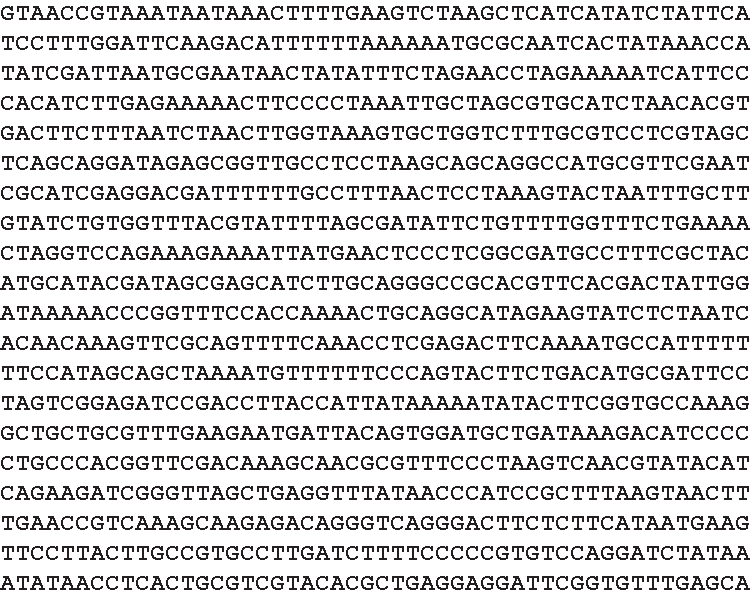
\includegraphics[width=10.8425in]{figs/genome-1kb-black}}
\center{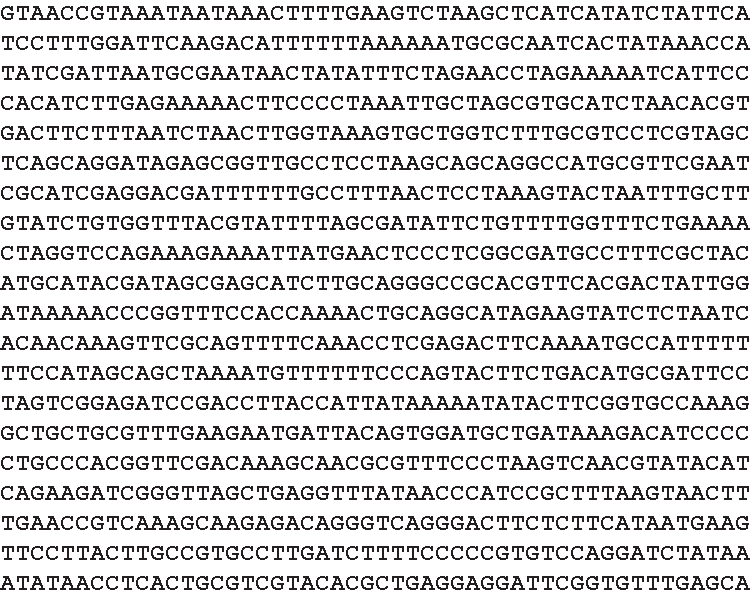
\includegraphics[height=8.34in]{figs/genome-1kb-black}}
\end{slide}
%%%%%%%%%%%%%%%%%%%%%%%%%%%%%%%%%%%%%%%%%%%%%%%%%%%%%%%%%%%%%%%%%%%%
\begin{slide}
\center{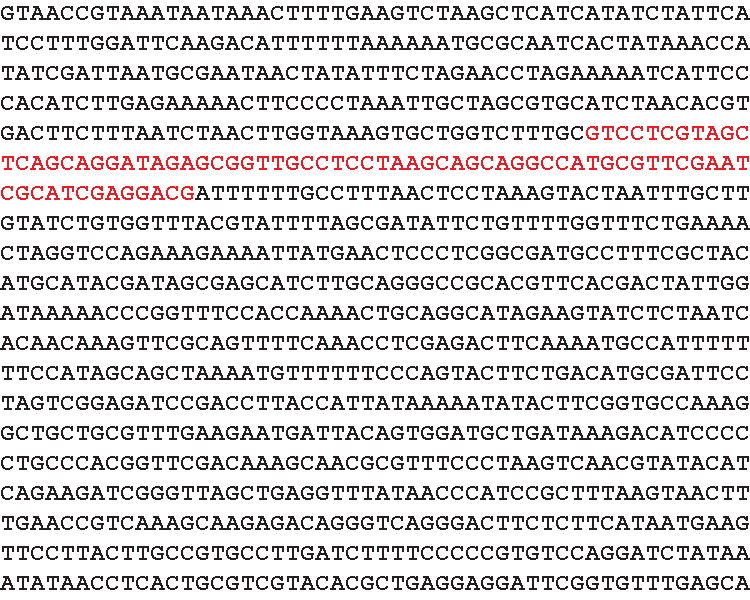
\includegraphics[height=8.34in]{figs/genome-1kb}}
\end{slide}
%%%%%%%%%%%%%%%%%%%%%%%%%%%%%%%%%%%%%%%%%%%%%%%%%%%%%%%%%%%%%%%%%%%%
\begin{slide}
\center{
\includegraphics[height=8.34in]{figs/genome-10kb}}
\end{slide}
%%%%%%%%%%%%%%%%%%%%%%%%%%%%%%%%%%%%%%%%%%%%%%%%%%%%%%%%%%%%%%%%%%%%
\begin{slide}
\center{
\includegraphics[height=8.34in]{figs/genome-100kb}}
\end{slide}
%%%%%%%%%%%%%%%%%%%%%%%%%%%%%%%%%%%%%%%%%%%%%%%%%%%%%%%%%%%%%%%%%%%%
\begin{comment}
\begin{slide}
\center{\includegraphics[height=8.34in]{figs/genome-full}}
\end{slide}
\end{comment}
%%%%%%%%%%%%%%%%%%%%%%%%%%%%%%%%%%%%%%%%%%%%%%%%%%%%%%%%%%%%%%%%%%%%
\begin{slide}
\begin{center}
\textbf{What are we looking for?}
\end{center}
\medskip

\begin{center}
\begin{tabular}{rl}
Protein-coding genes: & DNA $\rightarrow$ mRNA $\rightarrow$ protein \\
& \\
\textcolor{red}{Functional RNA genes:} & \textcolor{red}{DNA $\rightarrow$ RNA}
\end{tabular}
\medskip

\medskip

\medskip

\medskip

\medskip

\textbf{How can we find genes?}

\begin{tabular}{rl}
Gene family: & group of evolutionarily related ({\color{red}{\em homologous}}) \\
& genes in different genomes \\
& \\
Homology search: & given one or more homologs of a \\
& family, find more \\
\end{tabular}

%{\bf Functionally important sequence features are \\ evolutionarily conserved in
%  homologs.}

{\bf Homologous genes often share similar \\ functions, structures and
  sequences}

\end{center}

\vfill
\end{slide}
%%%%%%%%%%%%%%%%%%%%%%%%%%%%%%%%%%%%%%%%%%%%%%%%%%%%%%%%%%%%%%%
\begin{slide}
\begin{center}
{\bf Most proteins and RNAs adopt a conserved 3-dimensional 
  structure that is responsible for their function in the cell}

\medskip

Three representations of a transfer RNA:

%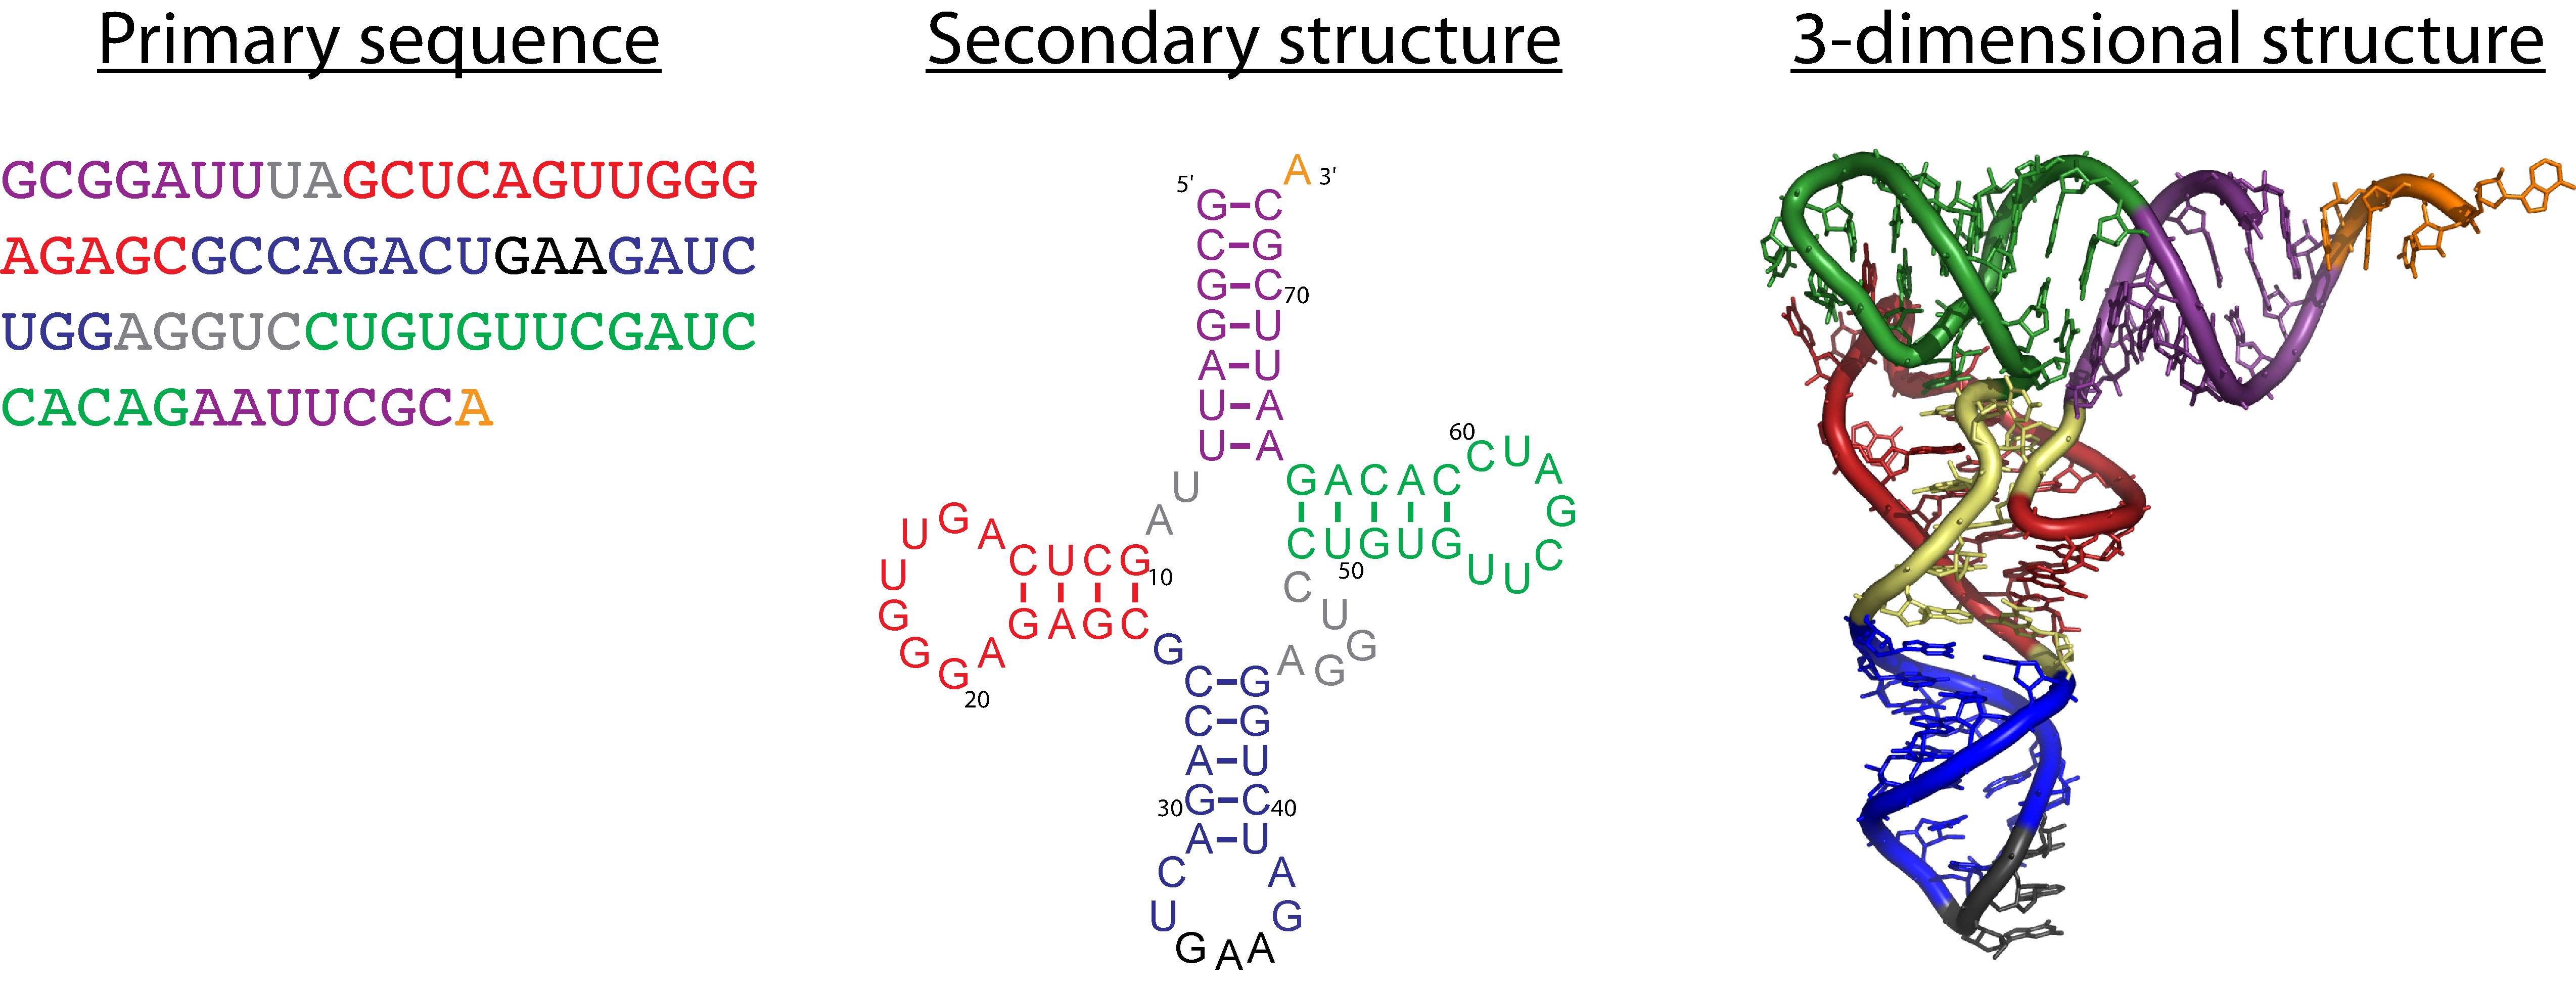
\includegraphics[width=10.5in]{figs/trna-123}
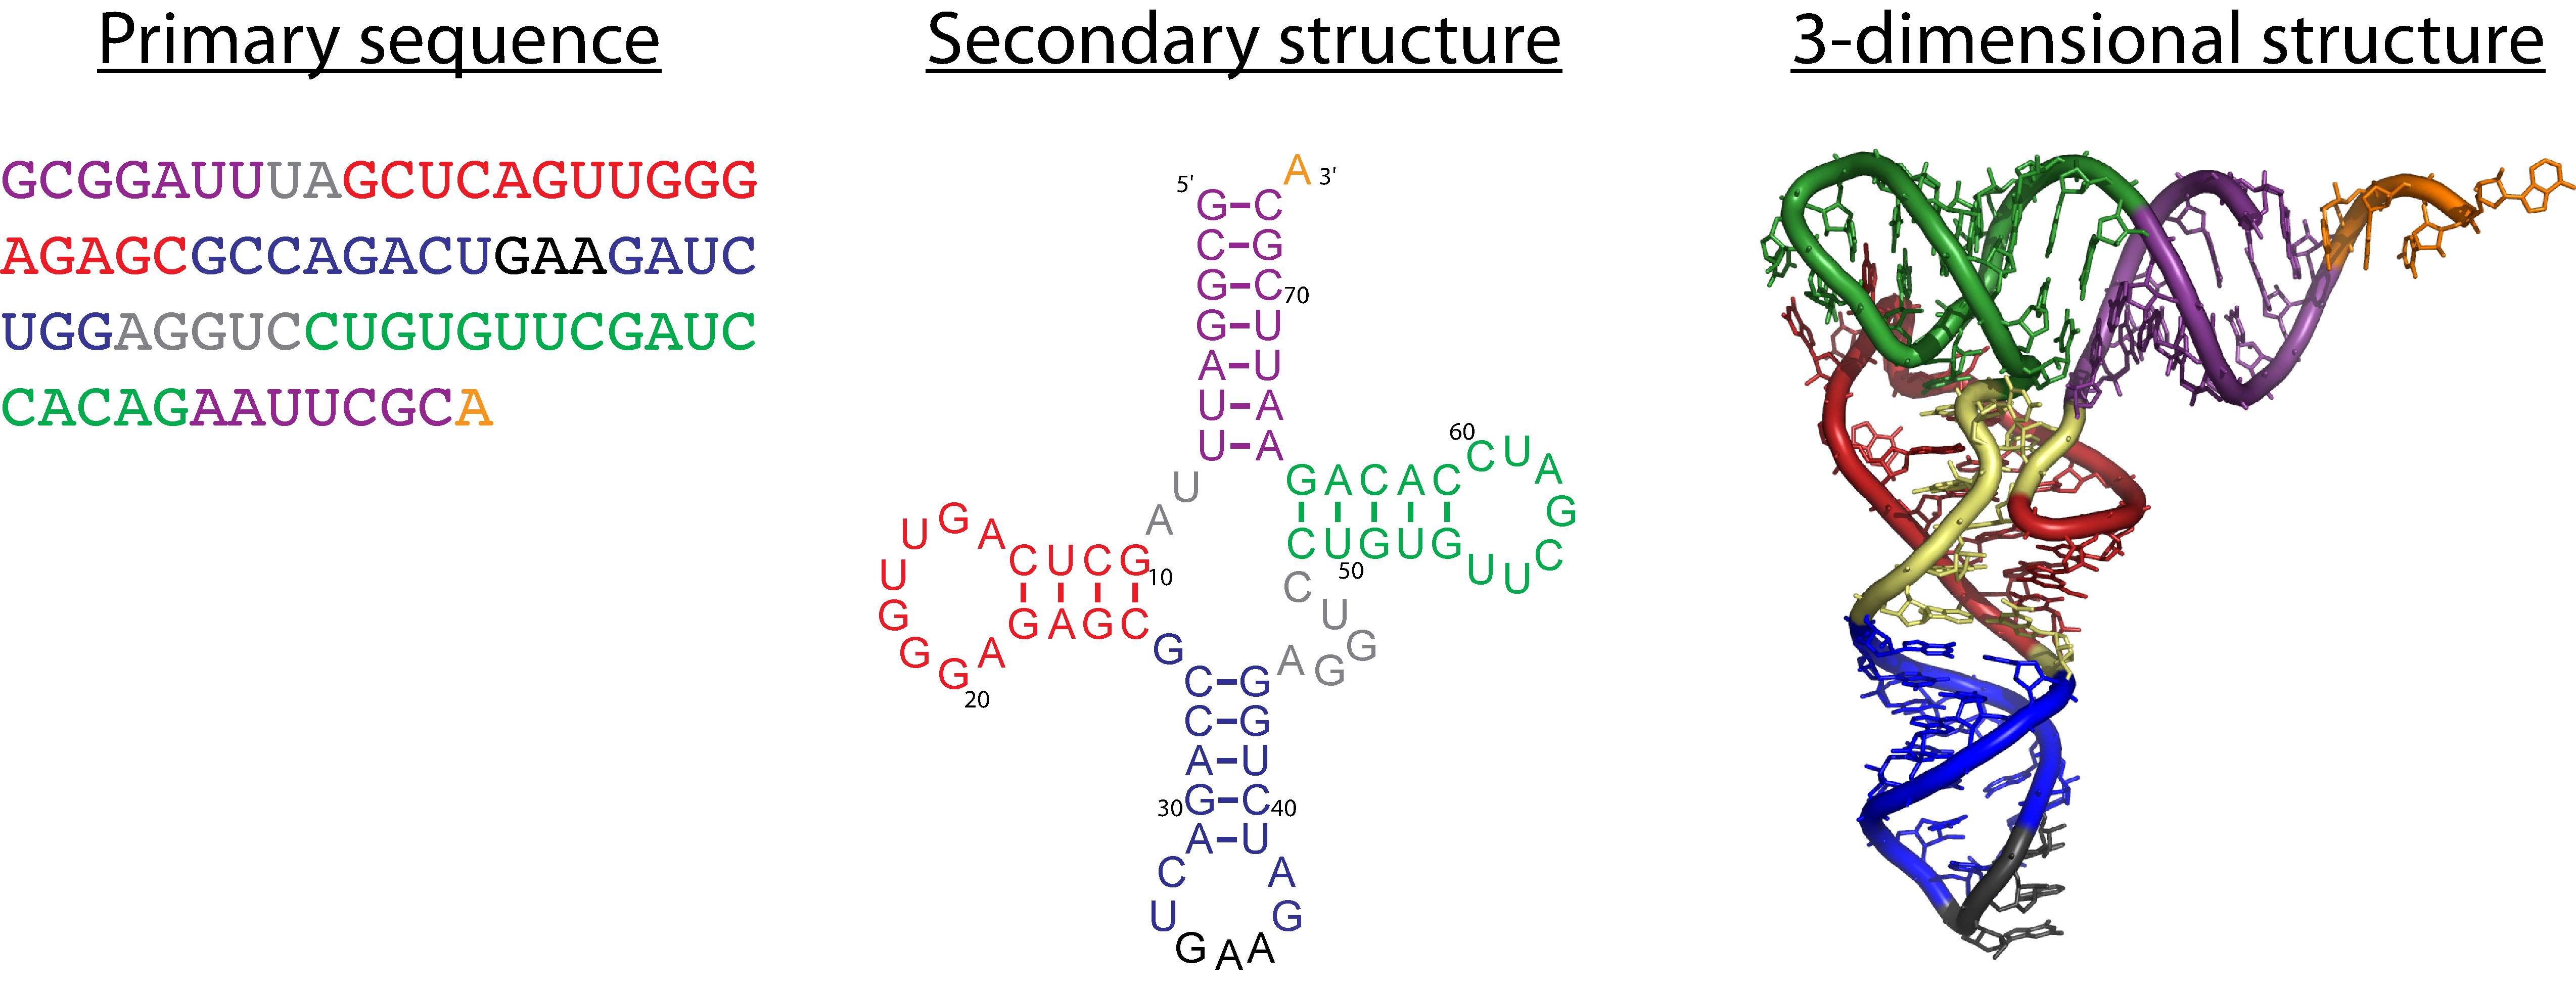
\includegraphics[width=9in]{figs/trna-123}

\end{center}

\vfill

\end{slide}
%%%%%%%%%%%%%%%%%%%%%%%%%%%%%%%%%%%%%%%%%%%%%%%%%%%%%%%%%%%%%%
\begin{slide}
\begin{center}
{\bf Most proteins and RNAs adopt a conserved 3-dimensional 
  structure that is responsible for their function in the cell}

\medskip

Three representations of a transfer RNA:

%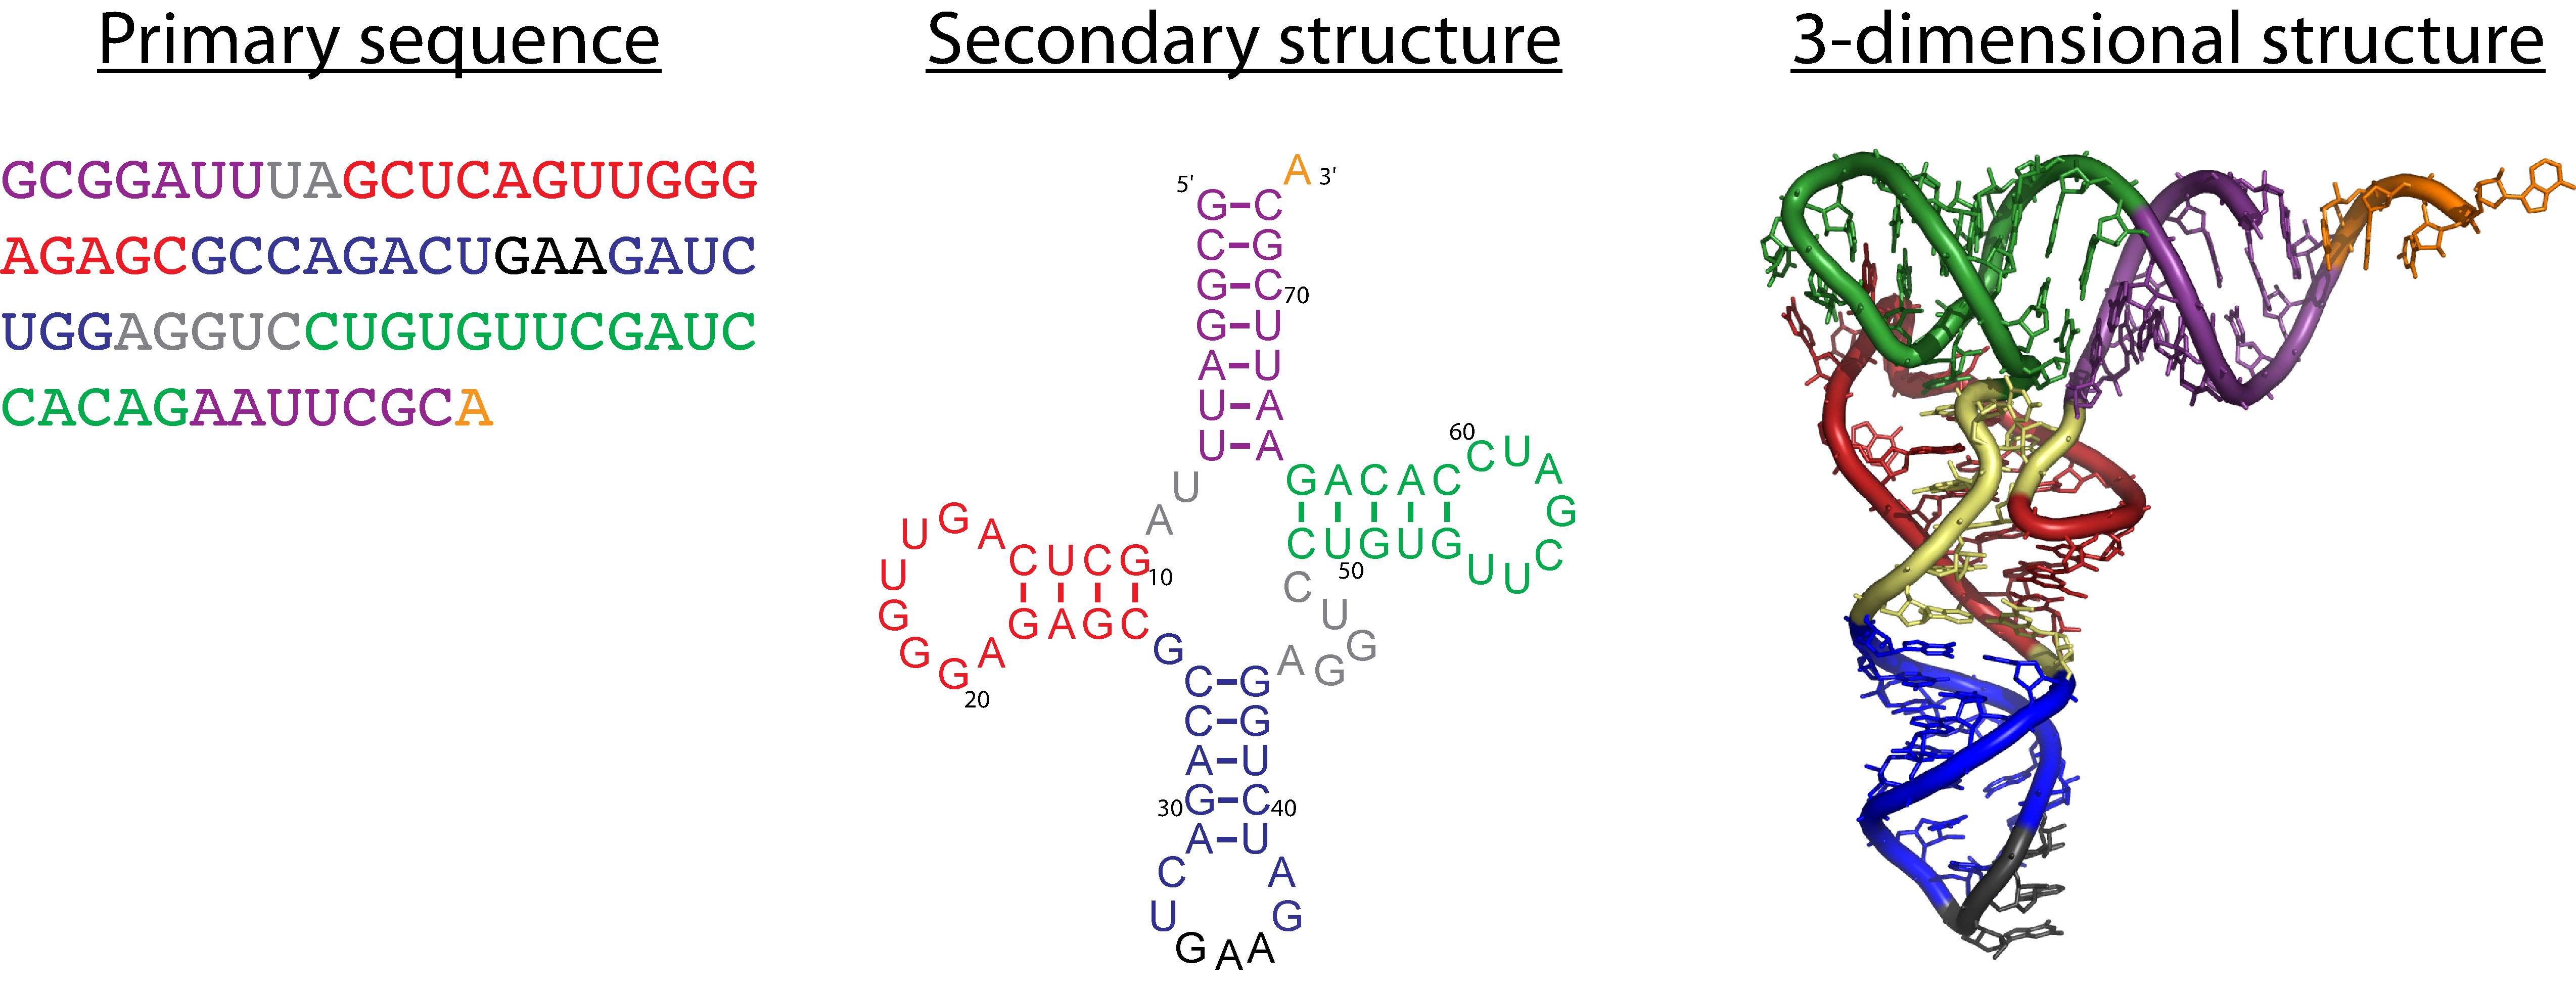
\includegraphics[width=10.5in]{figs/trna-123}
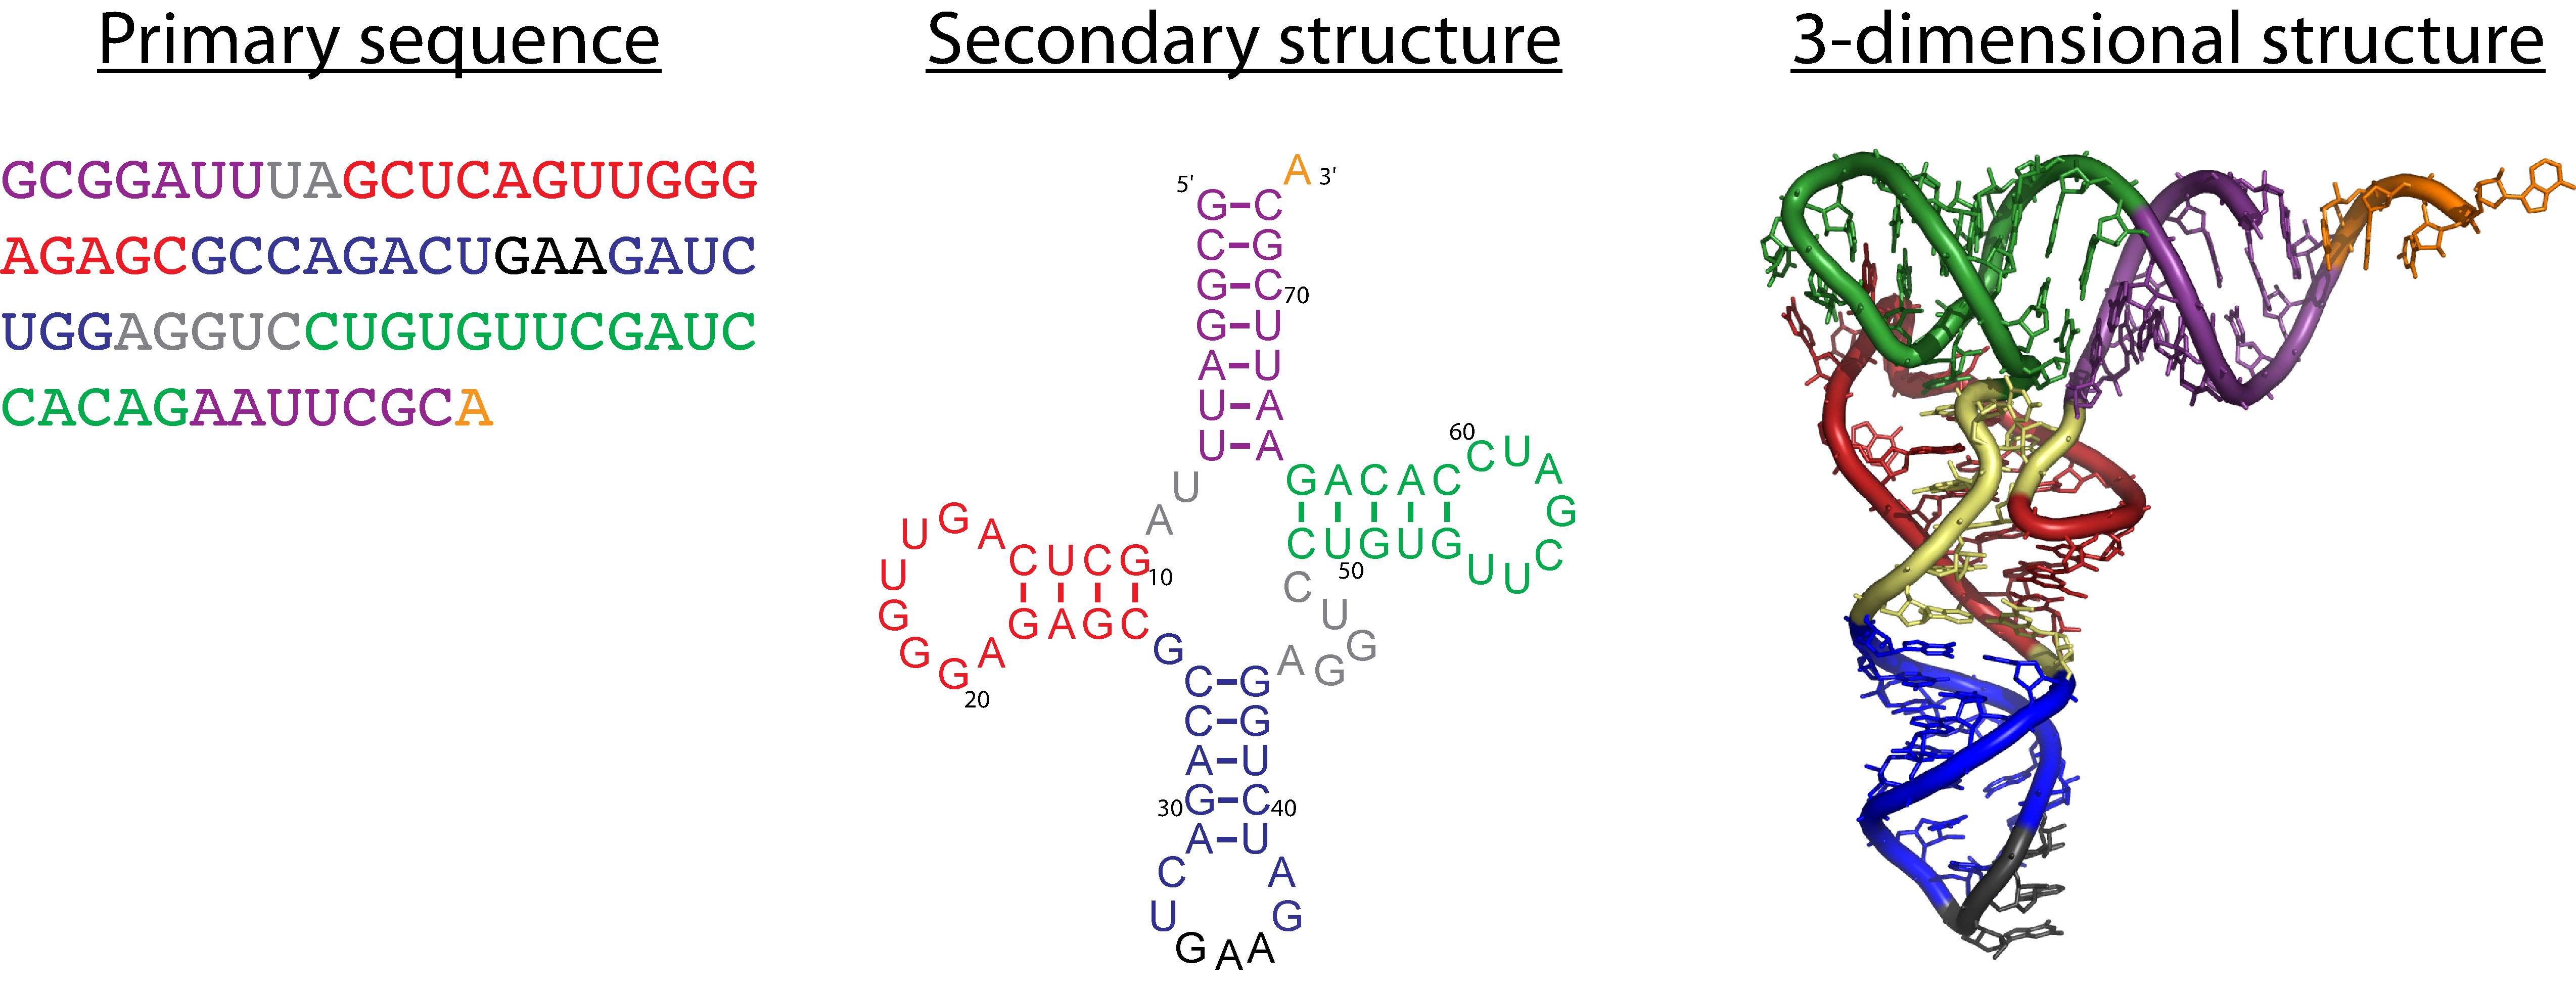
\includegraphics[width=9in]{figs/trna-123}

{\bf BLAST:} given a single sequence, search genomes for similar sequences.

%{\bf Homologous proteins and RNAs conserve \\ both sequence
%and structural features}

{\bf Homologous proteins and RNAs conserve different sequence \\
and structural features to different degrees.}
\end{center}

\vfill

\end{slide}
%%%%%%%%%%%%%%%%%%%%%%%%%%%%%%%%%%%%%%%%%%%%%%%%%%%%%%%%%%%%%
\begin{slide}
\begin{center}
%\textbf{Comparative analysis of sequence families}: \\
\textbf{Sequence conservation provides \\ information for homology searches}
%\emph{Functionally important sequence features are evolutionarily conserved.}
\medskip

%A simple, made-up RNA family:

%Evolution conserves functionally \\ important sequence features.

%Evolution conserves sequence \\ based on its functional importance.

Conservation levels vary across alignment columns.

%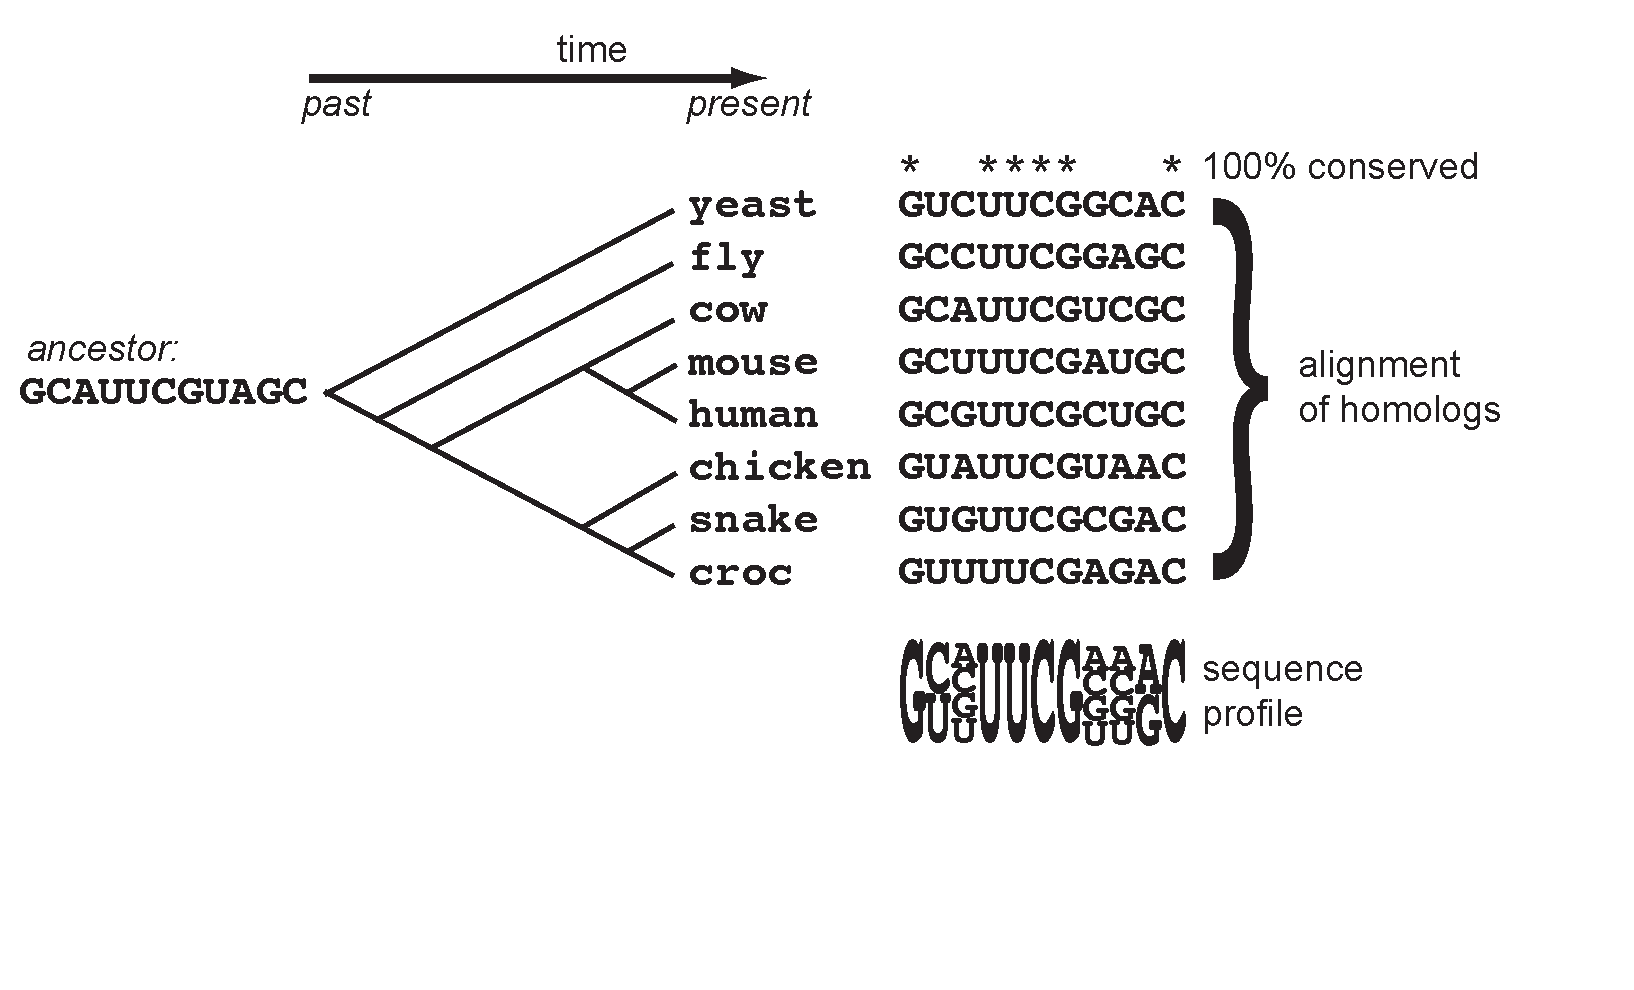
\includegraphics[width=9in]{figs/seqstructprofiles-seq1}
\includegraphics[width=9in]{figs/tmp}
\end{center}

\vfill
\end{slide}
%%%%%%%%%%%%%%%%%%%%%%%%%%%%%%%%%%%%%%%%%%%%%%%%%%%%%%%%%%%%%%%%%%%%%%
\begin{comment}
\begin{slide}
\begin{center}
\textbf{Structure conservation provides additional information}
\medskip

Base-paired positions covary \\ to maintain Watson-Crick complementarity.

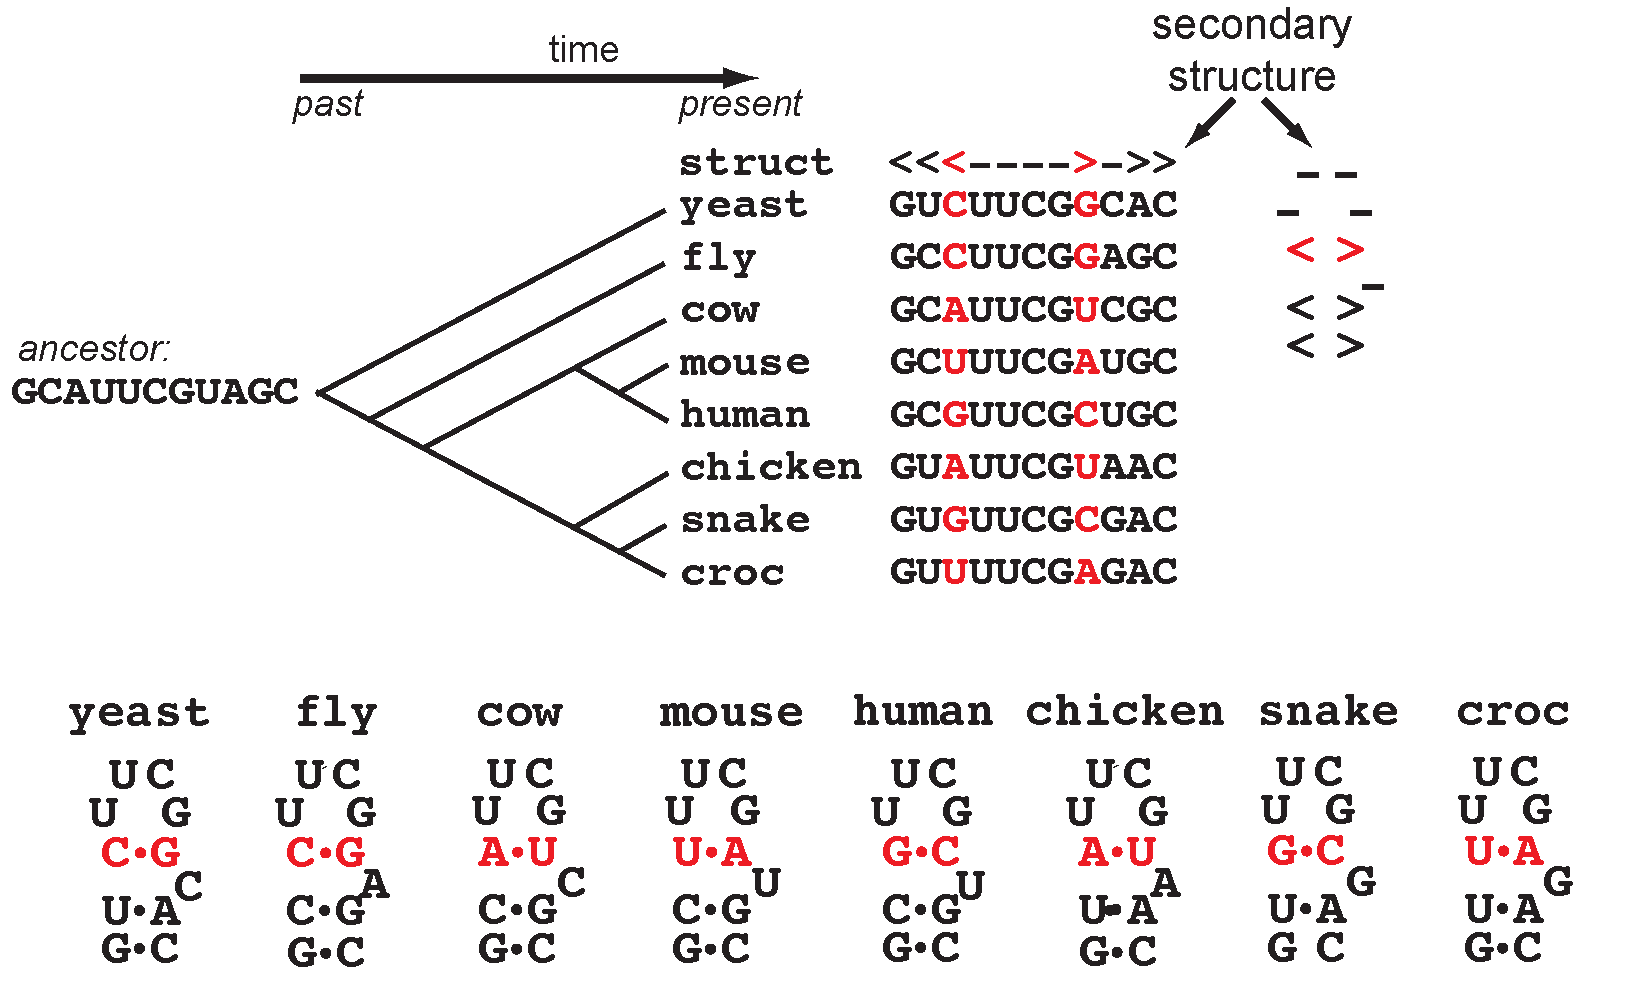
\includegraphics[width=9in]{figs/seqstructprofiles-struct1}
\end{center}

\vfill
\end{slide}
\end{comment}
%%%%%%%%%%%%%%%%%%%%%%%%%%%%%%%%%%%%%%%%%%%%%%%%%%%%%%%%%%%%%%%%%%%%%%
\begin{slide}
\begin{center}
\textbf{Structure conservation provides additional information}
\medskip

Base-paired positions covary \\ to maintain Watson-Crick complementarity.

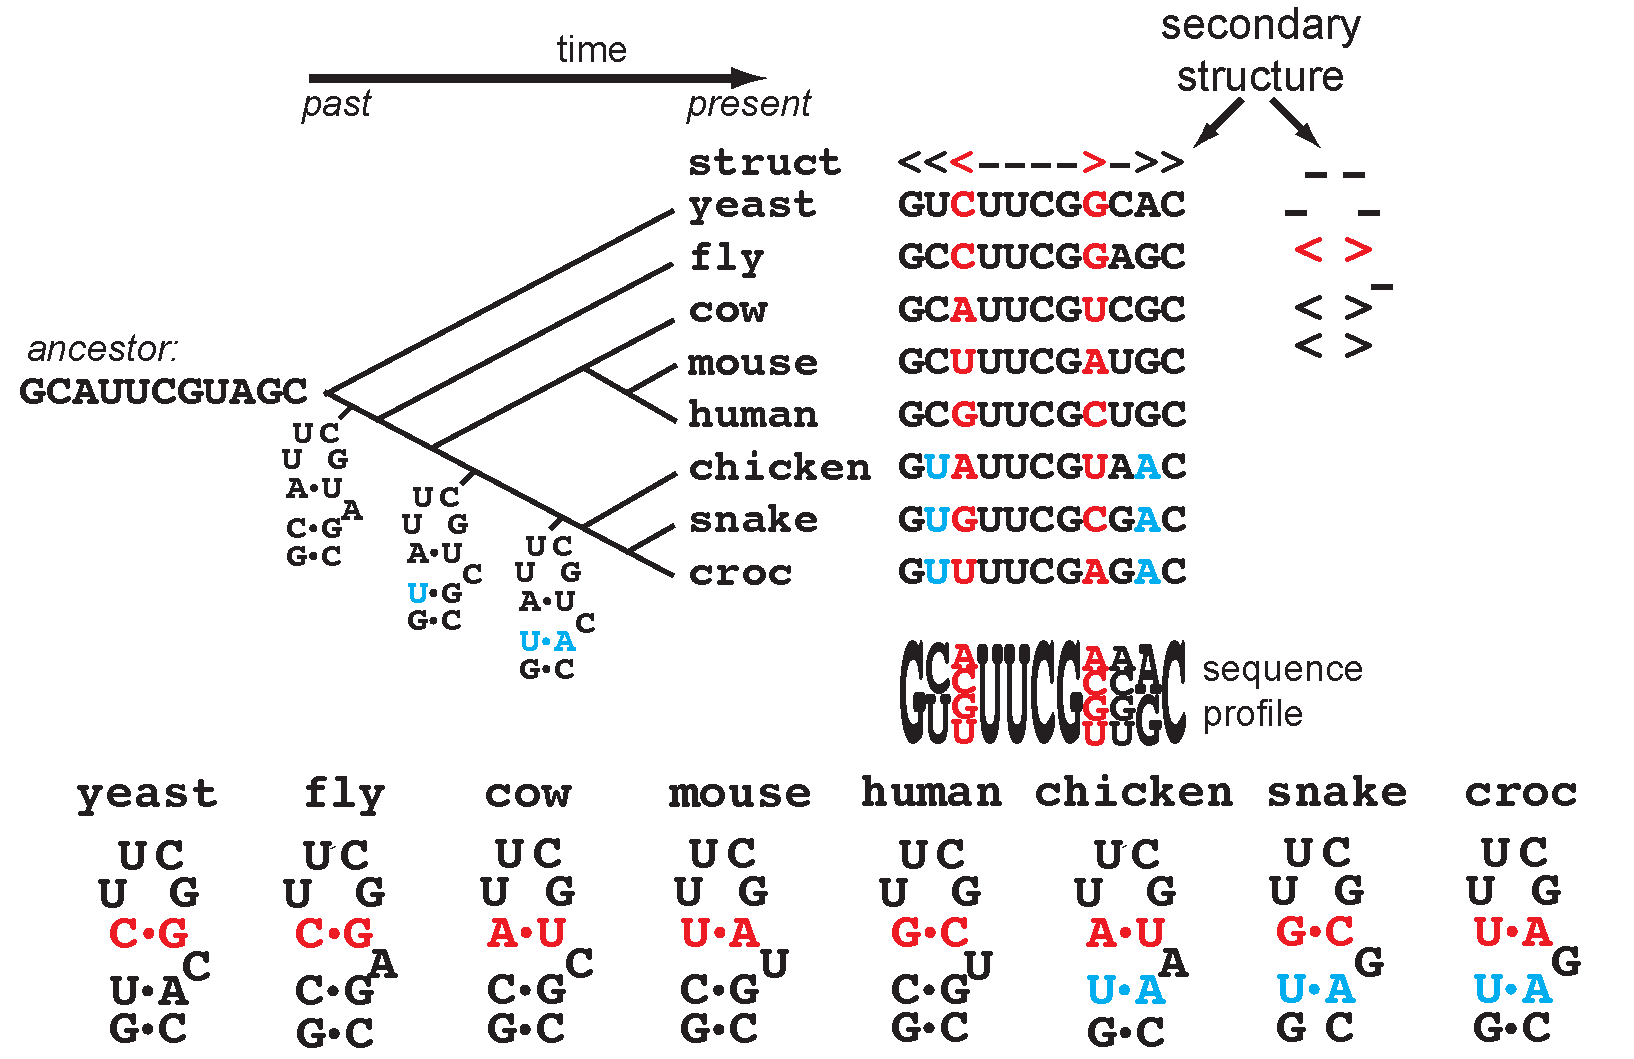
\includegraphics[width=9in]{figs/seqstructprofiles-struct2}
\end{center}

\vfill
\end{slide}
%%%%%%%%%%%%%%%%%%%%%%%%%%%%%%%%%%%%%%%%%%%%%%%%%%%%%%%%%%%%%%%%%%%%%%%%%%
\begin{slide}
\begin{center}
\textbf{Levels of sequence and structure conservation in RNA families}
\end{center}
\medskip

\begin{center}
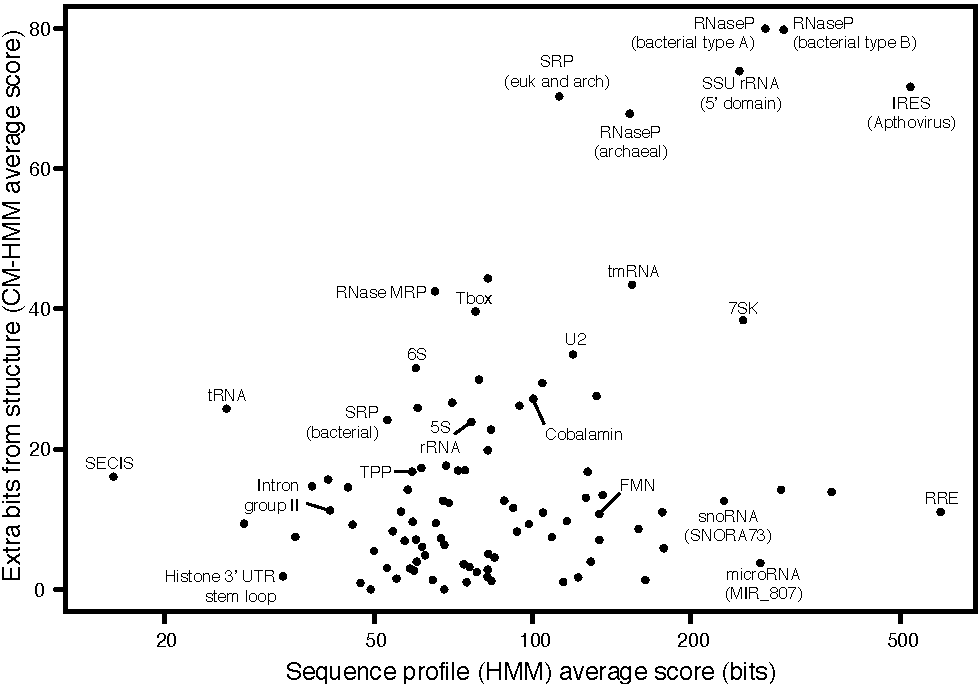
\includegraphics[height=6.5in]{figs/avgscores}
\end{center}

\vfill

\end{slide}
%%%%%%%%%%%%%%%%%%%%%%%%%%%%%%%%%%%%%%%%%%%%%%%%%%%%%%%%%%%%%%%%%%%
\begin{slide}
\begin{center}
%\textbf{profile HMMs and covariance models}
\textbf{Eddy lab software for profile probabilistic models} \\
(since 1994)
\end{center}
\medskip

\begin{center}
\small
\begin{tabular}{r|cc} 
%             &         & sequence \\
%             & sequence& and structure \\
%             & profiles& profiles \\ \hline
             & sequence & sequence and \\
             & profiles & structure profiles \\ \hline
  \\
  models     & profile HMMs    & {\color{red} covariance models (CMs)} \\ 
  \\
  software   & {\sc HMMER}     & {\sc Infernal} \\ 
             &                 & (prev. COVE) \\
  \\
  main use   & proteins        & RNAs \\ 
  \\
  database   & {\sc Pfam}      & {\sc Rfam} \\
             & (9318 families) & (1371 families) \\
  \\
%  primary sequence & yes & yes \\
%  \\
%  secondary structure & no & yes \\
%  \\
%  algorithms & Viterbi, Forward & CYK, Inside \\
%%             & Forward & Inside \\
%             &         & \\
%  complexity & $O(LN)$ & $O(LN^{2} log N)$ \\
%  \\
  performance& faster but    & slower but    \\
  for RNAs   & less accurate & more accurate \\
\end{tabular}

%\hspace{1.2in}
\includegraphics[height=2in]{figs/hmmer_logo}\hspace{1.05in}
\includegraphics[height=2.6in]{figs/infernal_logo}
\hspace{1.2in}
\includegraphics[height=2.7in]{figs/hmmer-infernal-refs}

\end{center}

\vfill

\end{slide}
%%%%%%%%%%%%%%%%%%%%%%%%%%%%%%%%%%%%%%%%%%%%%%%%%%%%%%%%%%%%%%%
%%%%%%%%%%%%%%%%%%%%%%%%%%%%%%%%%%%%%%%%%%%%%%%%%%%%%%%%%%%%%%%%%%%%
\begin{slide}
\begin{center}
%\textbf{profile HMMs and covariance models}
\textbf{Profile HMMs: sequence family models built from alignments}
\end{center}
\medskip

\center{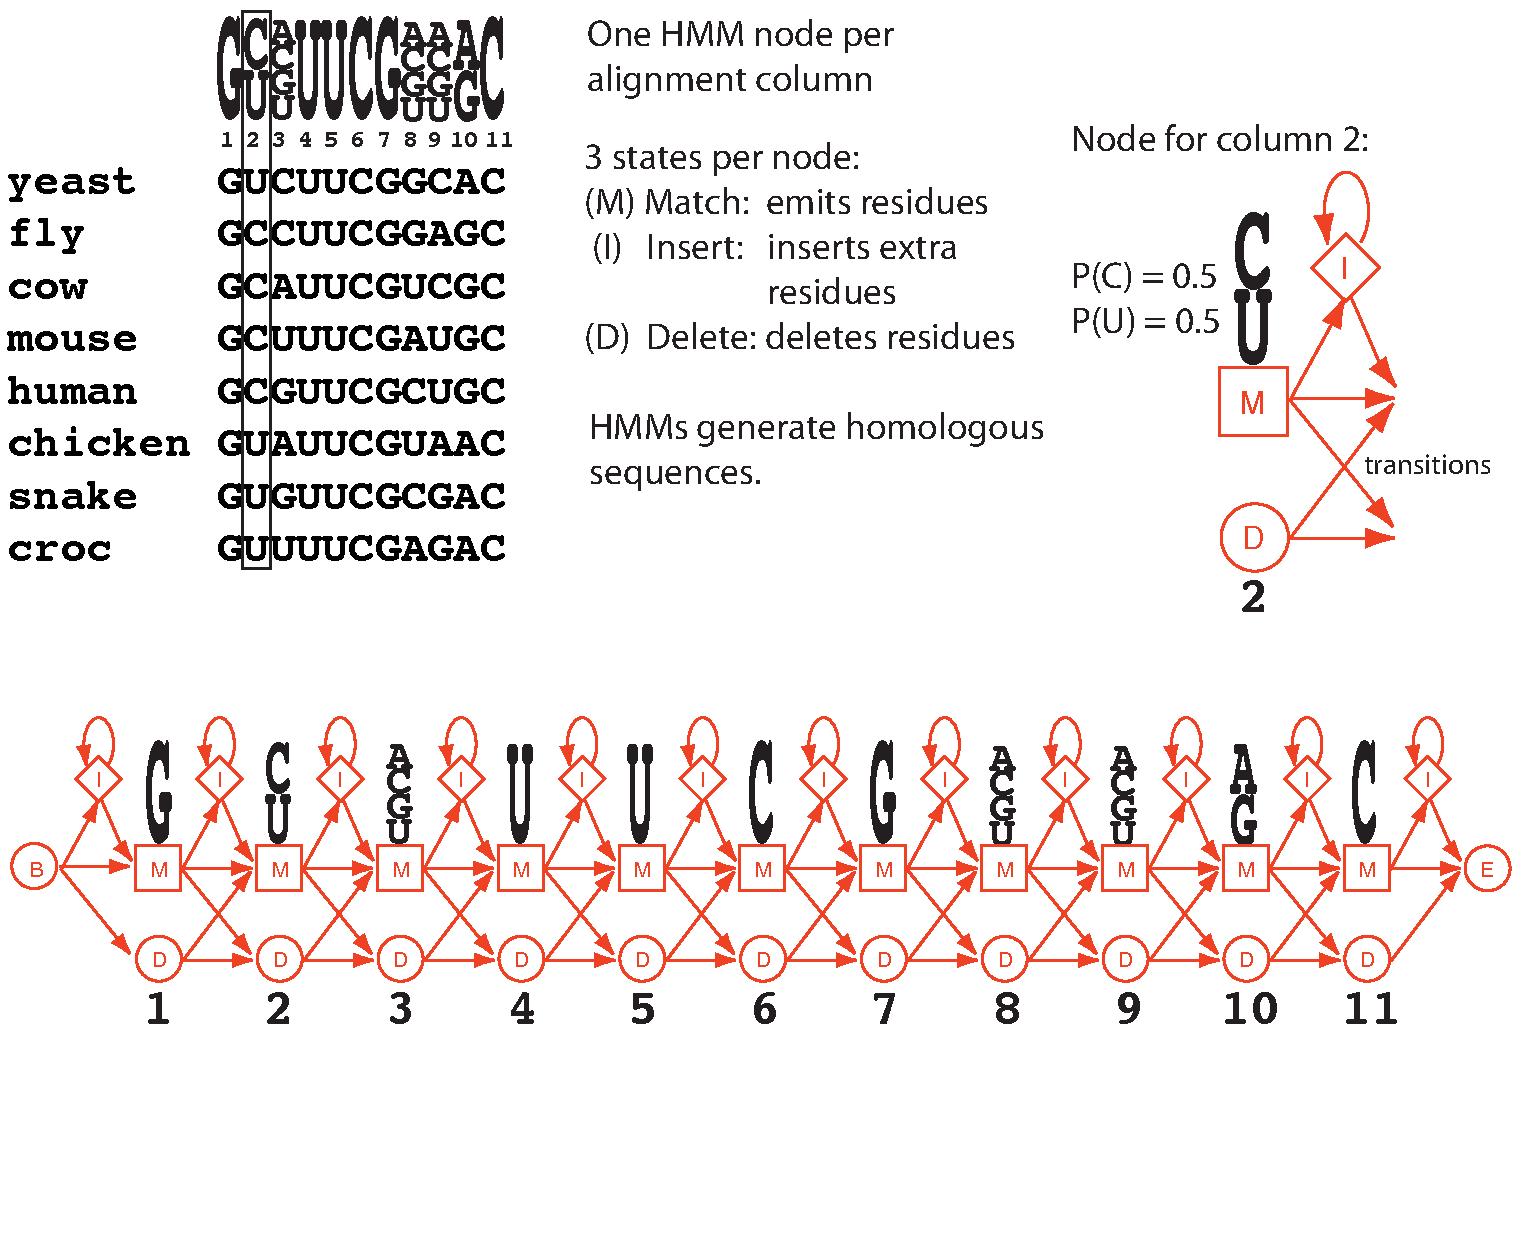
\includegraphics[height=7in]{figs/hmm}}

%An HMM generates ``homologous'' sequences.

\end{slide}
%%%%%%%%%%%%%%%%%%%%%%%%%%%%%%%%%%%%%%%%%%%%%%%%%%%%%%%%%%%%%%%
\begin{slide}
\begin{center}
%\textbf{profile HMMs and covariance models}
\textbf{Profile HMMs: sequence family models built from alignments}
\end{center}
\medskip

\center{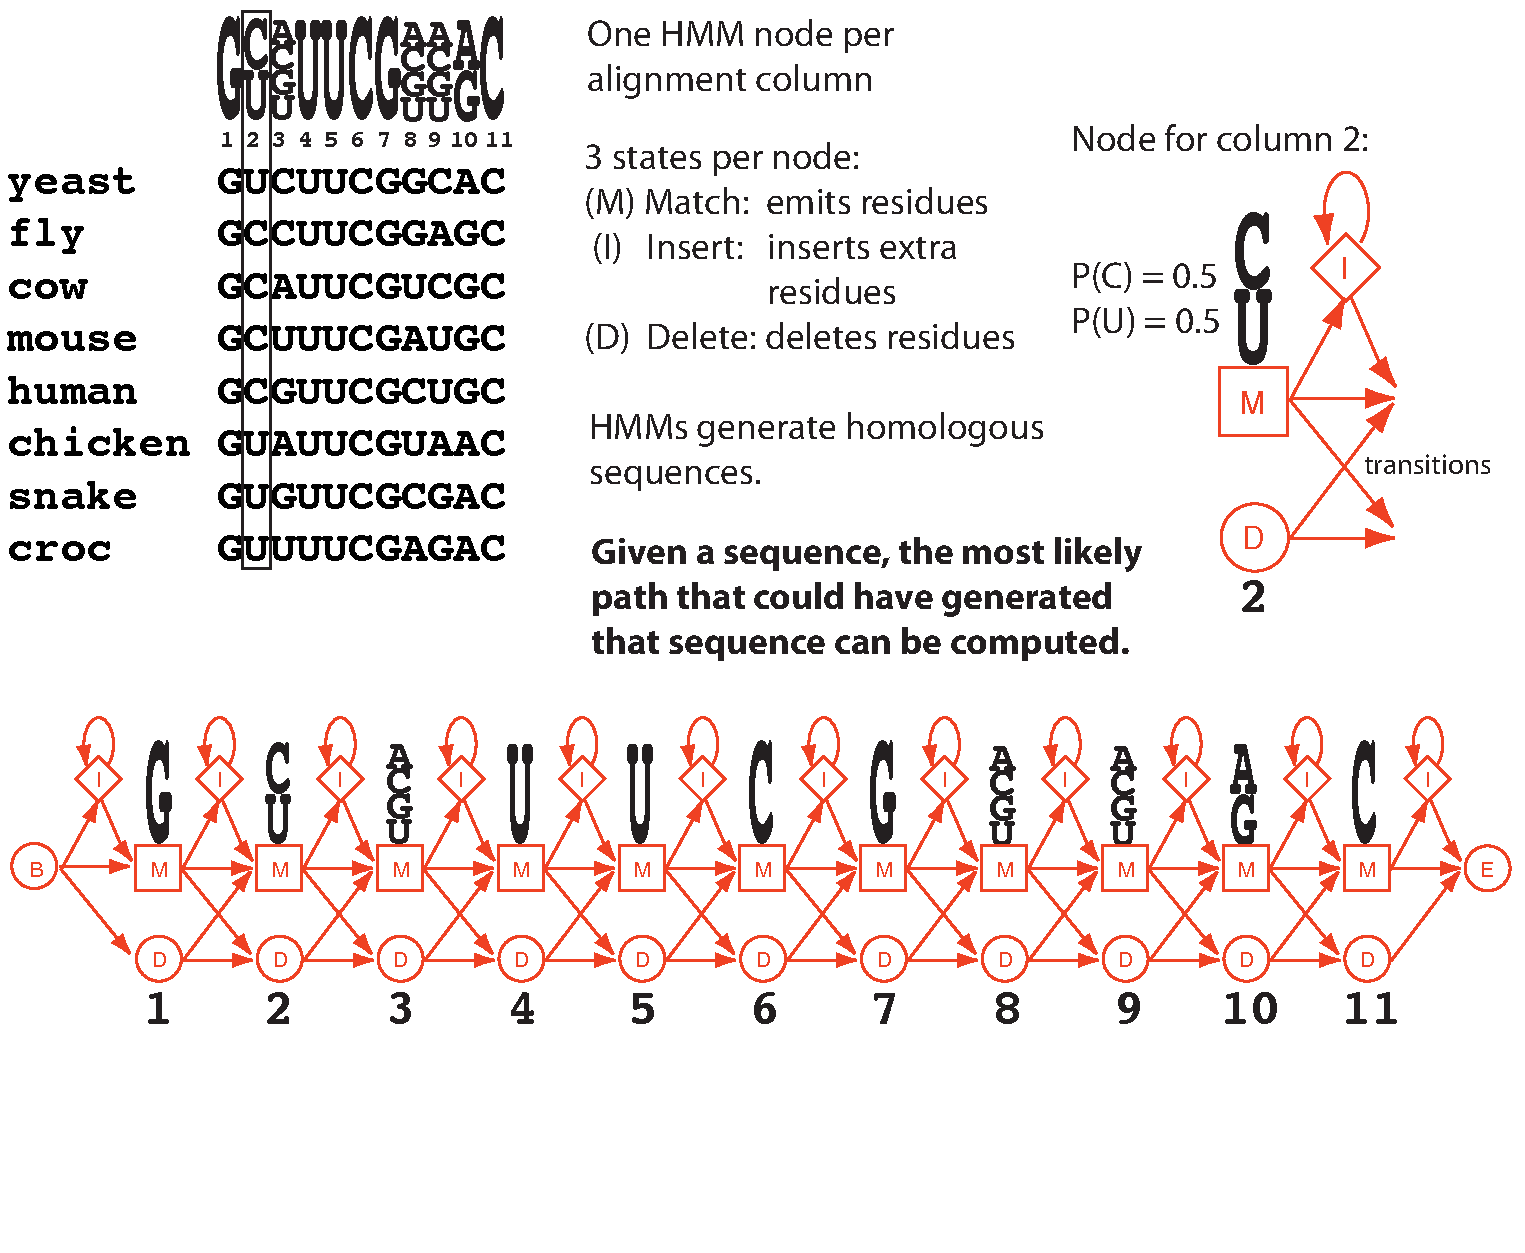
\includegraphics[height=7in]{figs/hmm-given}}
\end{slide}
%%%%%%%%%%%%%%%%%%%%%%%%%%%%%%%%%%%%%%%%%%%%%%%%%%%%%%%%%%%%%%%
\begin{slide}
\begin{center}
%\textbf{profile HMMs and covariance models}
\textbf{Profile HMMs: sequence family models built from alignments}
\end{center}
\medskip

\center{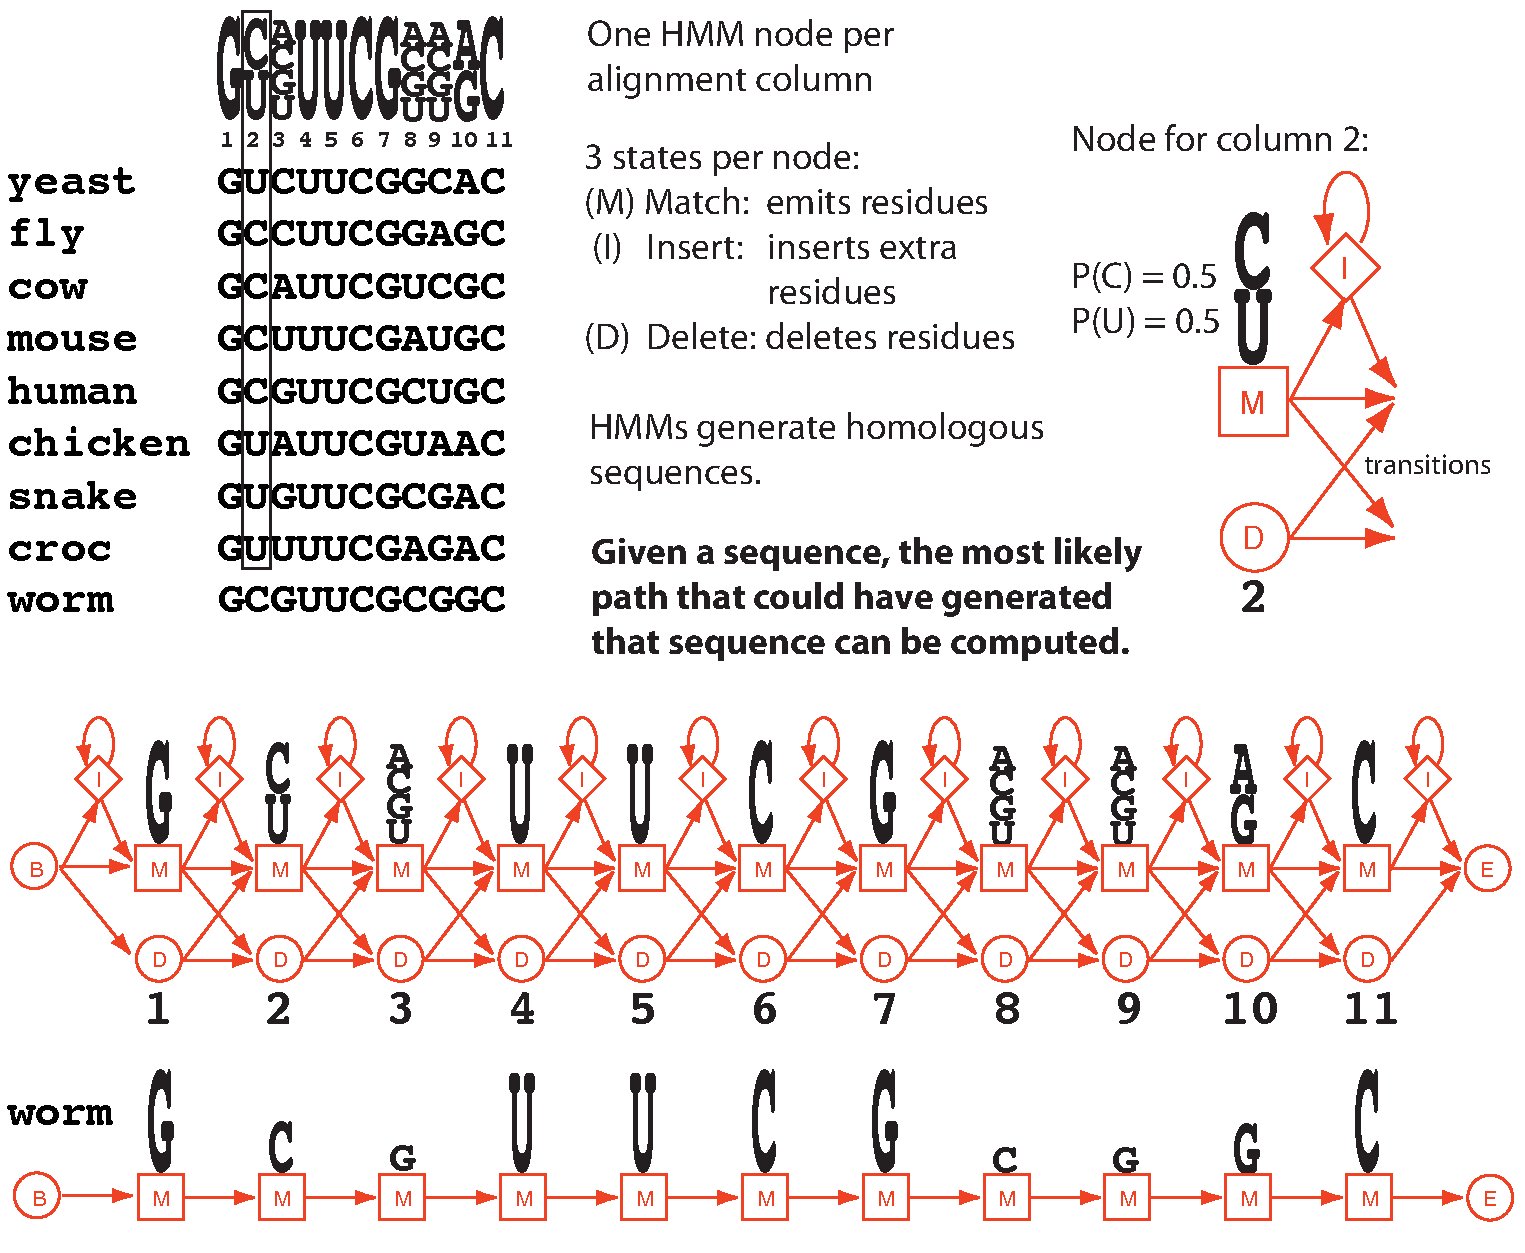
\includegraphics[height=7in]{figs/hmm-worm}}
\end{slide}
%%%%%%%%%%%%%%%%%%%%%%%%%%%%%%%%%%%%%%%%%%%%%%%%%%%%%%%%%%%
\begin{slide}
\begin{center}
%\textbf{profile HMMs and covariance models}
\textbf{Profile HMMs: sequence family models built from alignments}
\end{center}
\medskip

\center{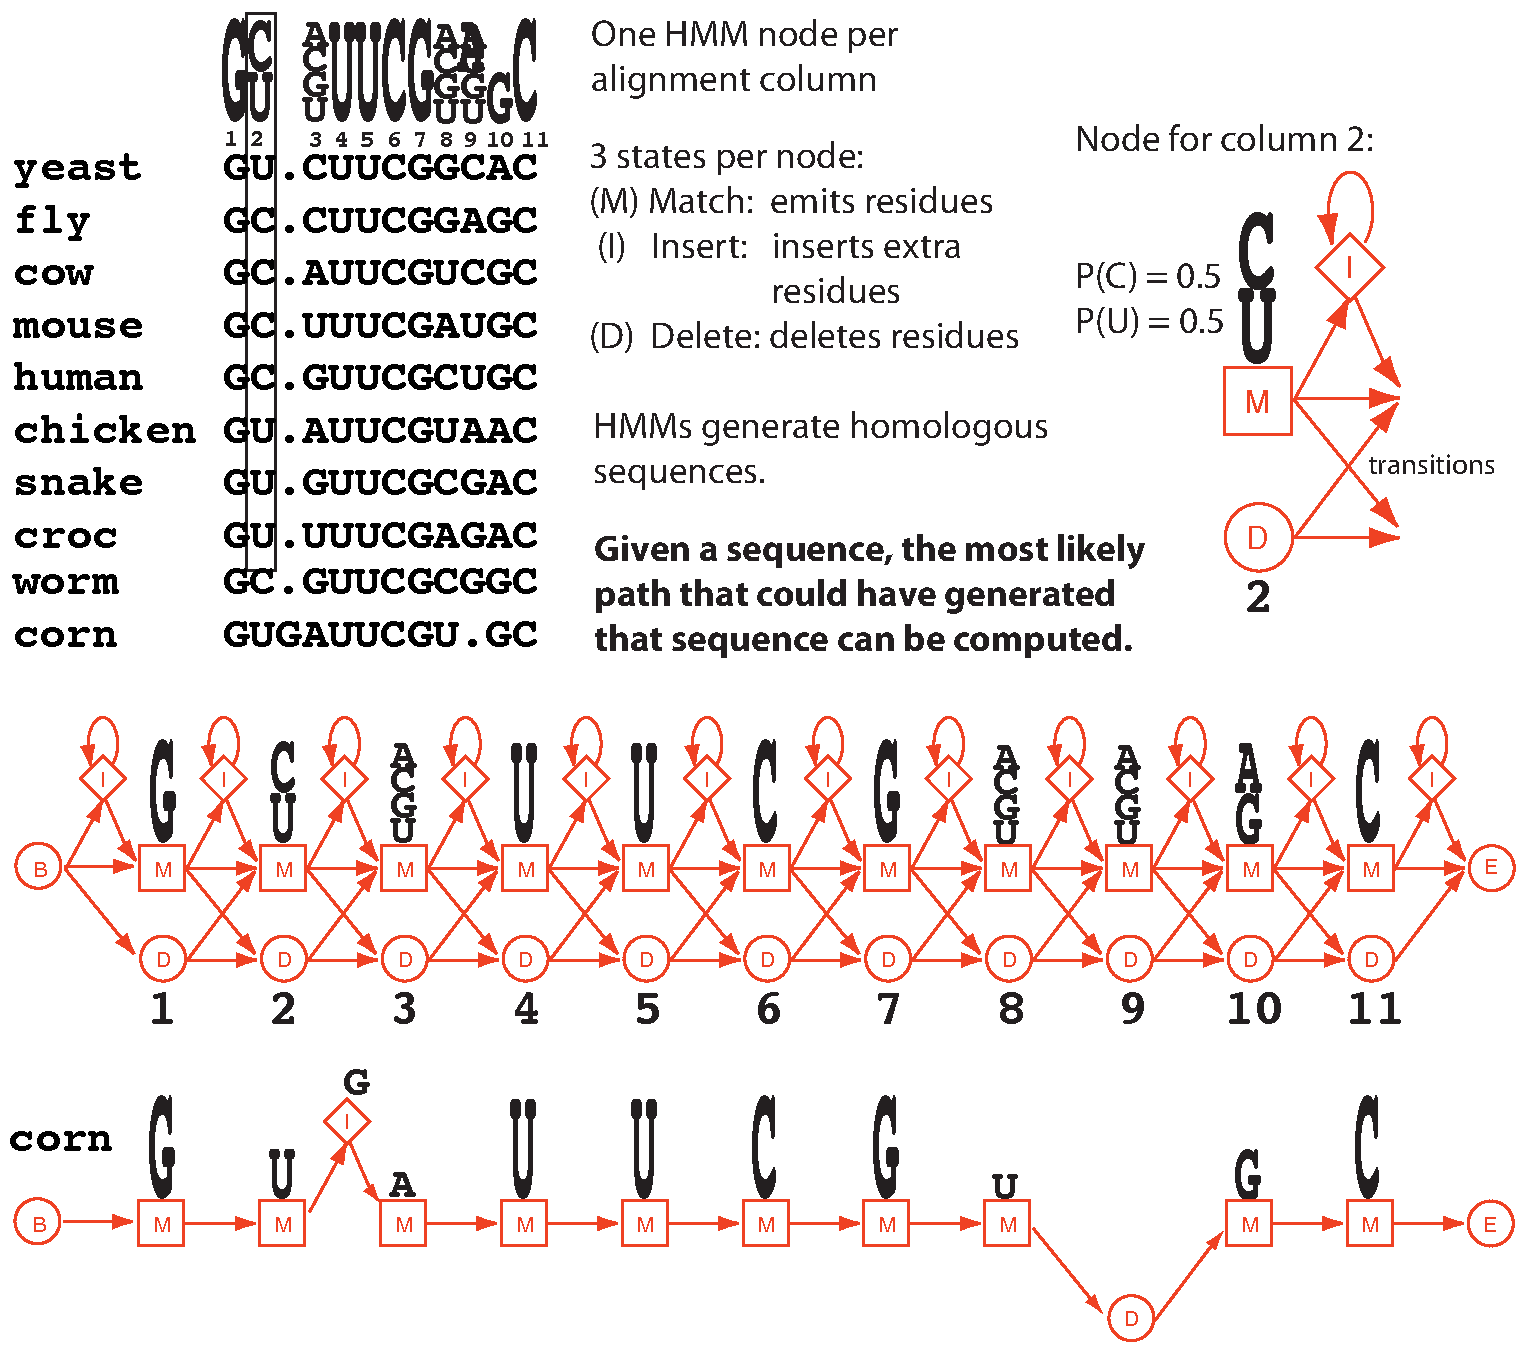
\includegraphics[height=7in]{figs/hmm-corn}}
\end{slide}
%%%%%%%%%%%%%%%%%%%%%%%%%%%%%%%%%%%%%%%%%%%%%%%%%%%%%%%%%%%%%%%
\begin{slide}
\begin{center}
%\textbf{profile HMMs and covariance models}
\textbf{Covariance models (CMs) are built \\ from structure-annotated alignments}
\end{center}
\medskip

\center{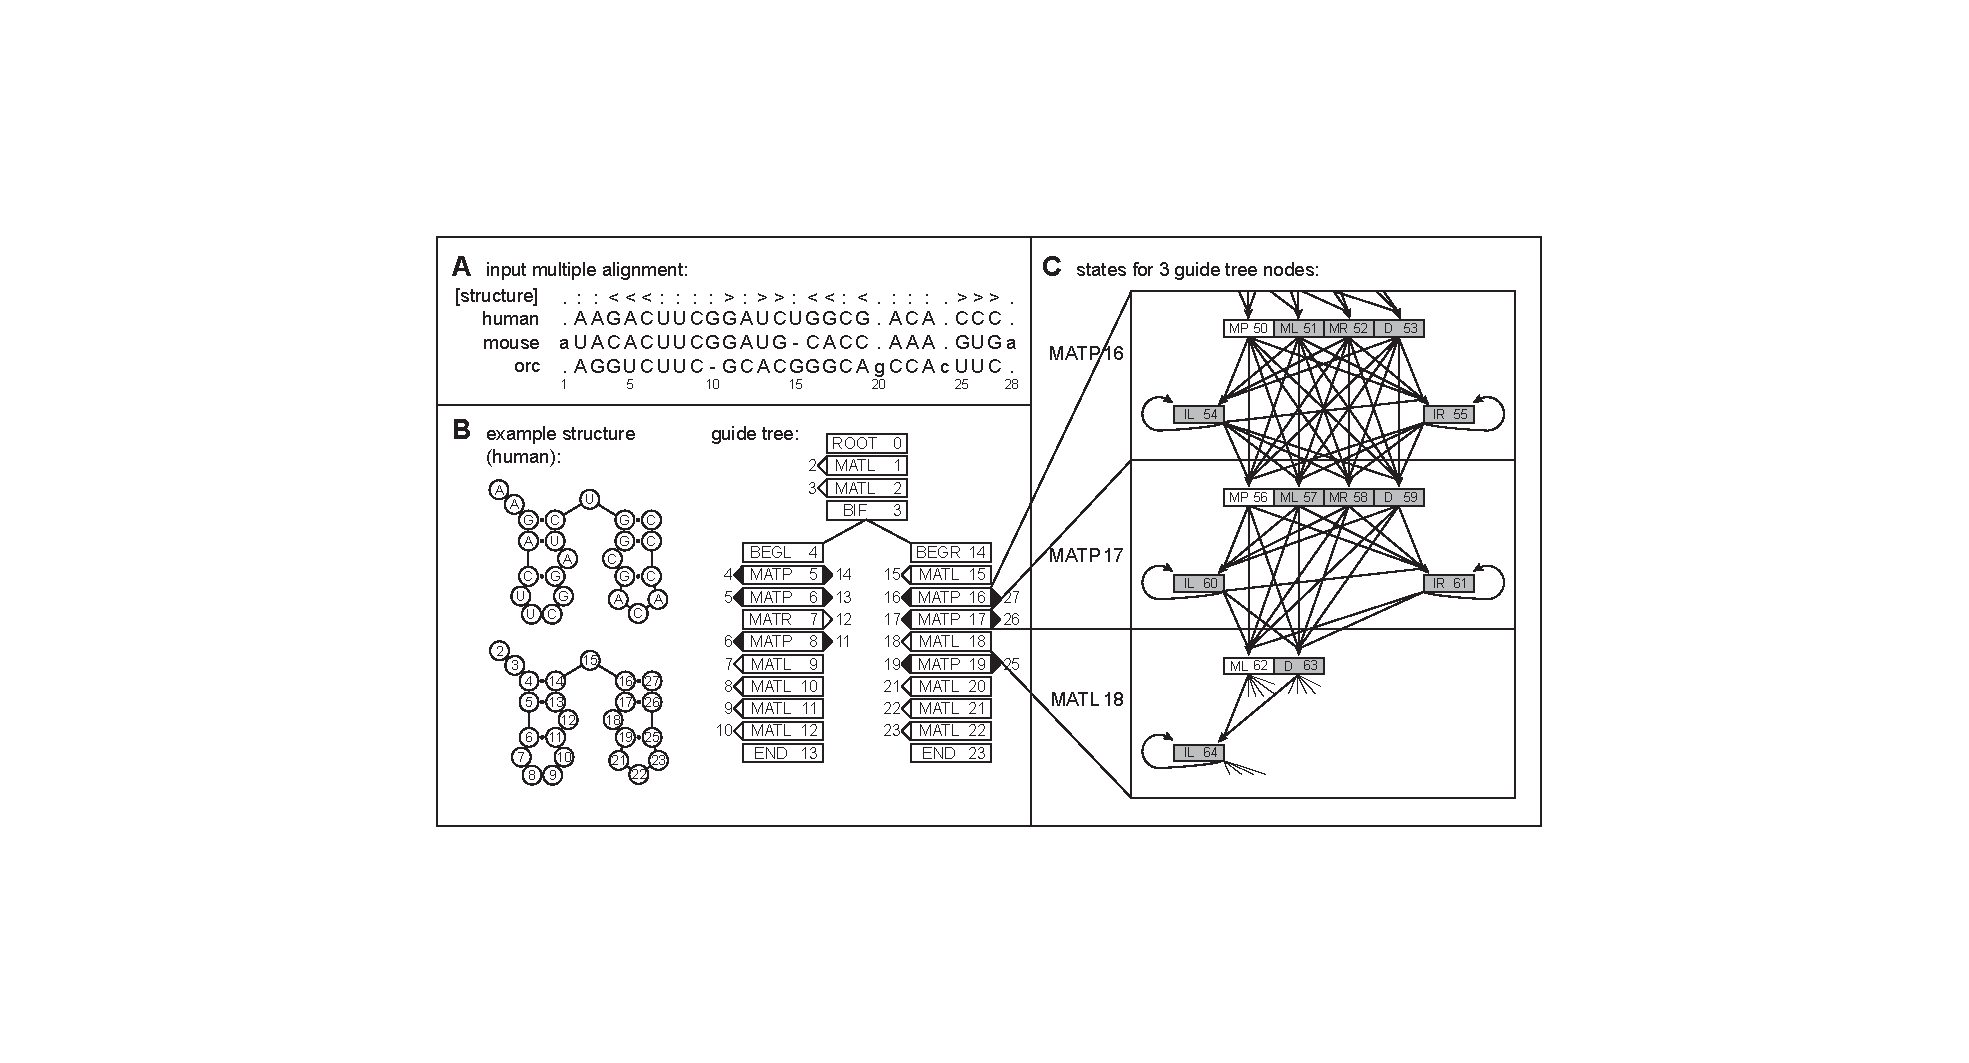
\includegraphics[width=8in]{figs/cmintro_bandcyk}}

\center{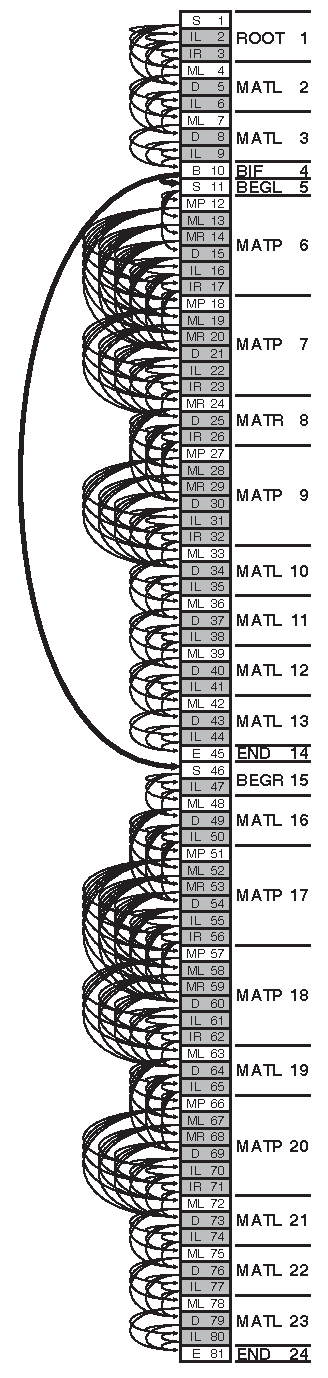
\includegraphics[width=2in,angle=270]{figs/cm-graph-small}}

%\item Extensions of profile HMMs that 

%\item Generative models that generate ``homologous'' structural RNA sequences

\vfill

\end{slide}
%%%%%%%%%%%%%%%%%%%%%%%%%%%%%%%%%%%%%%%%%%%%%%%%%%%%%%%%%%%%%%%%%%%%
\begin{slide}
\begin{center}

\textbf{My work on Infernal}
\medskip

\small 
\begin{itemize}
\item Infernal version 0.55 existed when I entered the lab.

\item I have developed and implemented methods for:

\begin{itemize}
\item improving the accuracy of CM searches 
\item accelerating CM searches 
\item accelerating CM alignment 
\end{itemize}
\end{itemize}

\begin{tabular}{l}
Nawrocki EP. Eddy SR. PLoS Comput. Biol., 3:e56, 2007. \\
\\
Nawrocki EP. Kolbe DL. Eddy SR. Bioinformatics, 25:1335-1337, 2009. \\
\end{tabular}
\end{center}

\vfill 
\end{slide}
%%%%%%%%%%%%%%%%%%%%%%%%%%%%%%%%%%%%%%%%%%%%%%%%%%%%%%%%%%%%%%%%%%%%
\begin{slide}
\begin{center}

\textbf{My work on Infernal}
\medskip

\small 
\begin{itemize}
\item Infernal version 0.55 existed when I entered the lab.

\item I have developed and implemented methods for:

\begin{itemize}
\item improving the accuracy of CM searches
\item accelerating CM searches
\item accelerating CM alignment
\end{itemize}
\end{itemize}

\begin{tabular}{l}
Nawrocki EP, Eddy SR. PLoS Comput. Biol., 3:e56, 2007. \\
\\
Nawrocki EP, Kolbe DL, Eddy SR. Bioinformatics, 25:1335-1337, 2009. \\
\end{tabular}
\end{center}

\bigskip

\small 
\begin{itemize}
\item First, I constructed a benchmark to evaluate homology search performance.

\item Performance is judged by:
  \begin{itemize}
    \item sensitivity: correctly inferring homology 
    \item specificity: correctly ignoring non-homology 
  \end{itemize}
\end{itemize}

\vfill 
\end{slide}
%%%%%%%%%%%%%%%%%%%%%%%%%%%%%%%%%%%%%%%%%%%%%%%%%%%%%%%%%%%%%%%%%%%%%%%%%%
\begin{slide}
\begin{center}

\textbf{Infernal v0.55 does no better than sequence-only profiles (HMMs)}
\end{center}
\medskip

\center{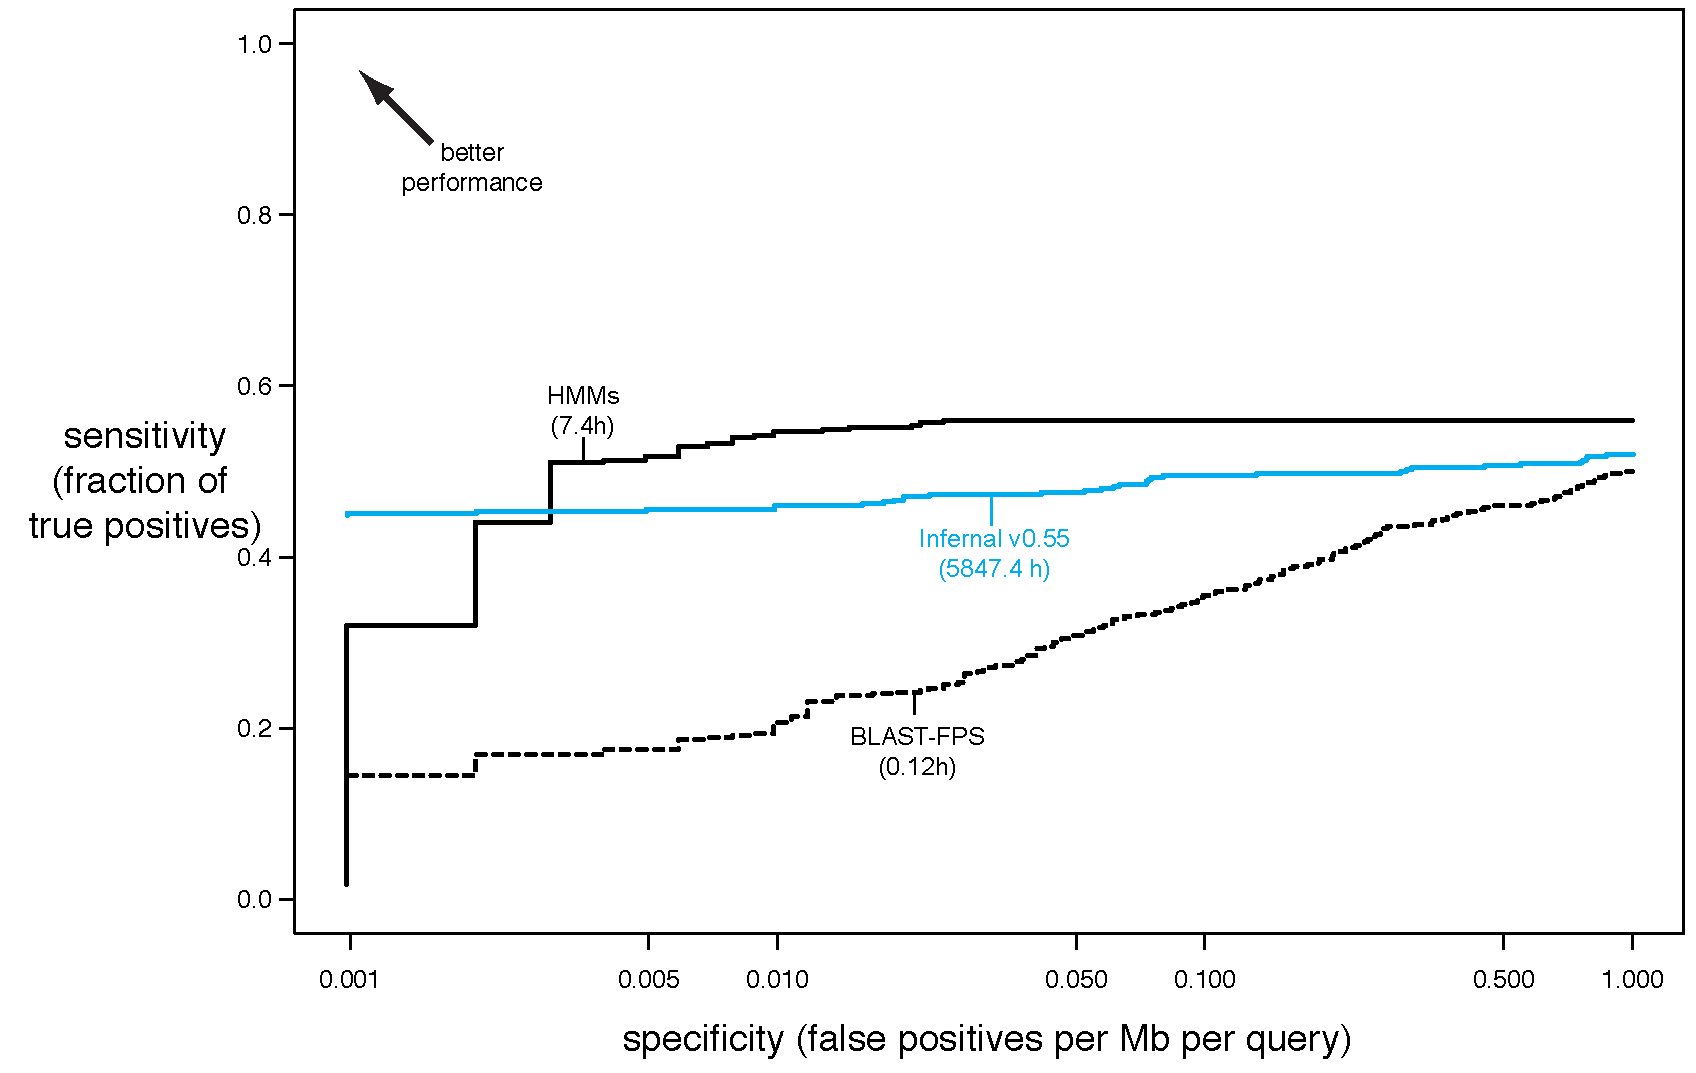
\includegraphics[width=10in]{figs/defense-roc1}}

\vfill 
\end{slide}
%%%%%%%%%%%%%%%%%%%%%%%%%%%%%%%%%%%%%%%%%%%%%%%%%%%%%%%%%%%%%%%%%%%%%%%%%%
\begin{slide}
\begin{center}

\textbf{Updated Infernal\footnote{Nawrocki EP. Eddy SR. PLoS
    Comput. Biol., 3:e56, 2007.}\footnote{Based on work on profile
    HMMs: Johnson S. PhD Thesis, 2006, Karplus K et. al, ISMB, 1995,
    Sj\"olander K et. al, CABIOS, 1996, Buhler and Swope (HMMER2, unpublished)}
 shows significant improvement}
\end{center}
\medskip

\center{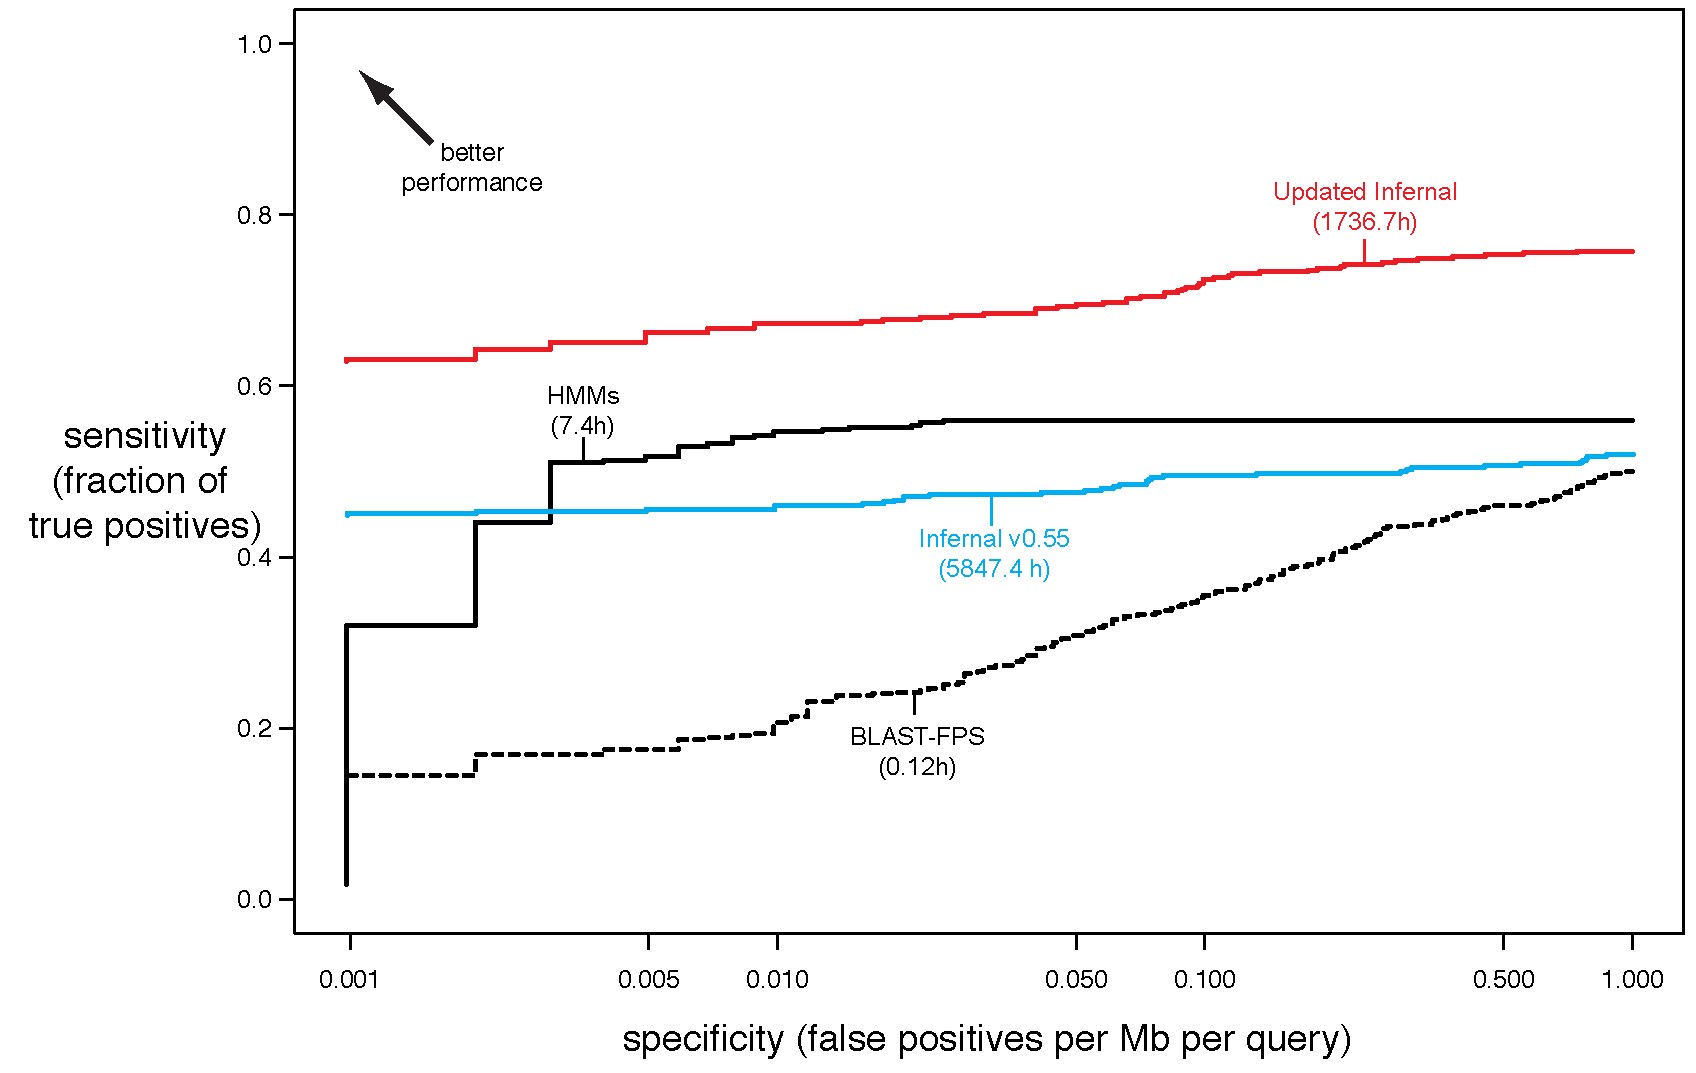
\includegraphics[width=10in]{figs/defense-roc2}}

\vfill 
\end{slide}
%%%%%%%%%%%%%%%%%%%%%%%%%%%%%%%%%%%%%%%%%%%%%%%%%%%%%%%%%%%%%%%%%%%%%%
\begin{comment}
\begin{slide}
\begin{center}
\textbf{Accelerating CM homology search}
\end{center}

\medskip
\small
\begin{itemize}

\item
CM homology search CYK and Inside dynamic programming algorithm \\ scale
$O(LN^2 log N))$ for a database of size $L$ and an RNA of length
$N$

\item Two complementary acceleration heuristic strategies:

\begin{enumerate}
\item 
Decreasing $L$ (prefiltering database) would speed up searches.

\item 
Banded dynamic programming (decreasing $N^2 logN$ part) would speed up searches.

\begin{itemize}
\item 
  HMM banding is lame when there is no primary sequence conservation, \\ which occurs most of the time during searches. 
\item 
  A sequence-independent method would be useful.
\end{itemize}
\end{enumerate}

\end{itemize}

\vfill
\end{slide}
\end{comment}
%%%%%%%%%%%%%%%%%%%%%%%%%%%%%%%%%%%%%%%%%%%%%%%%%%%%%%%%%%%%%%%%%%%%%%%%%%
\begin{slide}
\begin{center}
%\textbf{CMs are much slower than HMMs}
\textbf{CM searches are especially slow for large RNAs}
\medskip

% CM times taken from table 4.2 of my submitted thesis 
% HMM search: viterbi (should be forward), from CPH talk, doubled to 
% match how the table 4.2 times were computed (for both strands of a 1Mb search)
\small
\begin{tabular}{lr|rr|r}
                  &        & \multicolumn{2}{c|}{search (min/Mb)} \\ %\cline{3-4}
                  &        &        & \\
family            & length & HMM    & \textcolor{red}{CM}     & \textcolor{red}{CM/HMM} \\ \hline 
                  &        &        &        & \\
tRNA              & 71     &  0.34  &  \textcolor{red}{27.0}  & \textcolor{red}{79.4}\\
                  &        &        &        & \\
%5S rRNA           & 119    &  0.54  &  \textcolor{red}{26.9}  & \textcolor{red}{49.8}\\
%                  &        &        &        & \\
Lysine riboswitch & 183    &  0.80  & \textcolor{red}{133.2}  & \textcolor{red}{166.7}\\
                  &        &        &        & \\
SRP RNA           & 304    &  1.32  & \textcolor{red}{276.4}  & \textcolor{red}{214.4}\\
                  &        &        &        & \\
RNaseP RNA        & 365    &  1.56  & \textcolor{red}{733.4}  & \textcolor{red}{470.3}\\
                  &        &        &      \\
%SSU rRNA          & 1466   &  0.93 &    - \\
%SSU rRNA          & 1466   &  4.00 & 7660.0&  0.08  & 795.6 \\
%                  &        &        &        &         &  \\
\end{tabular}
\end{center}

\vfill

\end{slide}
%%%%%%%%%%%%%%%%%%%%%%%%%%%%%%%%%%%%%%%%%%%%%%%%%%%%%%%%%%%%%%%%%%%%
\begin{slide}
\begin{center}
\textbf{Why CM homology search is so slow}
\end{center}

\medskip
\small
\begin{itemize}

\item
CM homology search algorithms align/score all subsequences of length
$1..W$ \\ as they scan along the target sequence
looking for high scoring hits
\end{itemize}

\center{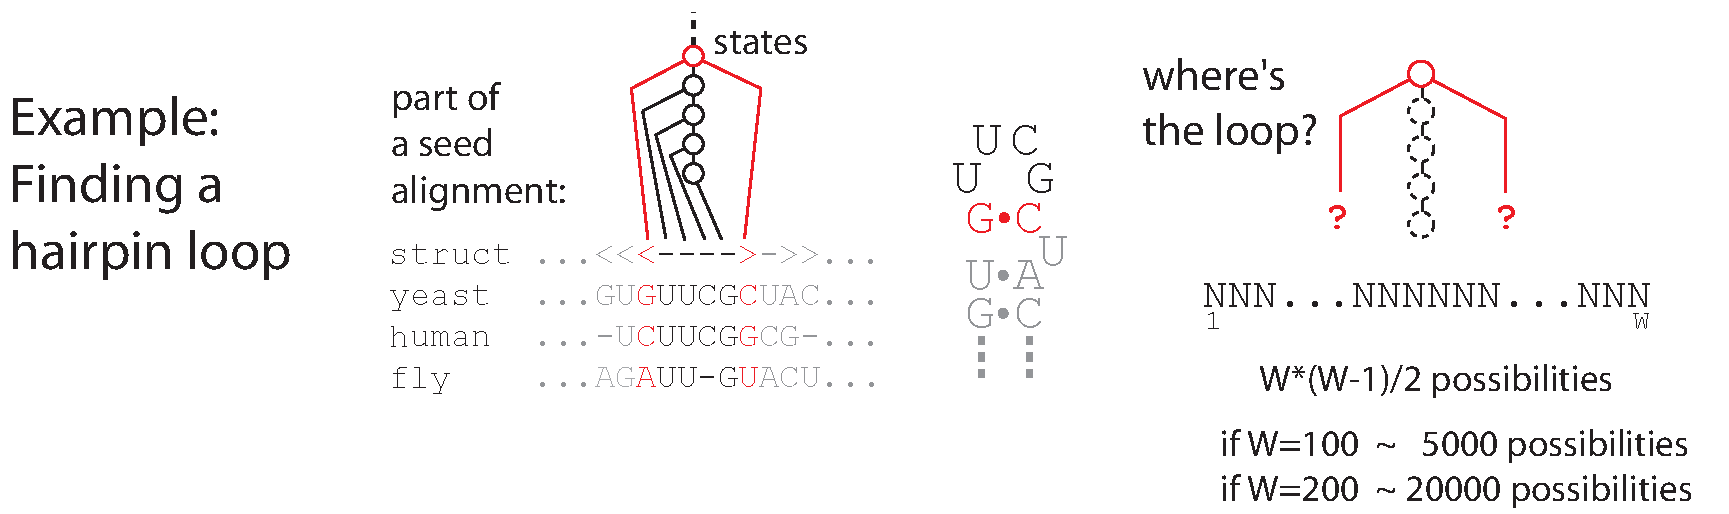
\includegraphics[width=10.4in]{figs/wheresloop}}

  We could save time by restricting the possible loop lengths
  considered.

  {\bf One idea: take advantage of the generative capacity of CMs \\ to generate
  sequences and examine loop length distribution.}

\vfill
\end{slide}
%%%%%%%%%%%%%%%%%%%%%%%%%%%%%%%%%%%%%%%%%%%%%%%%%%%%%%%%%%%%%%%%%%%%%%%%%%
%%%%%%%%%%%%%%%%%%%%%%%%%%%%%%%%%%%%%%%%%%%%%%%%%%%%%%%%%%%%%%%%%%%%%%%%%%
% Slide X: QDB intro
%
\begin{slide}
\begin{center}
\textbf{Query-dependent banding (QDB) strategy}
\end{center}

\tiny
\begin{itemize}
\item
Calculate $\gamma_v(d)$ probability each state $v$ will emit/align to
subsequences of length $d$, for $d = 0..Z$

\begin{tabular}{l|l|l}
\multicolumn{3}{l}{for states $v = M-1$ down to $0$:} \\
$v = $ end state $(E)$: & $\gamma_v(0) = 1$ & \\
                        & $\gamma_v(d) = 0$ & for $d=1$ to $Z$ \\
& & \\
$v = $ bifurcation $(B)$: & $\gamma_v(d) = \sum_{n=0}^{d} \gamma_y(n)
* \gamma_z(d-n)$ & for $d = 0$ to $Z$ \\
& & \\
else ($v = S, P, L, R$): & $\gamma_v(d) = 0$ & for $d=0$ to $(\Delta_v^{L} + \Delta_v^{R} -
1)$ \\
& $\gamma_v(d) = \sum_{y \in C_v} \gamma_y(d-(\Delta_v^{L} + \Delta_v^{R})) * t_v(y) $ 
& for $d = (\Delta_v^{L} + \Delta_v^{R})$ to $Z$ \\
\end{tabular}

\end{itemize}
\center{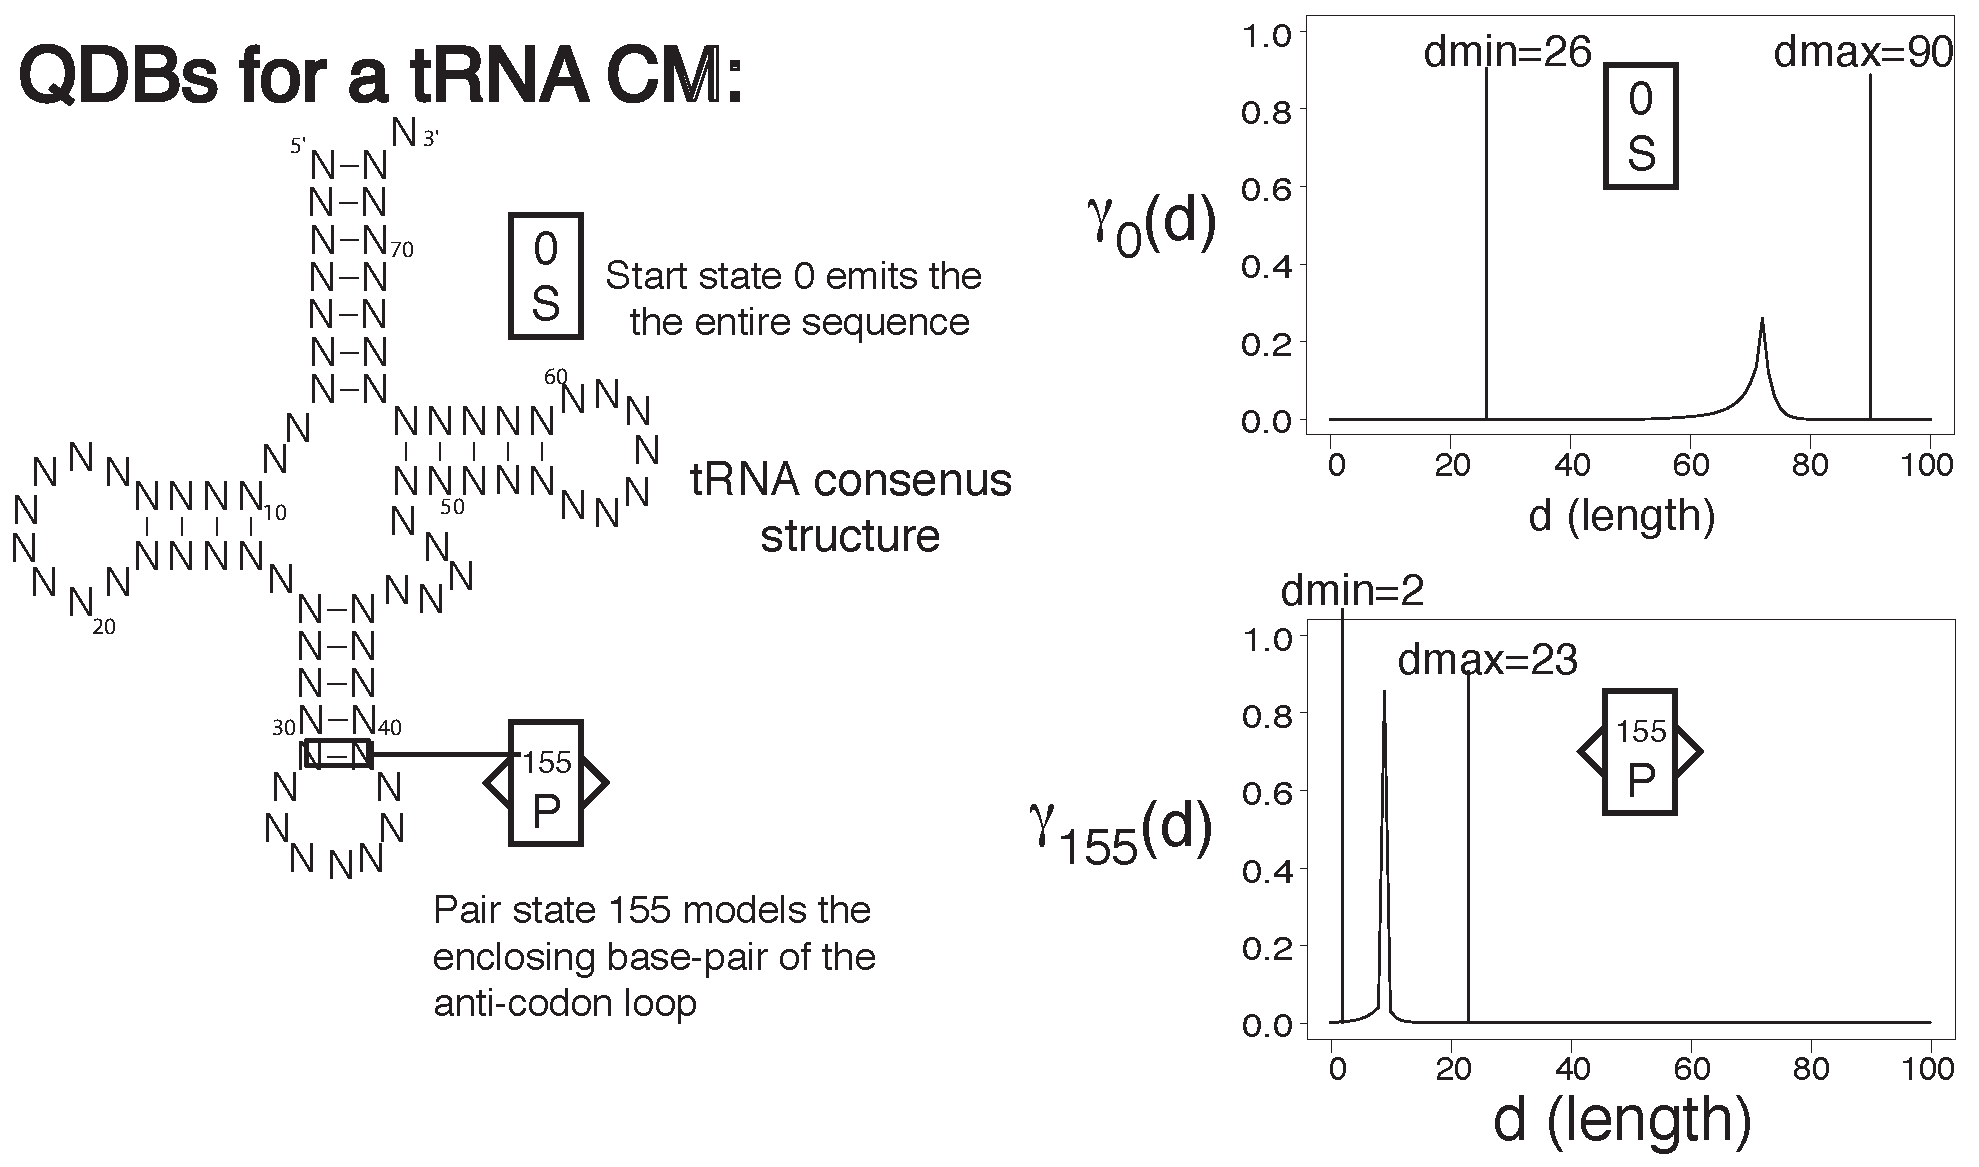
\includegraphics[height=5in]{figs/qdb}}

\vfill
\end{slide}
%%%%%%%%%%%%%%%%%%%%%%%%%%%%%%%%%%%%%%%%%%%%%%%%%%%%%%%%%%%%%%%%%%%%%%%%%%%%%%%%%%%%
\begin{slide}
\begin{center}
\textbf{The $\beta$ parameter controls amount of probability loss}
\end{center}

\begin{minipage}{6in}

\center{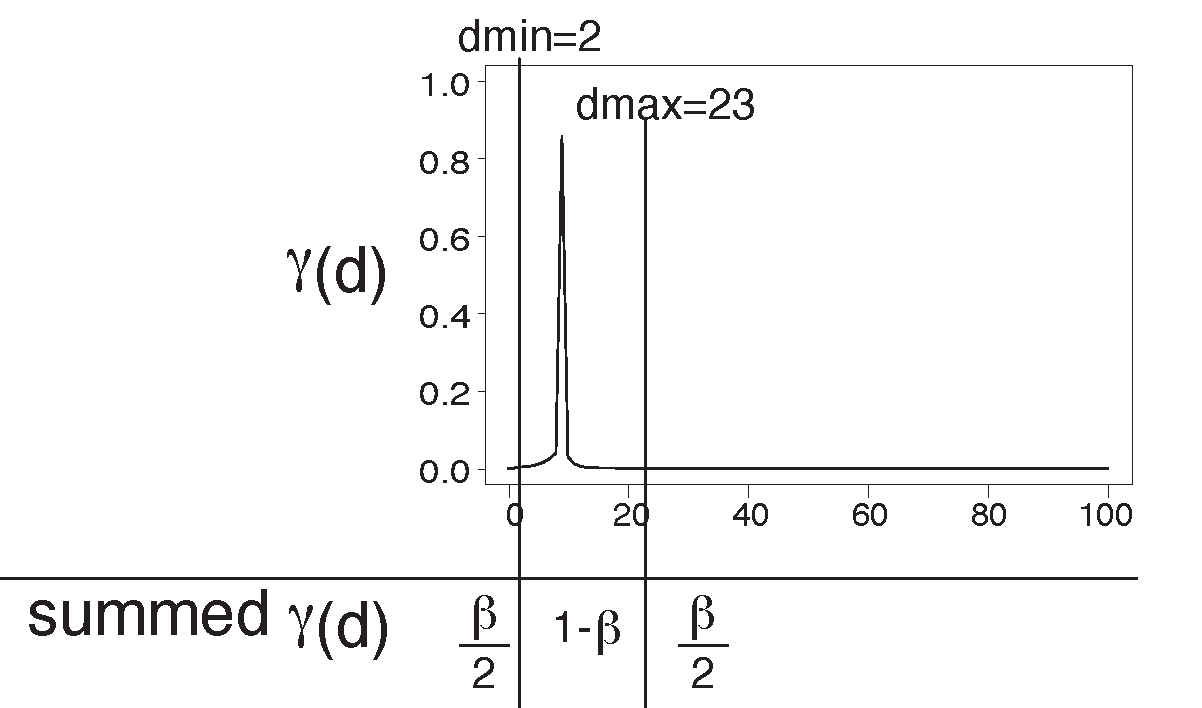
\includegraphics[width=6in]{figs/qdb-beta}}

\vspace{1in}
\begin{itemize} 
\item $\beta$ is typically very small \\
  for example: $0.0000001 (10^{-7})$

\item Higher $\beta$ gives more acceleration \\ but at larger cost to
  accuracy
\end{itemize}

\vspace{1.5in}
\end{minipage}
\begin{minipage}{4in}

\small

\[
   \sum_{d = 0}^{\mbox{dmin} - 1} \gamma(d) < \frac{\beta}{2}
\]

\[
   \sum_{d = \mbox{dmin}}^{\mbox{dmax}} \gamma(d) = 1 - \beta
\]

\[
   \sum_{d = \mbox{dmax} + 1}^{Z} \gamma(d) < \frac{\beta}{2}
\]


\vspace{3in}
\end{minipage}


\end{slide}

%%%%%%%%%%%%%%%%%%%%%%%%%%%%%%%%%%%%%%%%%%%%%%%%%%%%%%
\begin{comment}
\begin{slide}
\begin{center}
\textbf{Choice of probability loss ($\beta$ parameter)}
\end{center}

\small


\center{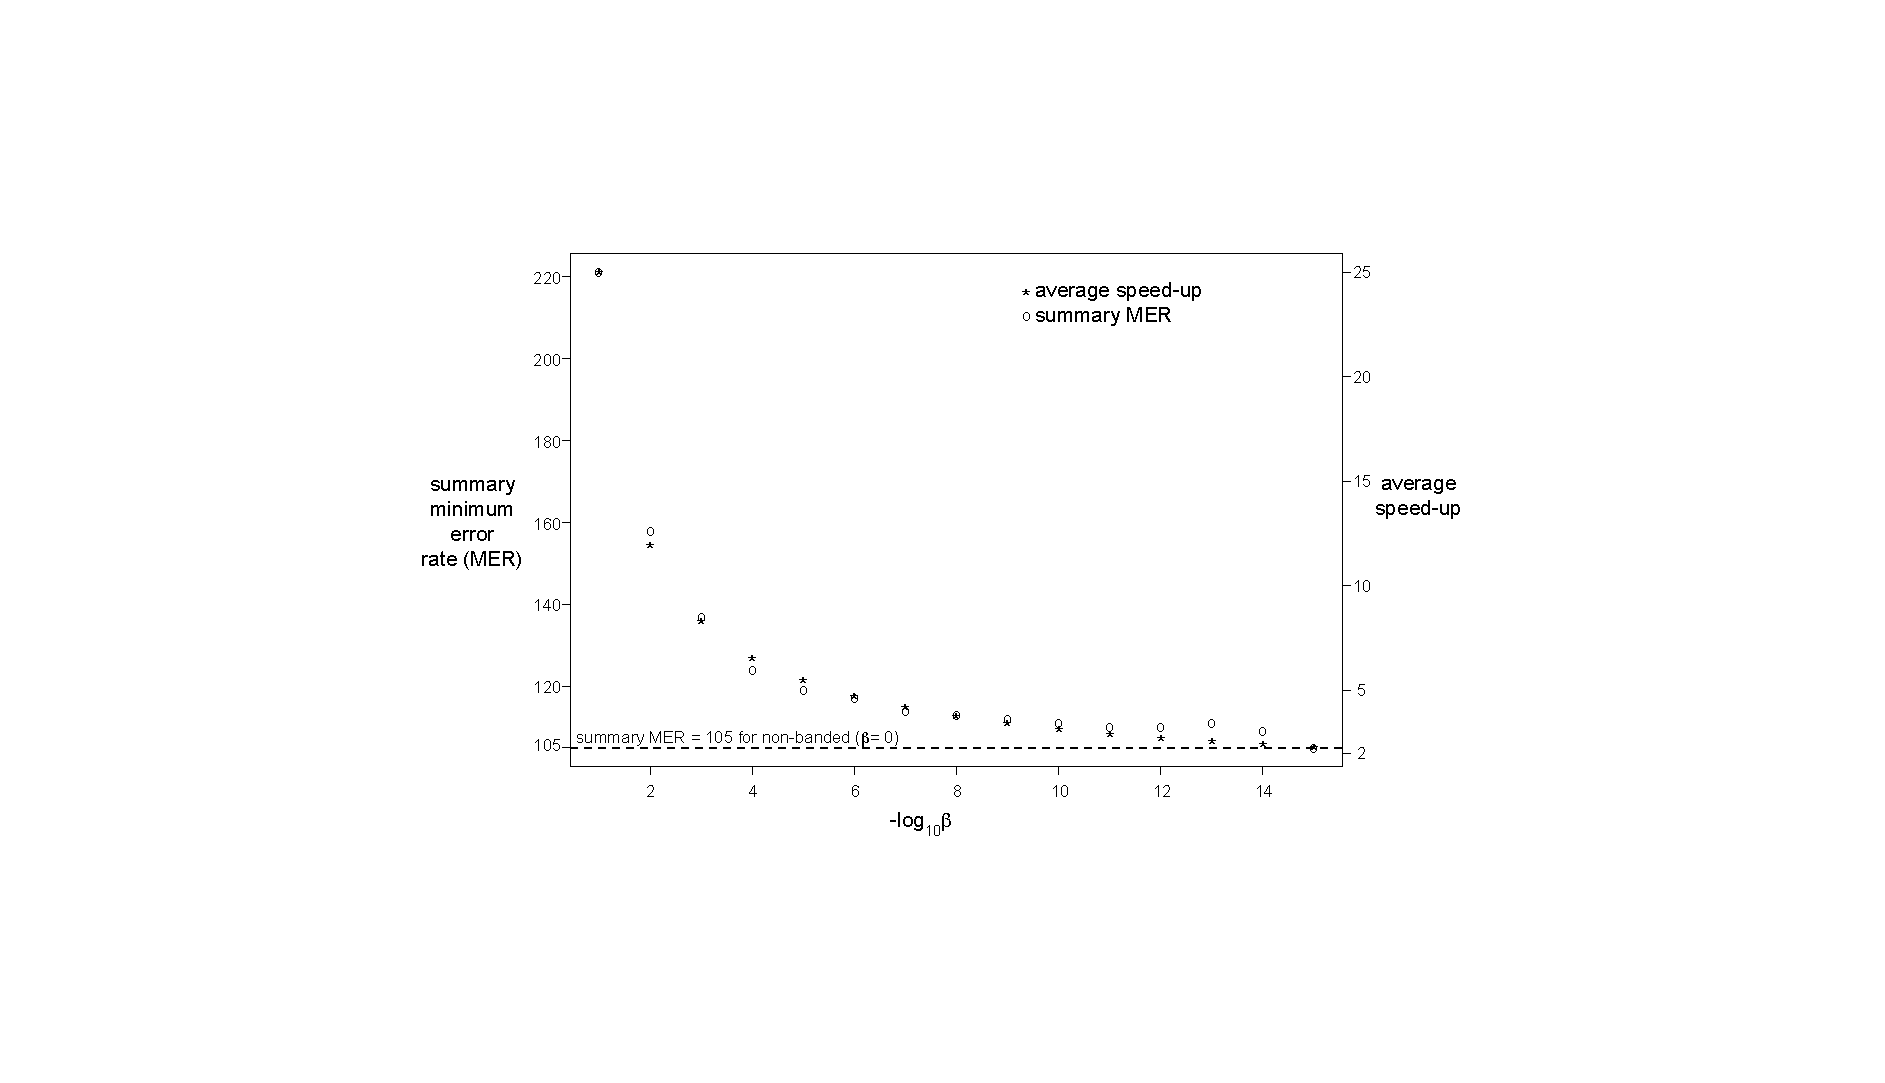
\includegraphics[width=10in]{figs/betavaried}}

\vfill
\end{slide}
\end{comment}
%%%%%%%%%%%%%%%%%%%%%%%%%%%%%%%%%%%%%%%%%%%%%%%%%%%%%%%%
\begin{slide}
\begin{center}
\textbf{Empirical time complexity of CM homology search}
\end{center}

\center{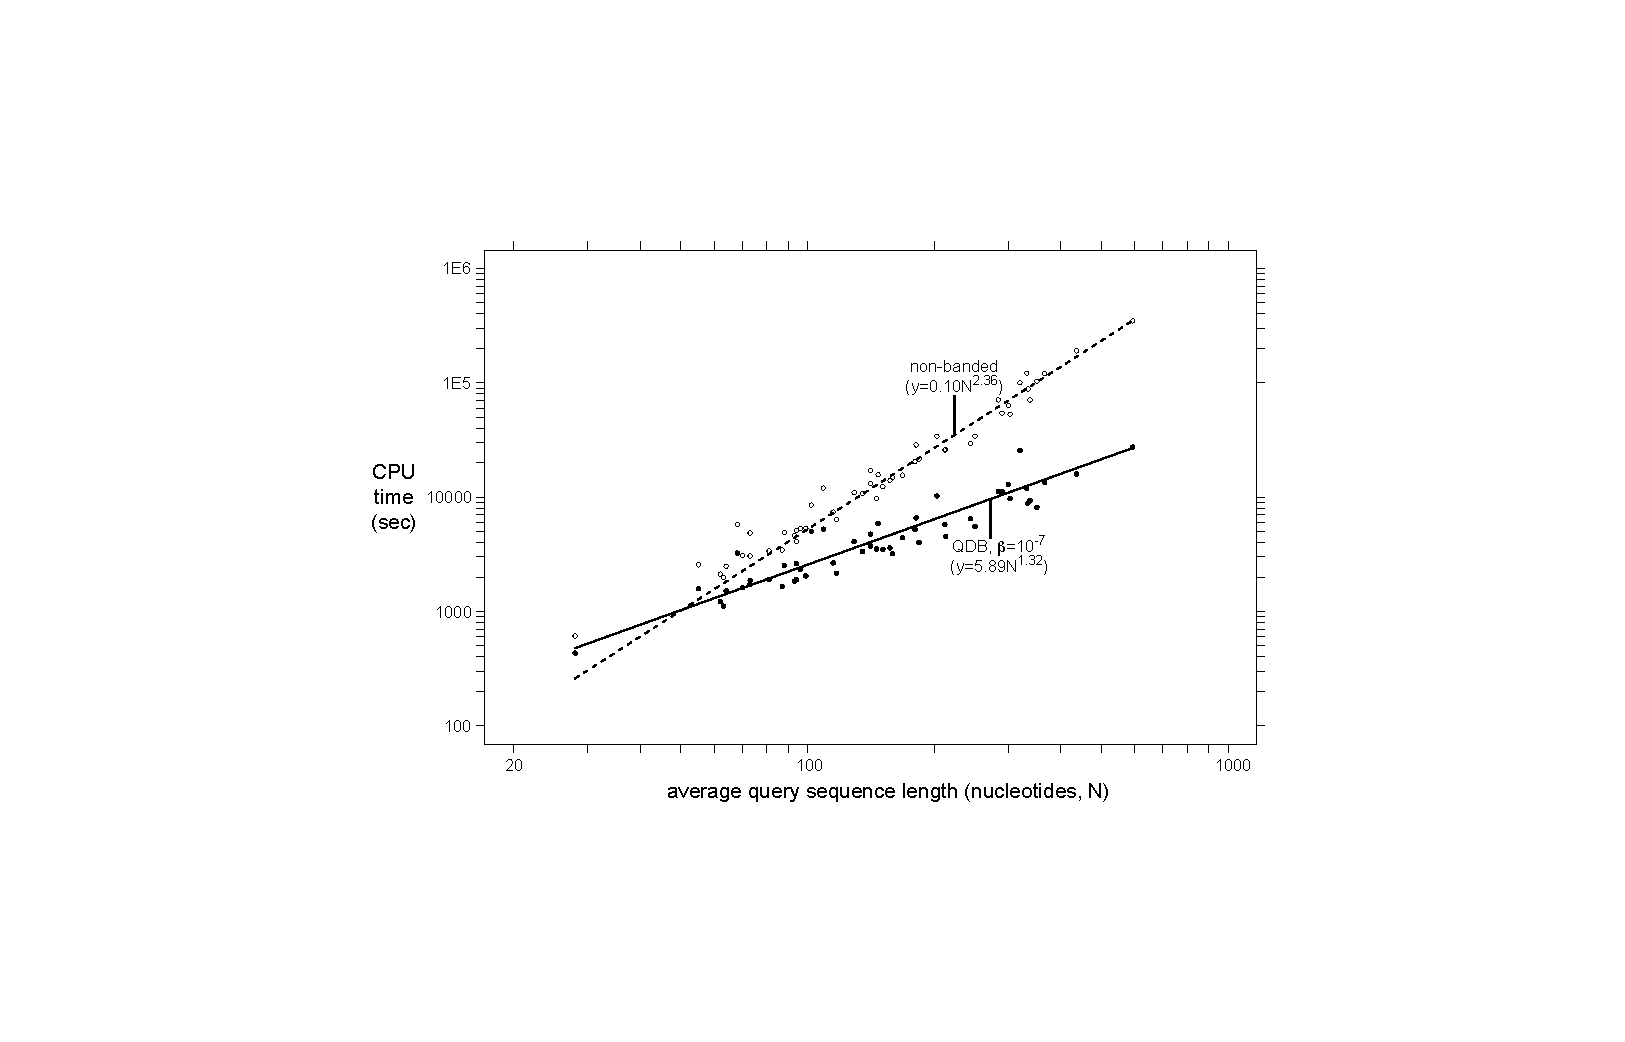
\includegraphics[width=10in]{figs/speedup}}

\vfill
\end{slide}

%%%%%%%%%%%%%%%%%%%%%%%%%%%%%%%%%%%%%%%%%%%%%%%%%%%%%%%%%%%%%%%%%%%%%%%%%%%%%%%%%%%%
\begin{slide}
\begin{center}
\textbf{QDB sacrifices very little sensitivity and gives 6-fold speedup}
\end{center}

\center{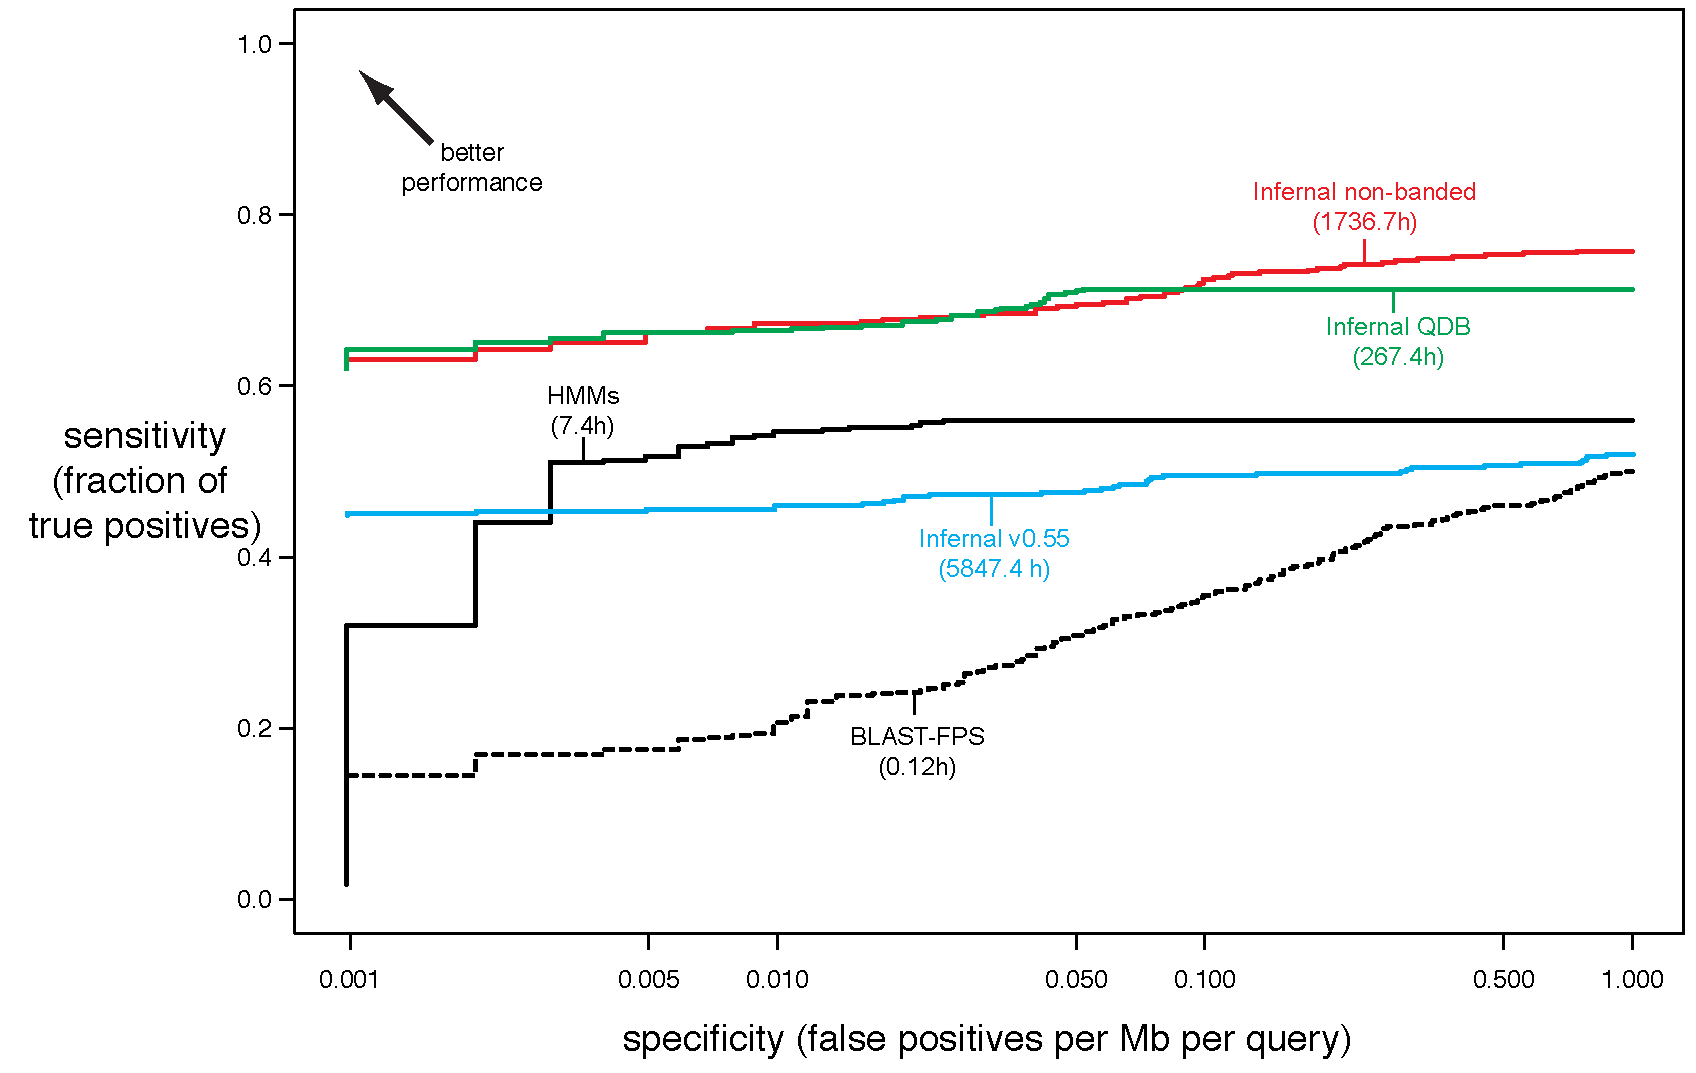
\includegraphics[width=10in]{figs/defense-roc3}}

\vfill
\end{slide}

%%%%%%%%%%%%%%%%%%%%%%%%%%%%%%%%%%%%%%%%%%%%%%%%%%%%%%%%%%%%%%%%%%%%%%%%%%%%%%%%%%%%
\begin{slide}
\begin{center}
\textbf{CM homology searches are still slow}
\end{center}

%timings: QDB, took regular CM times and divided by speedup
%         for QDB paper table 5. For SSU, ran cmsearch 1.0 --forecast
\small
\begin{center}
\small
\begin{tabular}{lr|rr|r|r}
                  &        & \multicolumn{2}{c|}{search (min/Mb)} & \multicolumn{2}{c}{}\\ \cline{3-4}
%                  &        &        &        &            &         \\
                  &        &        &        & \textcolor{mygreen}{QDB}  & non-banded        \\
family            & length & HMM    & \textcolor{mygreen}{QDB CM} & \textcolor{mygreen}{CM/HMM} & CM/HMM  \\ \hline
                  &        &        &        &            &         \\
tRNA              & 71     &  0.34  &  \textcolor{mygreen}{9.6}   & \textcolor{mygreen}{28.2} & \textcolor{black}{79.4}\\
                  &        &        &        &            &         \\
%5S rRNA           & 119    &  0.54  &  \textcolor{mygreen}{9.1}   & \textcolor{mygreen}{16.9} & \textcolor{black}{49.8}\\
%                  &        &        &        &            &         \\
Lysine riboswitch & 183    &  0.80  &  \textcolor{mygreen}{33.8}  & \textcolor{mygreen}{42.3} & \textcolor{black}{166.7}\\
                  &        &        &        &            &         \\
SRP RNA           & 304    &  1.32  &  \textcolor{mygreen}{50.5}  & \textcolor{mygreen}{38.3} & \textcolor{black}{214.4}\\
                  &        &        &        &            &         \\
RNaseP RNA        & 365    &  1.56  &  \textcolor{mygreen}{81.6}  & \textcolor{mygreen}{52.3} & \textcolor{black}{470.3}\\
                  &        &        &        &            &         \\
\end{tabular}
\end{center}

\vfill

\end{slide}
%%%%%%%%%%%%%%%%%%%%%%%%%%%%%%%%%%
\begin{slide}

\begin{center}
\textbf{Filtering as a complementary acceleration strategy}
\end{center}

%\item
%  Query-dependent banding (QDB) accelerates
%  homology search six-fold at a negligible cost to sensitivity
\small
\begin{itemize}
\item
  Main idea: search database with faster method first, hits above some threshold \\ survive the filter and are searched with the slow CM.
%\item
%  Goal of filtering: Maximal speedup with minimal loss of sensitivity
%\item
%  Rfam uses a BLAST filter at an unknown cost to sensitivity
%\item
%  \emph{tRNAscan-SE}: filters database using tRNA-specific heuristics to find tRNAs
\item
  Weinberg and Ruzzo developed HMM filters for faster searches
\item
  Others have also worked on this (Sun \& Buhler, 2008; Zhang \&
  Bafna, 2006)
\end{itemize}

\center{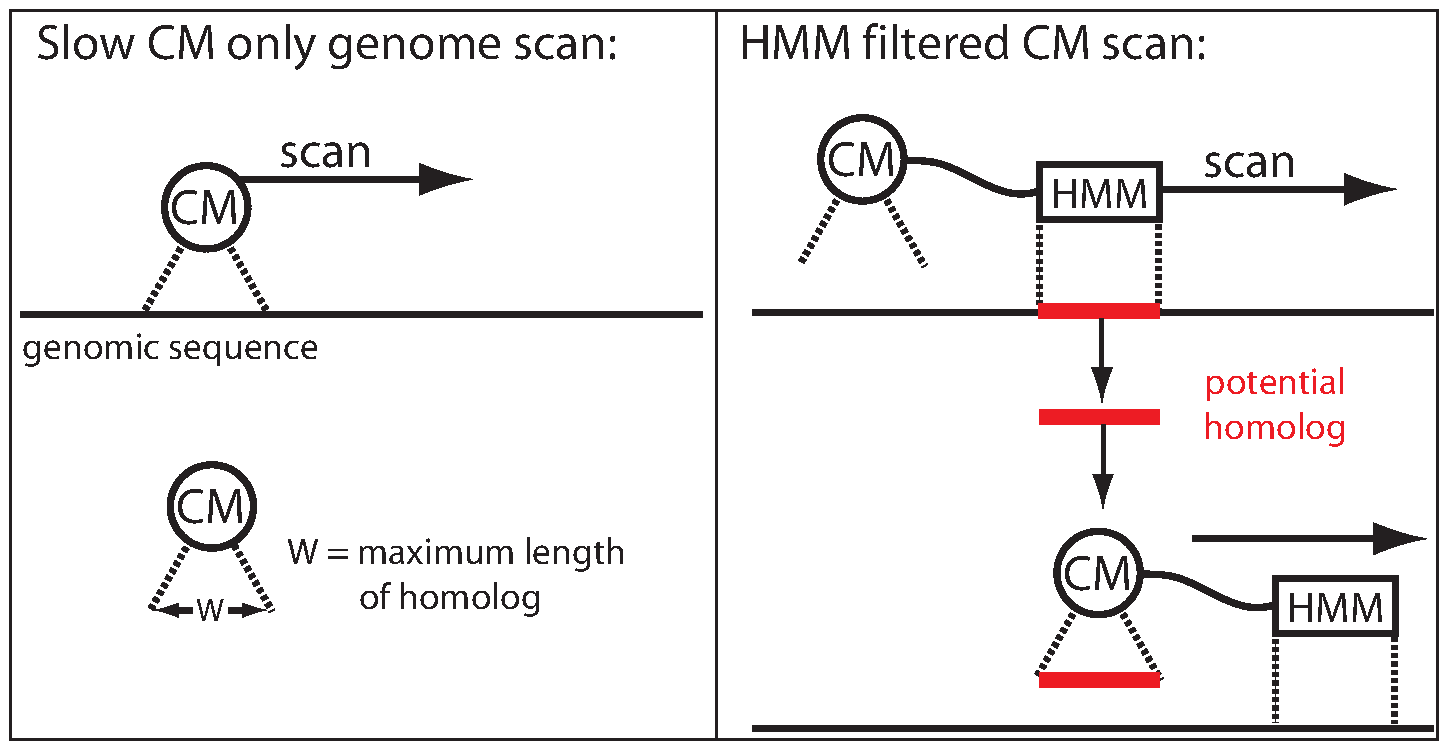
\includegraphics[width=8in]{figs/filter}}
\vfill

\end{slide}
%%%%%%%%%%%%%%%%%%%%%%%%%%%%%%%%%%%%%%%%%%%%%%%%%%%%%%%%%%%%%%%%%%%%%%%%%%
%%%%%%%%%%%%%%%%%%%%%%%%%%%%%%%%%%
\begin{slide}

\begin{center}
\textbf{HMM filters achieve 10-fold speedup at very small cost to accuracy}
\end{center}

\center{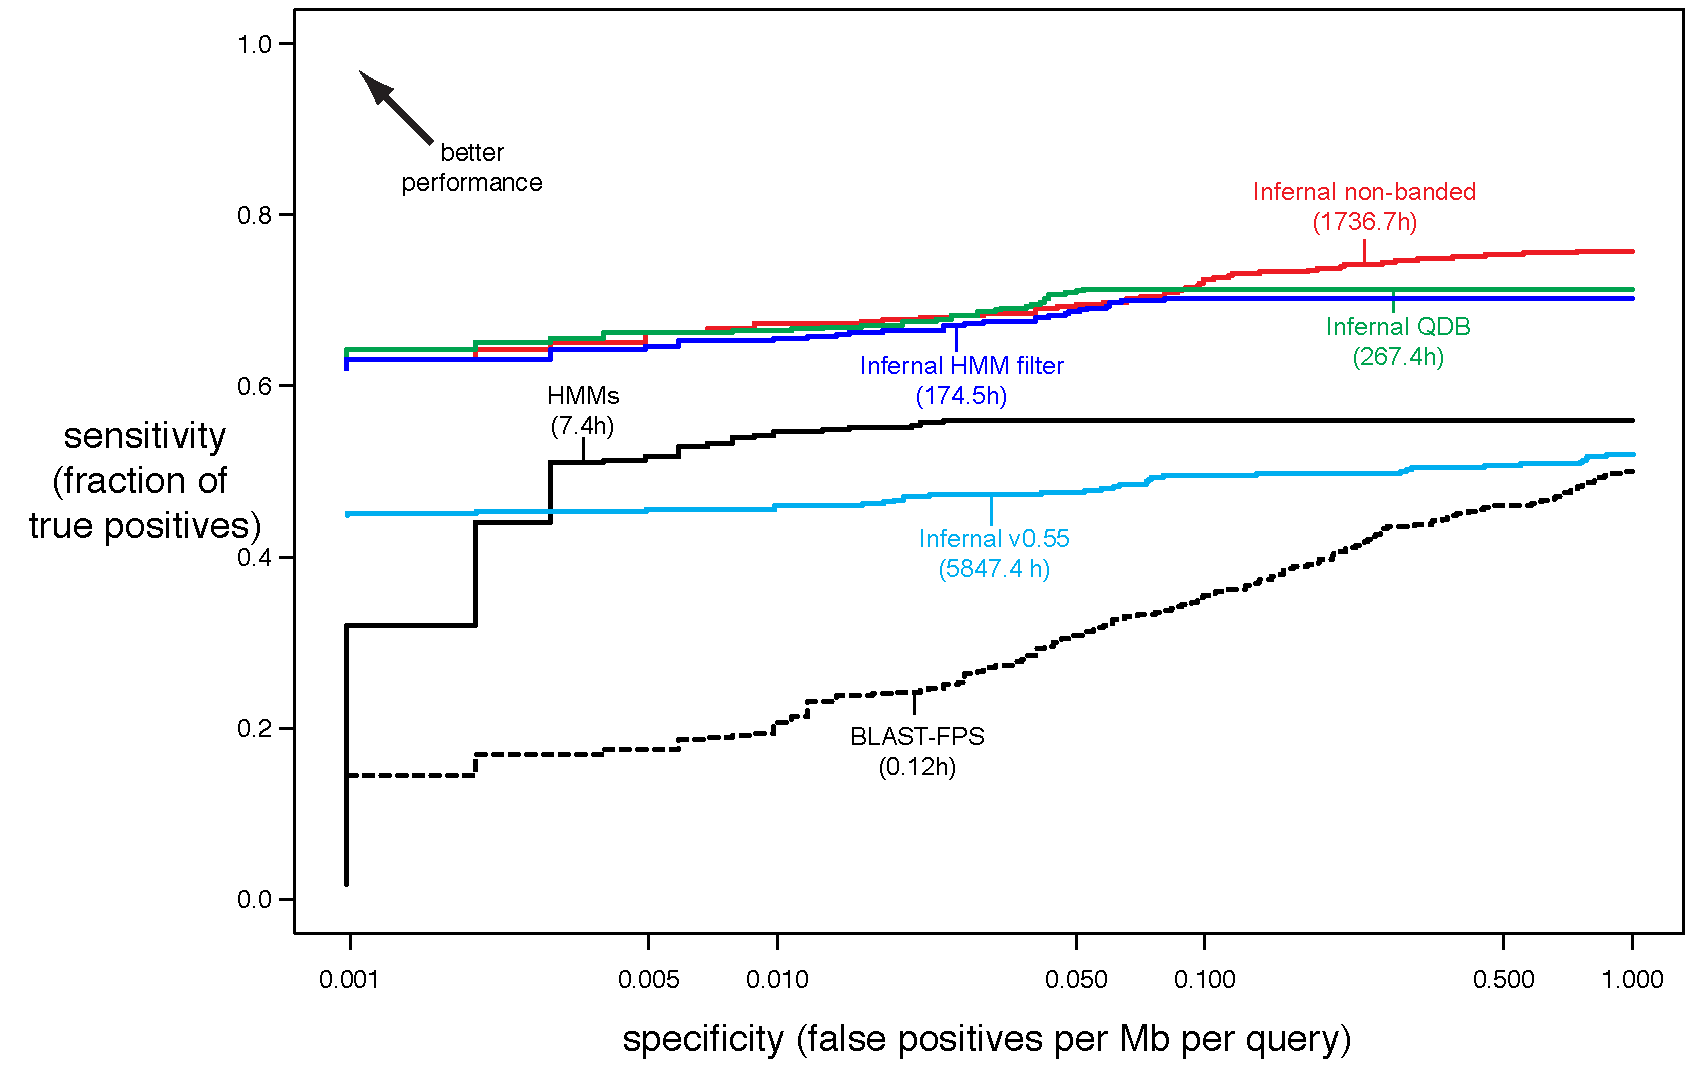
\includegraphics[width=10in]{figs/defense-roc4}}

\vfill

\end{slide}
%%%%%%%%%%%%%%%%%%%%%%%%%%%%%%%%%%
\begin{slide}

\begin{center}
\normalsize
\textbf{Combining QDB and HMM filters yields greater acceleration}

\small
%
The more powerful, slower Inside algorithm is used post-filtering.

Infernal is now 100-fold faster and significantly more sensitive than v0.55.
%

\end{center}

\center{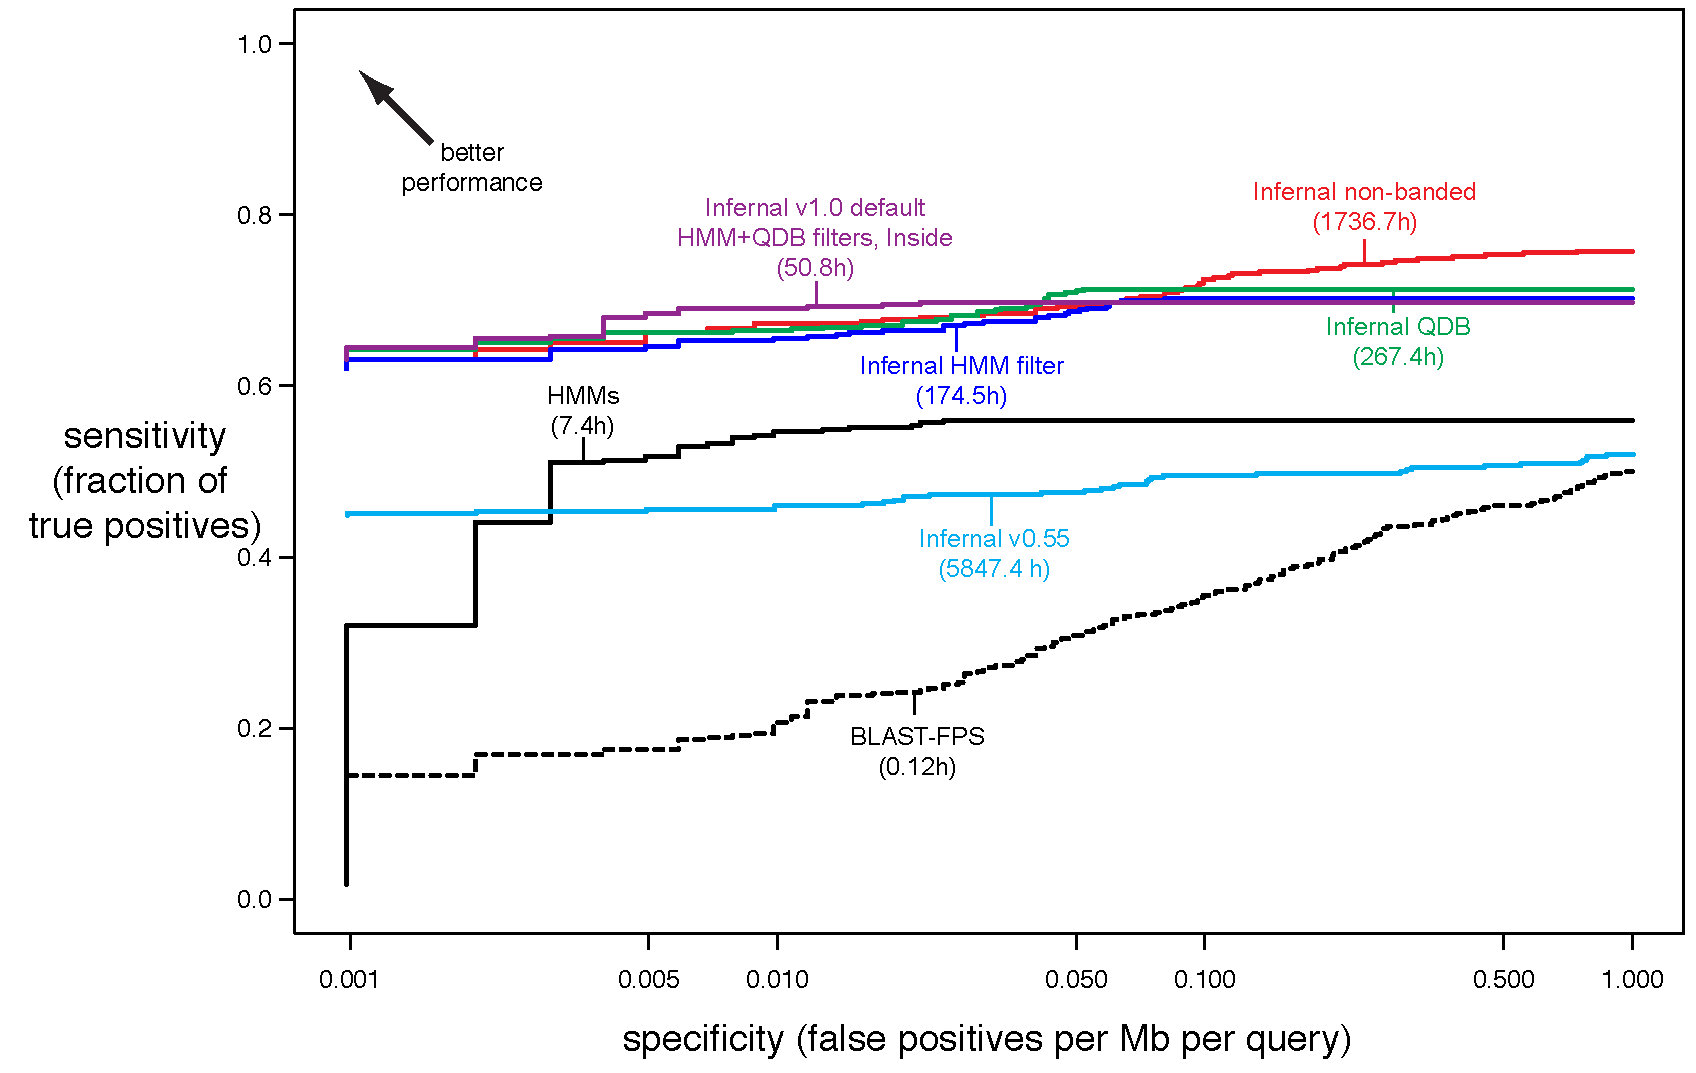
\includegraphics[width=10in]{figs/defense-roc5}}

\vfill

\end{slide}
%%%%%%%%%%%%%%%%%%%%%%%%%%%%%%%%%%
\begin{slide}
\begin{center}

  \textbf{CMs are now nearly as fast as HMMs (usually)}
\end{center}


\small
\begin{center}
\small
\begin{tabular}{lr|rr|r|r}
                  &        & \multicolumn{2}{c|}{search (min/Mb)} & \multicolumn{2}{c}{}\\ \cline{3-4}
                  &        &        &        &            &         \\

                  &        &        & \textcolor{mypurple}{HMM+QDB}    & \textcolor{mypurple}{HMM+QDB}  & \\
                  &        &        & \textcolor{mypurple}{filtered}   & \textcolor{mypurple}{filtered}& non-banded        \\
family            & length & HMM    & \textcolor{mypurple}{CM}     & \textcolor{mypurple}{CM/HMM} & CM/HMM  \\ \hline
                  &        &        &        &            &         \\
tRNA              & 71     &  0.34  &  \textcolor{mypurple}{8.8}   & \textcolor{mypurple}{25.9} & \textcolor{black}{79.4}\\
                  &        &        &        &            &         \\
Lysine riboswitch & 183    &  0.80  &  \textcolor{mypurple}{2.2}   & \textcolor{mypurple}{2.8}  & \textcolor{black}{166.7}\\
                  &        &        &        &            &         \\
SRP RNA           & 304    &  1.32  &  \textcolor{mypurple}{6.0}   & \textcolor{mypurple}{4.5} & \textcolor{black}{214.4}\\
                  &        &        &        &            &         \\
RNaseP RNA        & 365    &  1.56  &  \textcolor{mypurple}{1.8}   & \textcolor{mypurple}{1.2} & \textcolor{black}{470.3}\\
                  &        &        &        &            &         \\

\end{tabular}
\end{center}

\vfill

\end{slide}
%%%%%%%%%%%%%%%%%%%%%%%%%%%%%%%%%%%%%%%%%%%%%%%%%%%%%%%%%%%%%%%%%%%%%%%%%%
\begin{slide}
\begin{center}
\textbf{Structural RNA alignment using CMs}
\end{center}
\medskip

\small
\begin{itemize}
%  \item Finding RNAs in an organism's genome is informs us about the
%    organism.
%    Collecting and analyzing many homologous RNAs from different
%    genomes can inform us about the RNA family:
  \item CMs can also be used to create structural alignments of
    homologous RNAs.
  \item Given known homologs, place homologous residues in the same columns.
\end{itemize}

\center{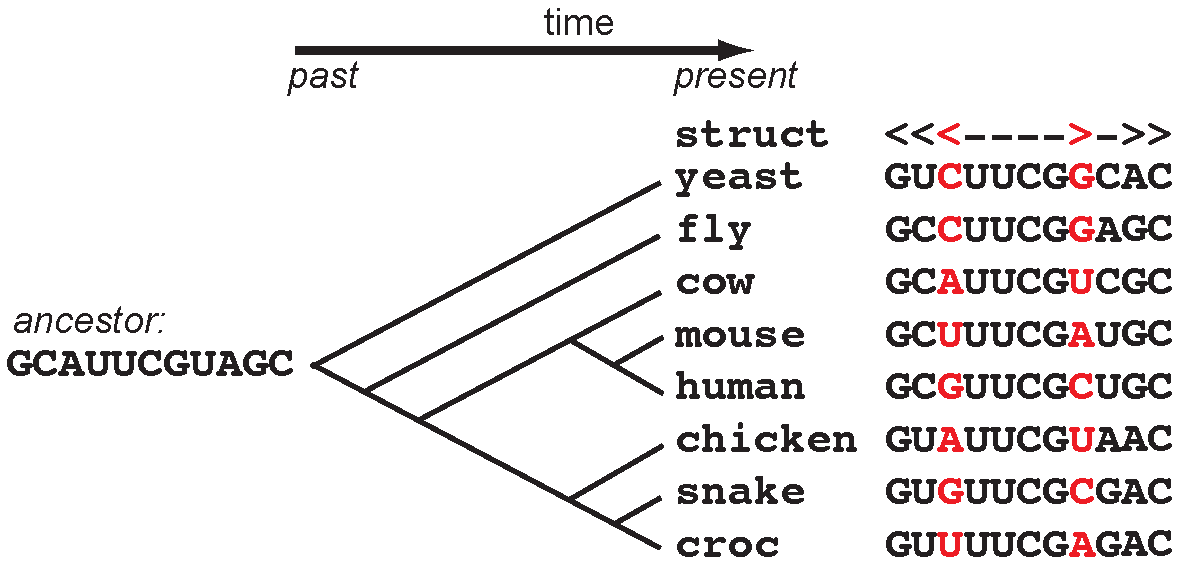
\includegraphics[width=5in]{figs/tree-and-aln}}

\begin{itemize}
\item Alignments of SSU rRNA have commonly been used for phylogenetic inference.

%\begin{itemize}
%  \item RNA alignments have several important applications:
%    \begin{itemize}
%      \item structural inference
%      \item lead to functional hypotheses
%      \item inference of evolutionary history (phylogenetic inference)
%    \end{itemize}
%  \item One RNA in particular has traditionally been used heavily for
%    \\ phylogenetic inference: 

%\item Alignments of SSU rRNA have commonly been used for phylogenetic inference.

\item However, CM alignment is too slow for SSU alignment.
   \\ Aligning a single SSU sequence takes more than 20
    minutes.
\end{itemize}
\vfill
\end{slide}
%%%%%%%%%%%%%%%%%%%%%%%%%%%%%%%%%%%%%%%%%%%%%%%%%%%%%%%%%%%%%%%%%%%%%%
\begin{slide}
\begin{center}

\textbf{Small subunit ribosomal RNA and the tree of life}
\end{center}
\medskip
\begin{minipage}{5.2in}
\small

\begin{itemize}
\item
1977 - Carl Woese decided to classify all living things phylogenetically
\item
needed ``\emph{a molecule of appropriately broad distribution}'' for
comparative analysis
\item
SSU rRNA was chosen
\begin{itemize}
  \item
    universally distributed
  \item
    highly conserved 
  \item
    large enough to provide sufficient data% (1500-1800 nt)
%  \item
%    readily isolated
\end{itemize}
\end{itemize}

\vspace{2.7in}
\end{minipage}
\hspace{0.1in}
\begin{minipage}{5.5in}
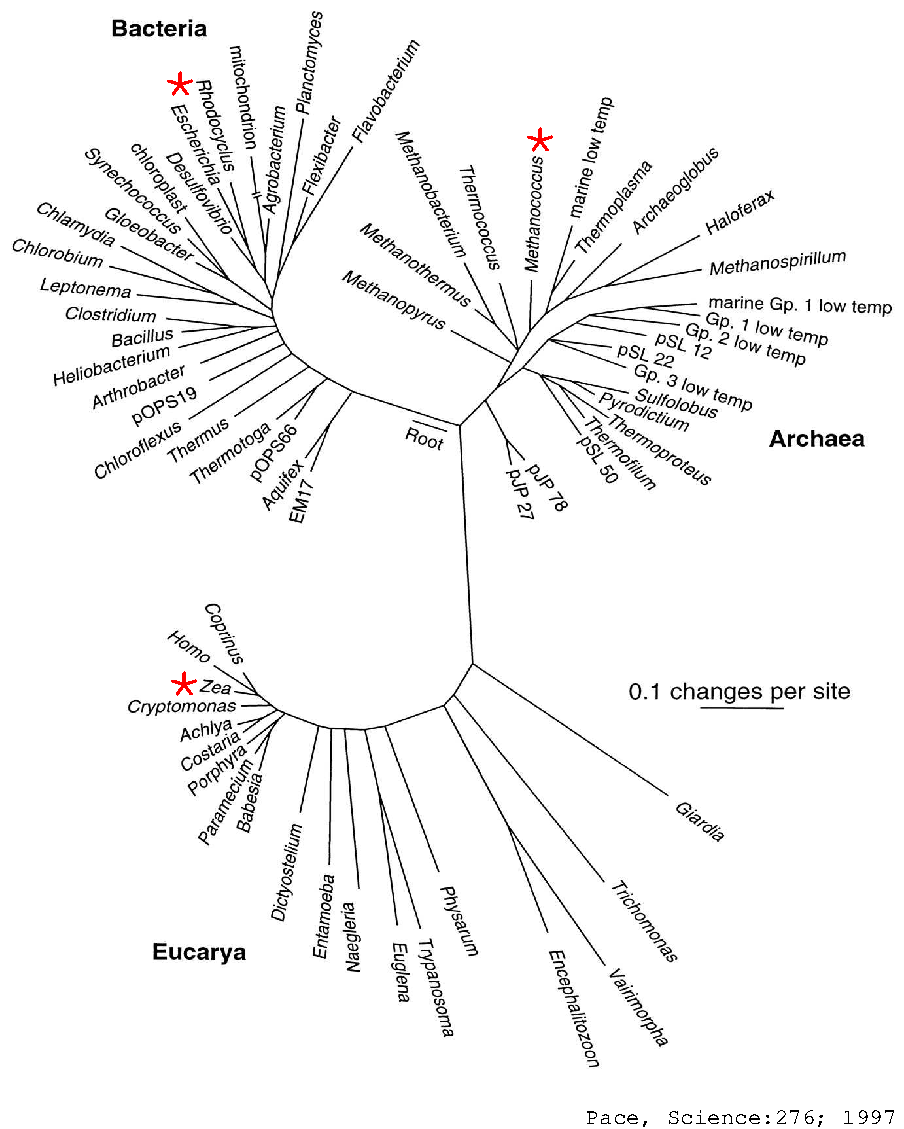
\includegraphics[width=5.5in]{figs/bigtol}
%\vspace{1.5in}
\end{minipage}  

\end{slide}

%%%%%%%%%%%%%%%%%%%%%%%%%%%%%%%%%%%%%%%%%%%%%%%%%%%%%%%%%%%%%%%%%%%%%%%%%%
%Slide 2 - SSU rRNA is very well conserved across all three domains
\begin{slide}
\begin{center}

\textbf{Universal structural conservation of SSU rRNA}
\end{center}
\vspace{0.5in}
\small
\hspace{0.75in}
\emph{Escherichia coli}
\hspace{1.2in}
\emph{Methanococcus vannielii}
\hspace{1.2in}
\emph{Zea mays}

\begin{center}
%\includegraphics[height=4.6in]{figs/ecoli_16S}
%\includegraphics[height=4.6in]{figs/mvan_16S}
%\includegraphics[height=4.6in]{figs/zmays_16S}
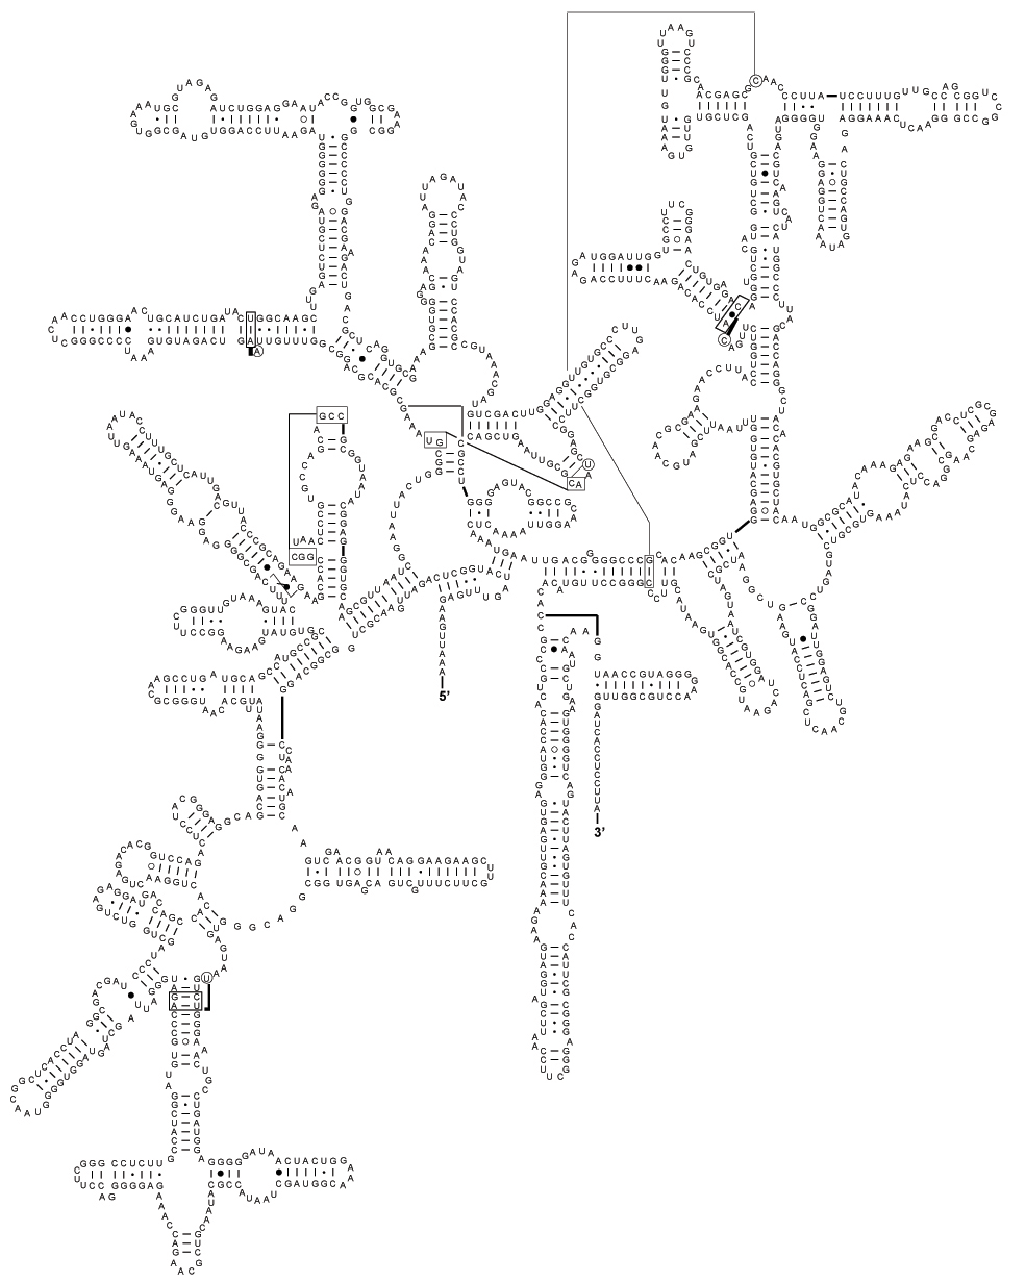
\includegraphics[height=4.45in]{figs/ecoli_16S_man}
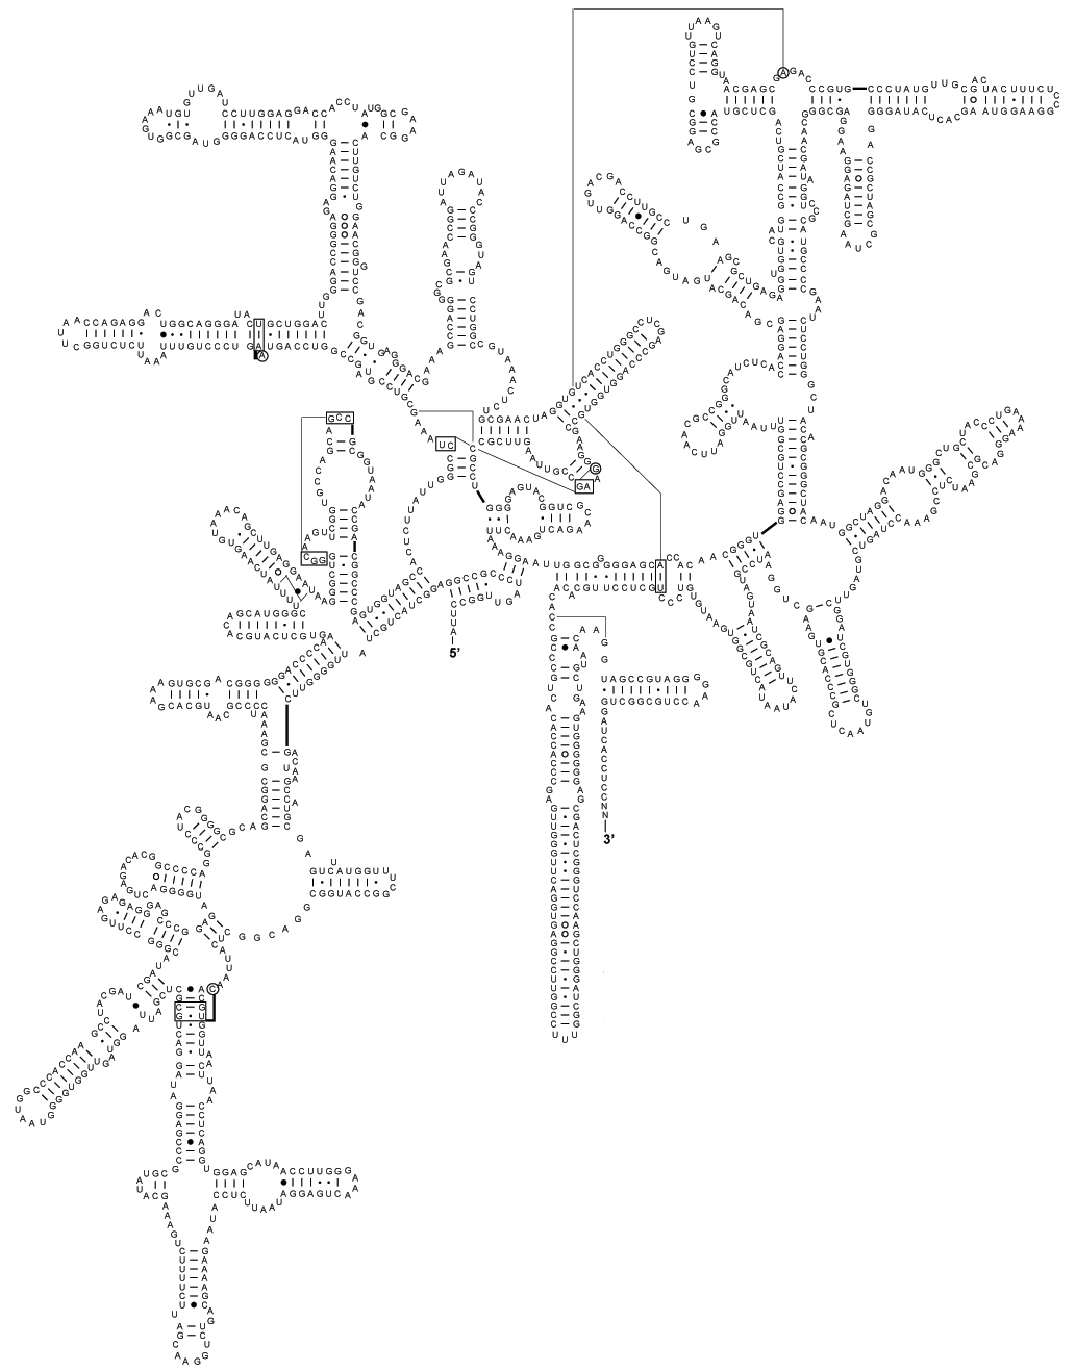
\includegraphics[height=4.45in]{figs/mvan_16S_man}
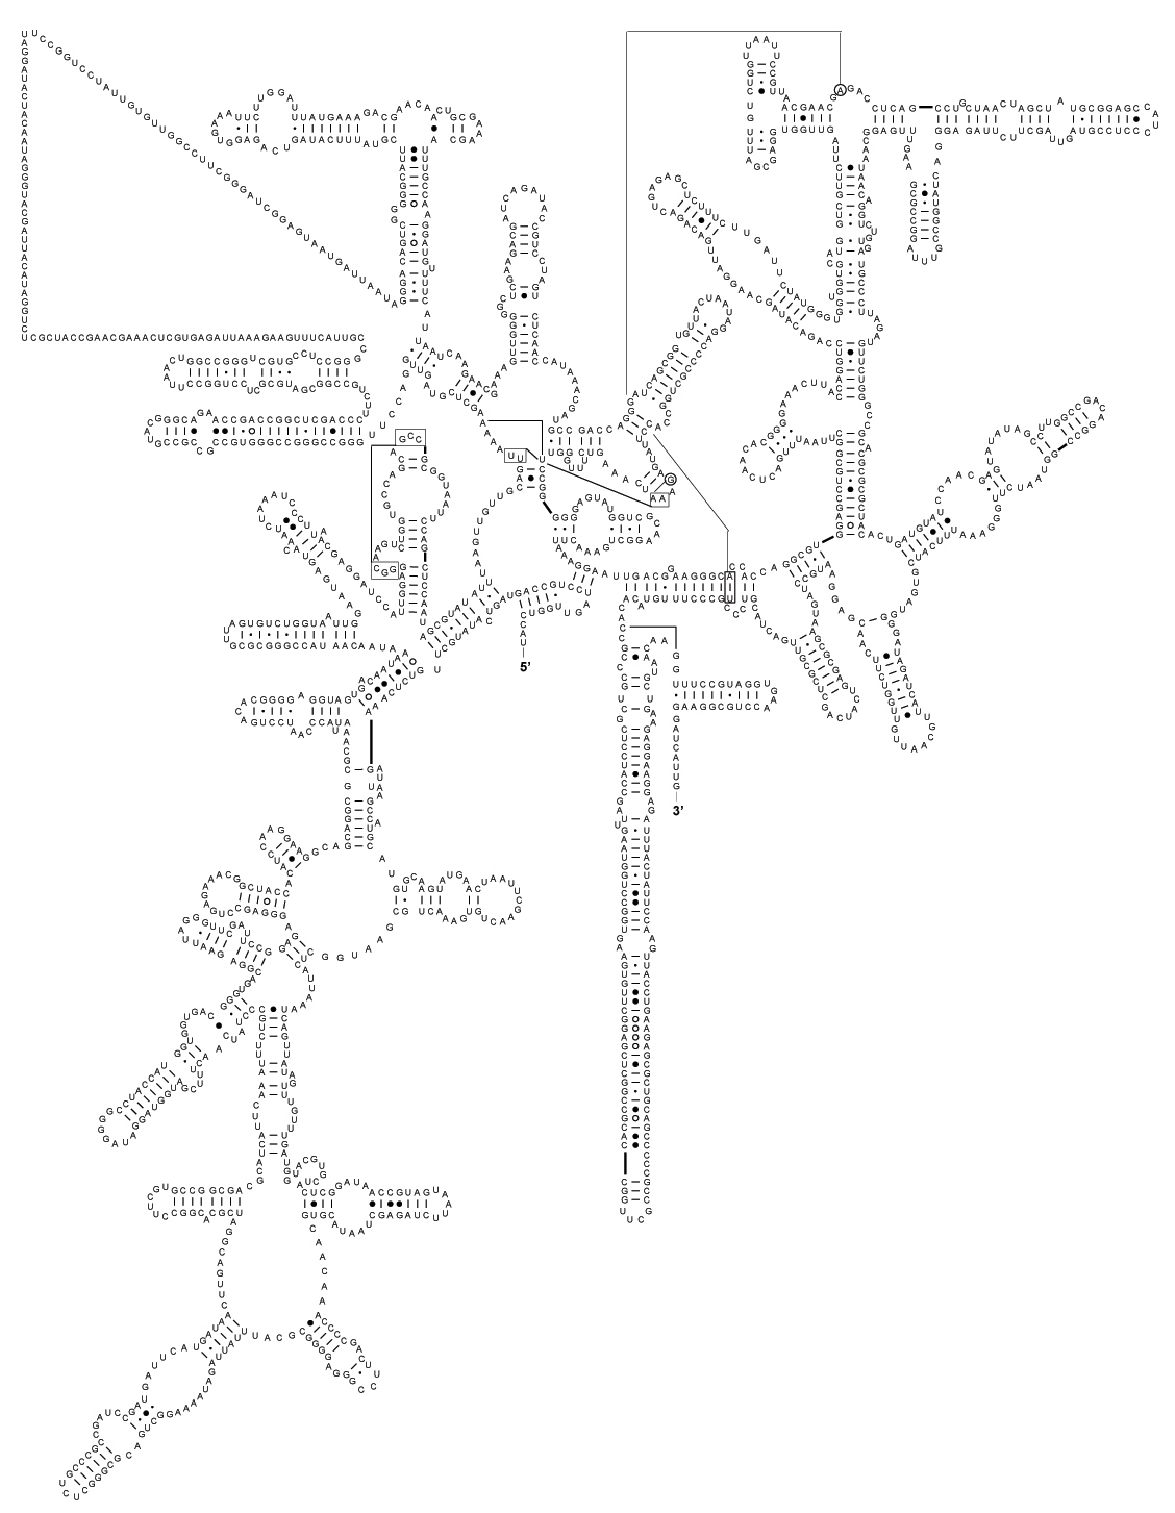
\includegraphics[height=4.45in]{figs/zmays_16S_man}
\end{center}

\begin{flushright}
\tiny{\texttt{Secondary structure diagrams from:}} \\
\tiny{\texttt{URL:http://www.rna.ccbb.utexas.edu/}}
\end{flushright}
%should this slide have a tree of life? if not where should it go?
\vfill
\end{slide}

%%%%%%%%%%%%%%%%%%%%%%%%%%%%%%%%%%%%%%%%%%%%%%%%%%%%%%%%%%%%%%%%%%%%%%%%%%
%Slide 2 - SSU rRNA is very well conserved across all three domains
\begin{slide}
\begin{center}

%\textbf{Universal sequence conservation of SSU rRNA}
\textbf{Sequence conservation in SSU rRNA}
\end{center}
\vspace{0.5in}
\small
\hspace{1.5in}
\underline{bacteria}
\hspace{2.2in}
\underline{archaea}
\hspace{2.2in}
\underline{eukarya}

\begin{center}
%\includegraphics[height=4.6in]{figs/ecoli_16S}
%\includegraphics[height=4.6in]{figs/mvan_16S}
%\includegraphics[height=4.6in]{figs/zmays_16S}
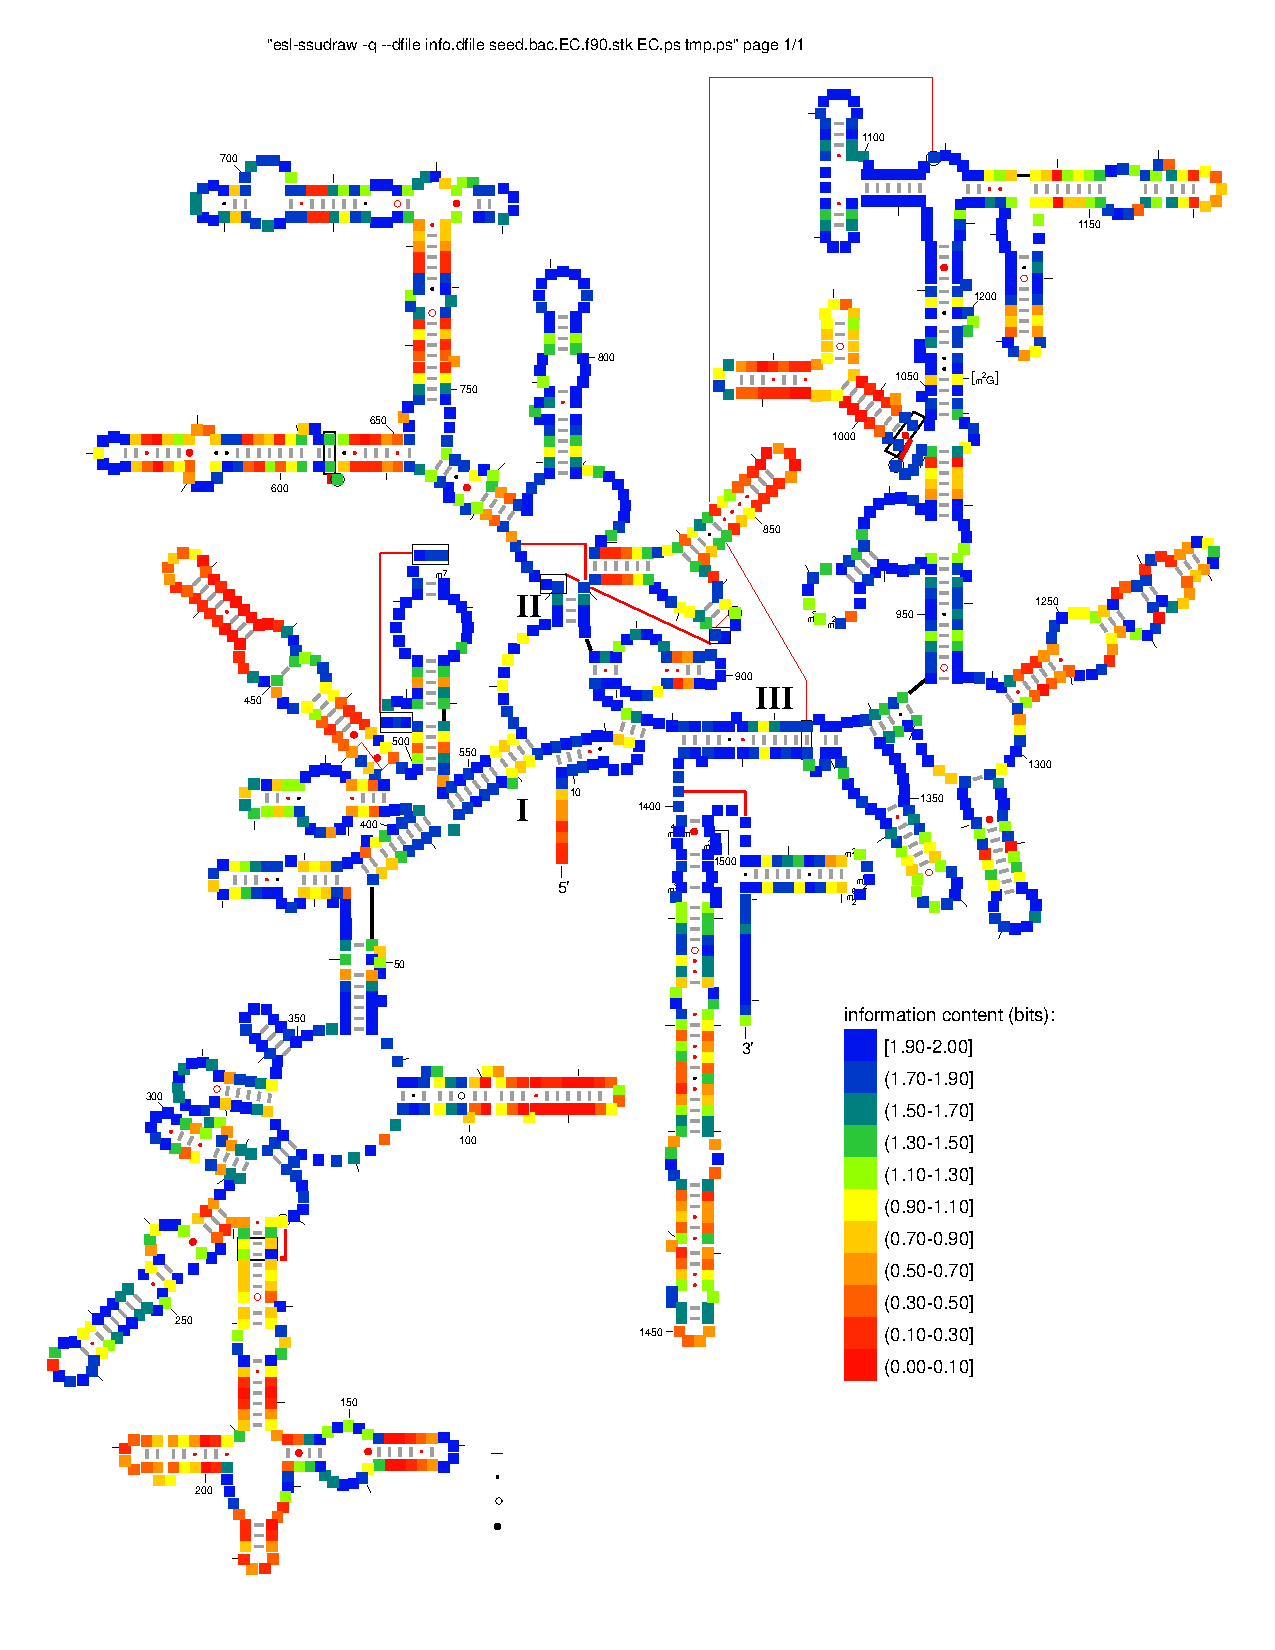
\includegraphics[height=4.45in]{figs/bac_info_heat}
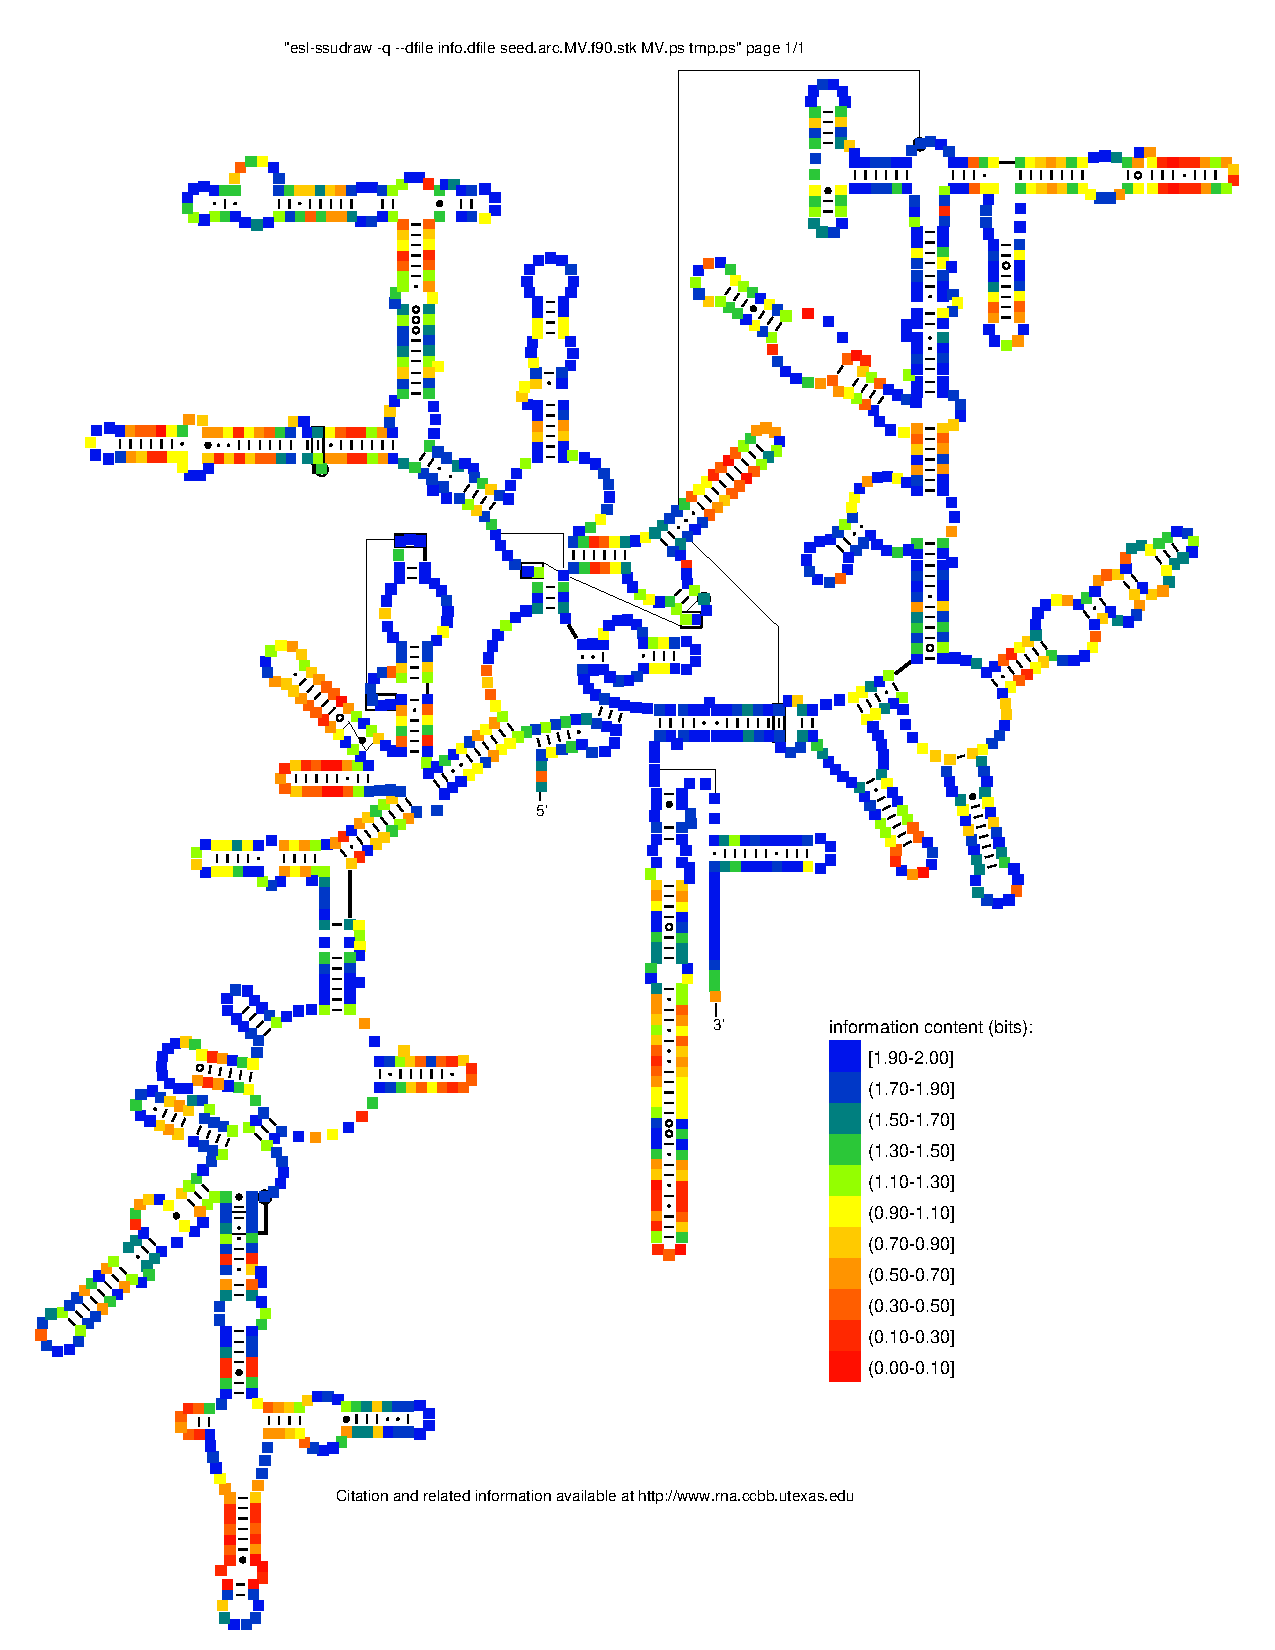
\includegraphics[height=4.45in]{figs/arc_info_heat}
\includegraphics[height=4.45in]{figs/euk_info_heat}
\end{center}

\begin{flushright}
\tiny{\texttt{Secondary structure diagrams created based}} \\
\tiny{\texttt{alignments and diagrams from:}} \\
\tiny{\texttt{URL:http://www.rna.ccbb.utexas.edu/}}
\end{flushright}
\vfill
\end{slide}

%%%%%%%%%%%%%%%%%%%%%%%%%%%%%%%%%%%%%%%%%%%%%%%%%%%%%%%%%%%%%%%%%%%%%%%%%%
%%%%%%%%%%%%%%%%%%%%%%%%%%%%%%%%%%%%%%%%%%%%%%%%%%%%%%%%%%%%%%%%%%%%%%%%%%
% Slide 3 Environmental sequencing surveys target SSU rRNA
% 
% Introduce how environmental sequencing surveys require alignment to 
% to phylogenetic inference
% To do : add more specifics on environmental sequencing studies?
%       : shotgun sequencing? universal primers?


\begin{slide}
\begin{center}

\textbf{Environmental surveys target SSU}
\end{center}
\medskip
\begin{minipage}{7in}
\small
\begin{itemize}
\item
mid 1980s - Norman Pace develops methodology for determination of SSU
sequences without cultivation
% for determining SSU sequences
%from microorganisms without cultivation
\item
%``the great plate-count anomaly'' - microorganisms that can grow in a
%  laboratory constitute less than 1\% of all microbial species
``the great plate-count anomaly'' - vast \\ majority of microbial species
  cannot be cultivated
\item
environmental surveys have become common
\begin{itemize}
  \item
    many different environments have been studied
  \item
    commonly expand known biodiversity
    \begin{itemize}
      \item
	recognized bacterial phyla: \\
	11 in 1987, 36 in 1998, 52 in 2003, 67 in 2006...
    \end{itemize}
\end{itemize}
\end{itemize}
\center{\includegraphics[height=3.3in]{figs/ssu-gb-2009}}

\vspace{.7in}
\end{minipage}
\hspace{0.1in}
\begin{minipage}{3in}
\includegraphics[height=6in]{figs/environmental}
\vspace{1in}
\end{minipage}
\end{slide}

%%%%%%%%%%%%%%%%%%%%%%%%%%%%%%%%%%%%%%%%%%%%%%%%%%%%%%%%%%%%%%%%%%%%%%%%%%
\begin{comment}
\begin{slide}
\begin{center}

\textbf{Environmental surveys target SSU rRNA}
\end{center}

%\includegraphics[height=6in]{figs/ssu_gb_surveys_list_2007}
\center{\includegraphics[height=7in]{figs/ssu_list_and_seq2tree_blackgrey}}
%\center{\includegraphics[height=7in]{figs/ssu_list_and_seq2tree_bluegold}}
\vfill
\end{slide}
\end{comment}
%%%%%%%%%%%%%%%%%%%%%%%%%%%%%%%%%%%%%%%%%%%%%%%%%%%%%%%%%%%%%%%%%%%%%%%%%%
\begin{slide}
\begin{center}

\textbf{Environmental surveys target SSU rRNA}
\end{center}
%\includegraphics[height=6in]{figs/ssu_gb_surveys_list_2007}
\center{\includegraphics[height=7in]{figs/ssu_list_and_seq2tree_blackgrey_wredmask}}
%\center{\includegraphics[height=7in]{figs/ssu_list_and_seq2tree_blackgrey_wmask}}
%\center{\includegraphics[height=7in]{figs/ssu_list_and_seq2tree_bluegold}}
\vfill
\end{slide}
%%%%%%%%%%%%%%%%%%%%%%%%%%%%%%%%%%%%%%%%%%%%%%%%%%%%%%%%%%%%%%%%%%%%%%%%%%
\begin{slide}
\begin{center}

\textbf{Accelerating CM alignment using HMMs}
\end{center}
\medskip
\begin{minipage}{6in}
\footnotesize
\begin{itemize}
\item
\textbf{main idea:} use fast HMM when it's accurate, appealing to CM when it's not
\item
%requires a method for determining the level of confidence
%(probability) that regions of the HMM alignment are correct 
%need to know the confidence level that regions of the HMM alignment
%are correct
need some type of measure of confidence in regions of the HMM alignment

\end{itemize}
\small
\hspace{0.3in}
\underline{HMM alignment}%\hspace{1.5in}---- $>$
\begin{itemize}
%\item
%each column of 2D dynamic programming \\ matrix corresponds to a column
%of the seed alignment
%\item
%each row of the matrix corresponds to a \\ position of the new sequence
\item
each column of the grid corresponds to a \\ column
of the seed alignment
\item
each row of the grid corresponds to a \\ position of the new sequence
\end{itemize}
\vspace{3in}
\end{minipage}
\begin{minipage}{4in}
\begin{center}
\includegraphics[height=6in]{figs/hmm_alignment2_layer1}
\end{center}
\vspace{1.5in}
\end{minipage}
\end{slide}
%%%%%%%%%%%%%%%%%%%%%%%%%%%%%%%%%%%%%
%%%%%%%%%%%%%%%%%%%%%%%%%%%%%%%%%%%%%%%%%%%%%%%%%%%%%%%%%%%%%%%%%%%%%%%%%%
\begin{slide}
\begin{center}

\textbf{Accelerating CM alignment using HMMs}
\end{center}
\medskip
\begin{minipage}{6in}
\footnotesize
\begin{itemize}
\item
\textbf{main idea:} use fast HMM when it's accurate, appealing to CM when it's not
%for the regions of the alignment it can get right
%and use slower, more accurate CM for the rest
\item
%requires a method for determining the level of confidence
%(probability) that regions of the HMM alignment are correct 
%need to know the confidence level that regions of the HMM alignment
%are correct
need some type of measure of confidence in regions of the HMM alignment

\end{itemize}
\small
\hspace{0.3in}
\underline{HMM alignment}%\hspace{1.5in}---- $>$
\begin{itemize}
\item
each column of the grid corresponds to a \\ column
of the seed alignment
\item
each row of the grid corresponds to a \\ position of the new sequence
\end{itemize}
\vspace{3in}
\end{minipage}
\begin{minipage}{4in}
\begin{center}
\includegraphics[height=6in]{figs/hmm_alignment2_layer2}
\end{center}
\vspace{1.5in}
\end{minipage}
\end{slide}
%%%%%%%%%%%%%%%%%%%%%%%%%%%%%%%%%%%%%
%%%%%%%%%%%%%%%%%%%%%%%%%%%%%%%%%%%%%%%%%%%%%%%%%%%%%%%%%%%%%%%%%%%%%%%%%%
\begin{slide}
\begin{center}

\textbf{Accelerating CM alignment using HMMs}
\end{center}
\medskip
\begin{minipage}{6in}
\footnotesize
\begin{itemize}
\item
\textbf{main idea:} use fast HMM when it's accurate, appealing to CM when it's not
%main idea: use fast HMM for the regions of the alignment it can get right
%and use slower, more accurate CM for the rest
\item
%requires a method for determining the level of confidence
%(probability) that regions of the HMM alignment are correct 
%need to know the confidence level that regions of the HMM alignment
%are correct
need some type of measure of confidence in regions of the HMM alignment

\end{itemize}
\small
\hspace{0.3in}
\underline{HMM alignment}%\hspace{1.5in}---- $>$
\begin{itemize}
\item
each column of the grid corresponds to a \\ column
of the seed alignment
\item
each row of the grid corresponds to a \\ position of the new sequence
\end{itemize}
\begin{center}
\normalsize
\textbf{How can we use this information during CM alignment?}
\end{center}
\vspace{1.9in}
\end{minipage}
\begin{minipage}{4in}
\begin{center}
\includegraphics[height=6in]{figs/hmm_alignment2_layer3}
\end{center}
\vspace{1.5in}
\end{minipage}
\end{slide}
%%%%%%%%%%%%%%%%%%%%%%%%%%%%%%%%%%%%%

%%%%%%%%%%%%%%%%%%%%%%%%%%%%%%%%%%%%%%%%%%%%%%%%%%%%%%%%%%%%%%%%%%%%%%%%%%
\begin{slide}
\begin{center}

\textbf{HMM bands accelerate CM alignment}
%\textbf{How can we use this information during CM alignment?}
%\textbf{Accelerating CM alignment using HMMs}
\end{center}
\medskip
%\begin{minipage}{6in}
%\begin{center}
%\normalsize
%\textbf{How can we use this information during CM alignment?}
%\end{center}
\small
\begin{itemize}
\item
\textbf{main idea:} eliminate potential alignments the HMM tells us are very improbable
%\item
%restrict which cells of the CM dynamic programming matrix are filled in
%\item
%requires some type of \textbf{map} from the HMM to the CM
%\item
%each single stranded column or base pair from the seed alignment
%corresponds to \\ a face of the 3D CM dynamic programming matrix
\end{itemize}
\begin{center}
\includegraphics[width=8in]{figs/post_hmm_to_cm_map2_layer2}
\end{center}
\vfill
%\end{minipage}
%\begin{minipage}{4in}
%\vspace{.5in}
%\end{minipage}
\end{slide}
%%%%%%%%%%%%%%%%%%%%%%%%%%%%%%%%%%%%%
%\includegraphics[width=8in]{figs/post_hmm_to_cm_map2_layer1}
%\includegraphics[width=8in]{figs/post_hmm_to_cm_map2_layer3}
%\includegraphics[width=8in]{figs/post_hmm_to_cm_map2_layer4}
%\includegraphics[width=8in]{figs/post_hmm_to_cm_map2_layer5}
%\includegraphics[width=8in]{figs/post_hmm_to_cm_map2_layer6}
%\includegraphics[width=8in]{figs/post_hmm_to_cm_map2_layer7}
%\includegraphics[width=8in]{figs/post_hmm_to_cm_map2_layer8}
%\includegraphics[width=8in]{figs/post_hmm_to_cm_map2_layer9}
%%%%%%%%%%%%%%%%%%%%%%%%%%%%%%%%%%%%%%%%%%%%%%%%%%%%%%%%%%%%%%%%%%%%%%%%%%
\begin{slide}
\begin{center}

\textbf{HMM bands accelerate CM alignment}
%\textbf{How can we use this information during CM alignment?}
%\textbf{Accelerating CM alignment using HMMs}
\end{center}
\medskip
%\begin{minipage}{6in}
%\begin{center}
%\normalsize
%\textbf{How can we use this information during CM alignment?}
%\end{center}
\small
\begin{itemize}
\item
\textbf{main idea:} eliminate potential alignments the HMM tells us are very improbable
%\item
%restrict which cells of the CM dynamic programming matrix are filled in
%\item
%requires some type of \textbf{map} from the HMM to the CM
%\item
%each single stranded column or base pair from the seed alignment
%corresponds to \\ a face of the 3D CM dynamic programming matrix
\end{itemize}
\begin{center}
\includegraphics[width=8in]{figs/post_hmm_to_cm_map2_layer10}
\end{center}
\vfill
%\end{minipage}
%\begin{minipage}{4in}
%\vspace{.5in}
%\end{minipage}
\end{slide}
%%%%%%%%%%%%%%%%%%%%%%%%%%%%%%%%%%%%%%%%%%%%%%%%%%%%%%%%%%%%%%%%%%%%%%%%%%
%%%%%%%%%%%%%%%%%%%%%%%%%%%%%%%%%%%%%%%%%%%%%%%%%%%%%%%%%%%%%%%%%%%%%%%%%%
\begin{slide}
\begin{center}

\textbf{HMM bands accelerate CM alignment}
%\textbf{How can we use this information during CM alignment?}
%\textbf{Accelerating CM alignment using HMMs}
\end{center}
\medskip
%\begin{minipage}{6in}
%\begin{center}
%\normalsize
%\textbf{How can we use this information during CM alignment?}
%\end{center}
\small
\begin{itemize}
\item
\textbf{main idea:} eliminate potential alignments the HMM tells us are very improbable
%\item
%restrict which cells of the CM dynamic programming matrix are filled in
%\item
%requires some type of \textbf{map} from the HMM to the CM
%\item
%each single stranded column or base pair from the seed alignment
%corresponds to \\ a face of the 3D CM dynamic programming matrix
\end{itemize}
\begin{center}
\includegraphics[width=8in]{figs/post_hmm_to_cm_map2_layer11}
\end{center}
\vfill
%\end{minipage}
%\begin{minipage}{4in}
%\vspace{.5in}
%\end{minipage}
\end{slide}
%%%%%%%%%%%%%%%%%%%%%%%%%%%%%%%%%%%%%%%%%%%%%%%%%%%%%%%%%%%%%%%%%%%%%%%%%%
%%%%%%%%%%%%%%%%%%%%%%%%%%%%%%%%%%%%%%%%%%%%%%%%%%%%%%%%%%%%%%%%%%%%%%%%%%
\begin{slide}
\begin{center}

\textbf{HMM bands accelerate CM alignment}
\end{center}
\medskip
\small
\begin{itemize}
\item
\textbf{main idea:} eliminate potential alignments the HMM tells us are very improbable
\end{itemize}
\begin{center}
\includegraphics[width=8in]{figs/post_hmm_to_cm_map2_layer12}
\end{center}
\vfill
\end{slide}
%%%%%%%%%%%%%%%%%%%%%%%%%%%%%%%%%%%%%%%%%%%%%%%%%%%%%%%%%%%%%%%%%%%%%%%%%%
%%%%%%%%%%%%%%%%%%%%%%%%%%%%%%%%%%%%%%%%%%%%%%%%%%%%%%%%%%%%%%%%%%%%%%%%%%
\begin{slide}
\begin{center}

\textbf{HMM bands accelerate CM alignment}
%\textbf{How can we use this information during CM alignment?}
%\textbf{Accelerating CM alignment using HMMs}
\end{center}
\medskip
%\begin{minipage}{6in}
%\begin{center}
%\normalsize
%\textbf{How can we use this information during CM alignment?}
%\end{center}
\small
\begin{itemize}
\item
\textbf{main idea:} eliminate potential alignments the HMM tells us are very improbable
%\item
%restrict which cells of the CM dynamic programming matrix are filled in
%\item
%requires some type of \textbf{map} from the HMM to the CM
%\item
%each single stranded column or base pair from the seed alignment
%corresponds to \\ a face of the 3D CM dynamic programming matrix
\end{itemize}
\begin{center}
\includegraphics[width=8in]{figs/post_hmm_to_cm_map2_layer13}
\end{center}
\vfill
%\end{minipage}
%\begin{minipage}{4in}
%\vspace{.5in}
%\end{minipage}
\end{slide}
%%%%%%%%%%%%%%%%%%%%%%%%%%%%%%%%%%%%%%%%%%%%%%%%%%%%%%%%%%%%%%%%%%%%%%%%%%
%%%%%%%%%%%%%%%%%%%%%%%%%%%%%%%%%%%%%%%%%%%%%%%%%%%%%%%%%%%%%%%%%%%%%%%%%%
\begin{slide}
\begin{center}

\textbf{HMM bands accelerate CM alignment}
%\textbf{How can we use this information during CM alignment?}
%\textbf{Accelerating CM alignment using HMMs}
\end{center}
\medskip
%\begin{minipage}{6in}
%\begin{center}
%\normalsize
%\textbf{How can we use this information during CM alignment?}
%\end{center}
\small
\begin{itemize}
\item
\textbf{main idea:} eliminate potential alignments the HMM tells us are very improbable
%\item
%restrict which cells of the CM dynamic programming matrix are filled in
%\item
%requires some type of \textbf{map} from the HMM to the CM
%\item
%each single stranded column or base pair from the seed alignment
%corresponds to \\ a face of the 3D CM dynamic programming matrix
\end{itemize}
\begin{center}
\includegraphics[width=8in]{figs/post_hmm_to_cm_map2_layer14}
\end{center}
\vfill
%\end{minipage}
%\begin{minipage}{4in}
%\vspace{.5in}
%\end{minipage}
\end{slide}
%%%%%%%%%%%%%%%%%%%%%%%%%%%%%%%%%%%%%%%%%%%%%%%%%%%%%%%%%%%%%%%%%%%%%%%%%%
%%%%%%%%%%%%%%%%%%%%%%%%%%%%%%%%%%%%%%%%%%%%%%%%%%%%%%%%%%%%%%%%%%%%%%%%%%
\begin{slide}
\begin{center}

\textbf{HMM bands accelerate CM alignment}
%\textbf{How can we use this information during CM alignment?}
%\textbf{Accelerating CM alignment using HMMs}
\end{center}
\medskip
%\begin{minipage}{6in}
%\begin{center}
%\normalsize
%\textbf{How can we use this information during CM alignment?}
%\end{center}
\small
\begin{itemize}
\item
\textbf{main idea:} eliminate potential alignments the HMM tells us are very improbable
%\item
%restrict which cells of the CM dynamic programming matrix are filled in
%\item
%requires some type of \textbf{map} from the HMM to the CM
%\item
%each single stranded column or base pair from the seed alignment
%corresponds to \\ a face of the 3D CM dynamic programming matrix
\end{itemize}
\begin{center}
\includegraphics[width=8in]{figs/post_hmm_to_cm_map2_layer15}
\end{center}
\vfill
%\end{minipage}
%\begin{minipage}{4in}
%\vspace{.5in}
%\end{minipage}
\end{slide}
%%%%%%%%%%%%%%%%%%%%%%%%%%%%%%%%%%%%%%%%%%%%%%%%%%%%%%%%%%%%%%%%%%%%%%%%%%
%%%%%%%%%%%%%%%%%%%%%%%%%%%%%%%%%%%%%%%%%%%%%%%%%%%%%%%%%%%%%%%%%%%%%%%%%%
\begin{slide}
\begin{center}

\textbf{HMM bands accelerate CM alignment}
%\textbf{How can we use this information during CM alignment?}
%\textbf{Accelerating CM alignment using HMMs}
\end{center}
\medskip
%\begin{minipage}{6in}
%\begin{center}
%\normalsize
%\textbf{How can we use this information during CM alignment?}
%\end{center}
\small
\begin{itemize}
\item
\textbf{main idea:} eliminate potential alignments the HMM tells us are very improbable
%\item
%restrict which cells of the CM dynamic programming matrix are filled in
%\item
%requires some type of \textbf{map} from the HMM to the CM
%\item
%each single stranded column or base pair from the seed alignment
%corresponds to \\ a face of the 3D CM dynamic programming matrix
\end{itemize}
\begin{center}
\includegraphics[width=8in]{figs/post_hmm_to_cm_map2_layer16}
\end{center}
\vfill
%\end{minipage}
%\begin{minipage}{4in}
%\vspace{.5in}
%\end{minipage}
\end{slide}
%%%%%%%%%%%%%%%%%%%%%%%%%%%%%%%%%%%%%%%%%%%%%%%%%%%%%%%%%%%%%%%%%%%%%%%%%%
%%%%%%%%%%%%%%%%%%%%%%%%%%%%%%%%%%%%%%%%%%%%%%%%%%%%%%%%%%%%%%%%%%%
\begin{slide}
\begin{center}

\textbf{Benchmarking SSU alignment}
\end{center}
\medskip

\small
\begin{itemize}
\item
Does the banded CM approach sacrifice accuracy relative to
non-banded CM alignment?
%\item
%How accurately do profiles align SSU?
%\end{itemize}
\item
'Gold standard' testing dataset
\begin{itemize}
\item
structural alignment of 152 bacterial SSU sequences
from Robin Gutell's database
%the Comparative RNA Website (CRW)
%structural alignment of 221 bacterial SSU sequences
%from the Comparative RNA Website (CRW)
\item
this is the CRW bacterial seed alignment filtered to 92\% identity
\item
determined by 'manual' comparative analysis

%measure accuracy of predicted base pairs versus correct base pairs
\end{itemize}
\end{itemize}

\center{\includegraphics[width=10.5in]{figs/diana_benchmark_l1}}

\vfill
\end{slide}
%%%%%%%%%%%%%%%%%%%%%%%%%%%%%%%%%%%%%%%%%%%%%%%%%%%%%%%%%%%%%%%%%%%%%%%%%
%%%%%%%%%%%%%%%%%%%%%%%%%%%%%%%%%%%%%%%%%%%%%%%%%%%%%%%%%%%%%%%%%%%
\begin{slide}
\begin{center}

\textbf{Benchmarking SSU alignment}
\end{center}
\medskip

\small
\begin{itemize}
\item
Does the banded CM approach sacrifice accuracy relative to
non-banded CM alignment?
%\item
%How accurately do profiles align SSU?
%\end{itemize}
\item
'Gold standard' testing dataset
\begin{itemize}
\item
structural alignment of 152 bacterial SSU sequences
from Robin Gutell's database
%the Comparative RNA Website (CRW)
%structural alignment of 221 bacterial SSU sequences
%from the Comparative RNA Website (CRW)
\item
this is the CRW bacterial seed alignment filtered to 92\% identity
\item
determined by 'manual' comparative analysis

%measure accuracy of predicted base pairs versus correct base pairs
\end{itemize}
\end{itemize}

\center{\includegraphics[width=10.5in]{figs/diana_benchmark_l2}}

\vfill
\end{slide}
%%%%%%%%%%%%%%%%%%%%%%%%%%%%%%%%%%%%%%%%%%%%%%%%%%%%%%%%%%%%%%%%%%%%%%%%%
% Results pre 09.19.07 (reported in Venter, AG, Friday talk)
%HMMs & 96.62\% & 0.1 (pre 09.19.07) 
%non-banded CMs & 98.19\% & 1407.1 (pre 09.19.07)\\ 
%HMM banded CMs & 98.17\% & 3.5 \\ 
%
%%%%%%%%%%%%%%%%%%%%%%%%%%%%%%%%%%%%%%%%%%%%%%%%%%%%%%%%%%%%%%%%%%%%%%%%%
\begin{slide}
\begin{center}

\textbf{CMs are (slightly) more accurate, but much slower than HMMs}
\end{center}
\medskip
\medskip
\begin{center}

\begin{tabular}{rcr} 
& \multicolumn{1}{c}{alignment} & \multicolumn{1}{c}{time} \\
& \multicolumn{1}{c}{accuracy} & \multicolumn{1}{c}{(sec/seq)} \\ \hline
& \multicolumn{1}{c}{} & \multicolumn{1}{c}{} \\
clustalw & 92.2\% & 30.0 \\ 
& \multicolumn{1}{c}{} & \multicolumn{1}{c}{} \\
HMMs & 96.6\% & 0.08 \\ 
& \multicolumn{1}{c}{} & \multicolumn{1}{c}{} \\
non-banded CMs & 98.1\% & 1321.5 \\ 
& \multicolumn{1}{c}{} & \multicolumn{1}{c}{} \\
%HMM banded CMs & 98.1\% & 0.7 \\ %1.1
%& \multicolumn{1}{c}{} & \multicolumn{1}{c}{} \\
\end{tabular}
\end{center}

\vfill
\end{slide}
%%%%%%%%%%%%%%%%%%%%%%%%%%%%%%%%%%%%%%%%%%%%%%%%%%%%%%%%%%%%%%%%%%%%%%%%%
%%%%%%%%%%%%%%%%%%%%%%%%%%%%%%%%%%%%%%%%%%%%%%%%%%%%%%%%%%%%%%%%%%%%%%%%%
\begin{slide}
\begin{center}

\textbf{HMM banding accelerates CM alignment 2000-fold}
\end{center}
\medskip
\medskip
\begin{center}

\begin{tabular}{rcr} 
& \multicolumn{1}{c}{alignment} & \multicolumn{1}{c}{time} \\
& \multicolumn{1}{c}{accuracy} & \multicolumn{1}{c}{(sec/seq)} \\ \hline
& \multicolumn{1}{c}{} & \multicolumn{1}{c}{} \\
clustalw & 92.2\% & 30.0 \\ 
& \multicolumn{1}{c}{} & \multicolumn{1}{c}{} \\
HMMs & 96.6\% & 0.08 \\ 
& \multicolumn{1}{c}{} & \multicolumn{1}{c}{} \\
non-banded CMs & 98.1\% & 1321.5 \\ 
& \multicolumn{1}{c}{} & \multicolumn{1}{c}{} \\
HMM banded CMs & 98.1\% & 0.7 \\ %1.1
& \multicolumn{1}{c}{} & \multicolumn{1}{c}{} \\
\end{tabular}
\end{center}

\vfill
\end{slide}
%%%%%%%%%%%%%%%%%%%%%%%%%%%%%%%%%%%%%%%%%%%%%%%%%%%%%%%%%%%%%%%%%%%%%%%%%
\begin{slide}
\begin{center}

\textbf{Phil Hugenholtz's manually created mask}
\end{center}
\small

\begin{center}
\includegraphics[height=7.5in]{figs/lmph-on-1513}

\end{center}
\vfill
\end{slide}
%%%%%%%%%%%%%%%%%%%%%%%%%%%%%%%%%%%%%%%%%%%%%%%%%%%%%%%%%%%%%%%%%%%%%%%%%%%%%%%%%%%%%%%%%%%%%
\begin{slide}\begin{center}\includegraphics[height=8in]{figs/arc-1}\end{center}\vfill\end{slide}
%%%%%%%%%%%%%%%%%%%%%%%%%%%%%%%%%%%%%%%%%%%%%%%%%%%%%%%%%%%%%%%%%%%%%%%%%%%%%%%%%%%%%%%%%%%%%
\begin{slide}\begin{center}\includegraphics[height=8in]{figs/arc-2}\end{center}\vfill\end{slide}
%%%%%%%%%%%%%%%%%%%%%%%%%%%%%%%%%%%%%%%%%%%%%%%%%%%%%%%%%%%%%%%%%%%%%%%%%%%%%%%%%%%%%%%%%%%%%
\begin{slide}\begin{center}\includegraphics[height=8in]{figs/arc-3}\end{center}\vfill\end{slide}
%%%%%%%%%%%%%%%%%%%%%%%%%%%%%%%%%%%%%%%%%%%%%%%%%%%%%%%%%%%%%%%%%%%%%%%%%%%%%%%%%%%%%%%%%%%%%
%\begin{slide}\begin{center}\includegraphics[height=8in]{figs/arc-4}\end{center}\vfill\end{slide}
%%%%%%%%%%%%%%%%%%%%%%%%%%%%%%%%%%%%%%%%%%%%%%%%%%%%%%%%%%%%%%%%%%%%%%%%%%%%%%%%%%%%%%%%%%%%%
%\begin{slide}\begin{center}\includegraphics[height=8in]{figs/arc-5}\end{center}\vfill\end{slide}
%%%%%%%%%%%%%%%%%%%%%%%%%%%%%%%%%%%%%%%%%%%%%%%%%%%%%%%%%%%%%%%%%%%%%%%%%%%%%%%%%%%%%%%%%%%%%
%\begin{slide}\begin{center}\includegraphics[height=8in]{figs/arc-6}\end{center}\vfill\end{slide}
%%%%%%%%%%%%%%%%%%%%%%%%%%%%%%%%%%%%%%%%%%%%%%%%%%%%%%%%%%%%%%%%%%%%%%%%%%%%%%%%%%%%%%%%%%%%%
%\begin{slide}\begin{center}\includegraphics[height=8in]{figs/arc-7}\end{center}\vfill\end{slide}
%%%%%%%%%%%%%%%%%%%%%%%%%%%%%%%%%%%%%%%%%%%%%%%%%%%%%%%%%%%%%%%%%%%%%%%%%%%%%%%%%%%%%%%%%%%%%
%\begin{slide}\begin{center}\includegraphics[height=8in]{figs/arc-8}\end{center}\vfill\end{slide}
%%%%%%%%%%%%%%%%%%%%%%%%%%%%%%%%%%%%%%%%%%%%%%%%%%%%%%%%%%%%%%%%%%%%%%%%%%%%%%%%%%%%%%%%%%%%%
%\begin{slide}\begin{center}\includegraphics[height=8in]{figs/arc-9}\end{center}\vfill\end{slide}
%%%%%%%%%%%%%%%%%%%%%%%%%%%%%%%%%%%%%%%%%%%%%%%%%%%%%%%%%%%%%%%%%%%%%%%%%%%%%%%%%%%%%%%%%%%%%
%\begin{slide}\begin{center}\includegraphics[height=8in]{figs/arc-10}\end{center}\vfill\end{slide}
%%%%%%%%%%%%%%%%%%%%%%%%%%%%%%%%%%%%%%%%%%%%%%%%%%%%%%%%%%%%%%%%%%%%%%%%%%%%%%%%%%%%%%%%%%%%%
\begin{slide}\begin{center}\includegraphics[height=8in]{figs/arc-11}\end{center}\vfill\end{slide}
%%%%%%%%%%%%%%%%%%%%%%%%%%%%%%%%%%%%%%%%%%%%%%%%%%%%%%%%%%%%%%%%%%%%%%%%%%%%%%%%%%%%%%%%%%%%%
\begin{slide}\begin{center}\includegraphics[height=8in]{figs/arc-12}\end{center}\vfill\end{slide}
%%%%%%%%%%%%%%%%%%%%%%%%%%%%%%%%%%%%%%%%%%%%%%%%%%%%%%%%%%%%%%%%%%%%%%%%%%%%%%%%%%%%%%%%%%%%%
\begin{slide}\begin{center}\includegraphics[height=8in]{figs/arc-13}\end{center}\vfill\end{slide}
%%%%%%%%%%%%%%%%%%%%%%%%%%%%%%%%%%%%%%%%%%%%%%%%%%%%%%%%%%%%%%%%%%%%%%%%%%%%%%%%%%%%%%%%%%%%%
\begin{slide}\begin{center}\includegraphics[height=8in]{figs/arc-14}\end{center}\vfill\end{slide}
%%%%%%%%%%%%%%%%%%%%%%%%%%%%%%%%%%%%%%%%%%%%%%%%%%%%%%%%%%%%%%%%%%%%%%%%%%%%%%%%%%%%%%%%%%%%%
\begin{slide}\begin{center}\includegraphics[height=8in]{figs/arc-15}\end{center}\vfill\end{slide}
%%%%%%%%%%%%%%%%%%%%%%%%%%%%%%%%%%%%%%%%%%%%%%%%%%%%%%%%%%%%%%%%%%%%%%%%%%%%%%%%%%%%%%%%%%%%%
\begin{slide}\begin{center}\includegraphics[height=8in]{figs/arc-16}\end{center}\vfill\end{slide}
%%%%%%%%%%%%%%%%%%%%%%%%%%%%%%%%%%%%%%%%%%%%%%%%%%%%%%%%%%%%%%%%%%%%%%%%%%%%%%%%%%%%%%%%%%%%%
\begin{slide}\begin{center}\includegraphics[height=8in]{figs/arc-17}\end{center}\vfill\end{slide}
%%%%%%%%%%%%%%%%%%%%%%%%%%%%%%%%%%%%%%%%%%%%%%%%%%%%%%%%%%%%%%%%%%%%%%%%%%%%%%%%%%%%%%%%%%%%%
\begin{slide}\begin{center}\includegraphics[height=8in]{figs/arc-18}\end{center}\vfill\end{slide}
%%%%%%%%%%%%%%%%%%%%%%%%%%%%%%%%%%%%%%%%%%%%%%%%%%%%%%%%%%%%%%%%%%%%%%%%%%%%%%%%%%%%%%%%%%%%%
\begin{slide}\begin{center}\includegraphics[height=8in]{figs/arc-19}\end{center}\vfill\end{slide}
%%%%%%%%%%%%%%%%%%%%%%%%%%%%%%%%%%%%%%%%%%%%%%%%%%%%%%%%%%%%%%%%%%%%%%%%%%%%%%%%%%%%%%%%%%%%%
%\begin{slide}\begin{center}\includegraphics[height=8in]{figs/arc-20}\end{center}\vfill\end{slide}
%%%%%%%%%%%%%%%%%%%%%%%%%%%%%%%%%%%%%%%%%%%%%%%%%%%%%%%%%%%%%%%%%%%%%%%%%%%%%%%%%%%%%%%%%%%%%
%\begin{slide}\begin{center}\includegraphics[height=8in]{figs/arc-21}\end{center}\vfill\end{slide}
%%%%%%%%%%%%%%%%%%%%%%%%%%%%%%%%%%%%%%%%%%%%%%%%%%%%%%%%%%%%%%%%%%%%%%%%%%%%%%%%%%%%%%%%%%%%%
\begin{slide}\begin{center}\includegraphics[height=8in]{figs/arc-22}\end{center}\vfill\end{slide}
%%%%%%%%%%%%%%%%%%%%%%%%%%%%%%%%%%%%%%%%%%%%%%%%%%%%%%%%%%%%%%%%%%%%%%%%%%%%%%%%%%%%%%%%%%%%%
\begin{slide}\begin{center}\includegraphics[height=8in]{figs/arc-23}\end{center}\vfill\end{slide}
%%%%%%%%%%%%%%%%%%%%%%%%%%%%%%%%%%%%%%%%%%%%%%%%%%%%%%%%%%%%%%%%%%%%%%%%%%%%%%%%%%%%%%%%%%%%%
\begin{slide}\begin{center}\includegraphics[height=8in]{figs/arc-24}\end{center}\vfill\end{slide}
%%%%%%%%%%%%%%%%%%%%%%%%%%%%%%%%%%%%%%%%%%%%%%%%%%%%%%%%%%%%%%%%%%%%%%%%%%%%%%%%%%%%%%%%%%%%%
\begin{slide}\begin{center}\includegraphics[height=8in]{figs/arc-25}\end{center}\vfill\end{slide}
%%%%%%%%%%%%%%%%%%%%%%%%%%%%%%%%%%%%%%%%%%%%%%%%%%%%%%%%%%%%%%%%%%%%%%%%%%%%%%%%%%%%%%%%%%%%%
\begin{slide}
\begin{center}
\textbf{Phil Hugenholtz's manually created mask}
\end{center}
\small

\begin{center}
\includegraphics[height=7.5in]{figs/lmph-on-1513}

\end{center}
\vfill
\end{slide}
%%%%%%%%%%%%%%%%%%%%%%%%%%%%%%%%%%%%%%%%%%%%%%%%%%%%%%%%%%%%%%%%%%%%%%%%%%%%%%%%%%%%%%%%%%%%%
\begin{slide}
\begin{center}
\textbf{Infernal's automatically generated Archaeal mask}
\end{center}
\small

\begin{center}
\includegraphics[height=7.5in]{figs/inf-lm}

\end{center}
\vfill
\end{slide}
%%%%%%%%%%%%%%%%%%%%%%%%%%%%%%%%%%%%%%%%%%%%%%%%%%%%%%%%%%%%%%%%%%%%%%%%%%%%%%%%%%%%%%%%%%%%%
%%%%%%%%%%%%%%%%%%%%%%%%%%%%%%%%%%%%%%%%%%%%%%%%%%%%%%%%%%%%%%%%%%%%%%%%%%%%%%%%%%%%%%%%%%%%%
\begin{slide}
\begin{center}
\textbf{The manually created mask and Infernal's mask are similar}
\end{center}
\small

\begin{center}
\includegraphics[height=6.5in]{figs/lmph-on-1513}
\includegraphics[height=6.5in]{figs/inf-lm}

\end{center}
\vfill
\end{slide}
%%%%%%%%%%%%%%%%%%%%%%%%%%%%%%%%%%%%%%%%%%%%%%%%%%%%%%%%%%%%%%%%%%%%%%%%%%%%%%%%%%%%%%%%%%%%%
%%%%%%%%%%%%%%%%%%%%%%%%%%%%%%%%%%%%%%%%%%%%%%%%%%%%%%%%%
%%%%%%%%%%%%%%%%%%%%%%%%%%%%%%%%%%%%%%%%%%%%%%%%%%%%%%%%%
%%%%%%%%%%%%%%%%%%%%%%%%%%%%%%%%%%%%%%%%%%%%%%%%%%%%%%%%%%%%%%%%%%%%%%%%%%
\begin{slide}
\begin{center}

\textbf{Automated masking removes the \\ majority of alignment errors}
\end{center}
\medskip
\medskip
\begin{center}

\begin{tabular}{rcr} 
& \multicolumn{1}{c}{alignment} & \multicolumn{1}{c}{time} \\
& \multicolumn{1}{c}{accuracy} & \multicolumn{1}{c}{(sec/seq)} \\ \hline
& \multicolumn{1}{c}{} & \multicolumn{1}{c}{} \\
clustalw & 92.2\% & 30.0 \\ 
& \multicolumn{1}{c}{} & \multicolumn{1}{c}{} \\
HMMs & 96.6\% & 0.08 \\ 
& \multicolumn{1}{c}{} & \multicolumn{1}{c}{} \\
non-banded CMs & 98.1\% & 1321.5 \\ 
& \multicolumn{1}{c}{} & \multicolumn{1}{c}{} \\
HMM banded CMs & 98.1\% & 0.7 \\ %1.1
& \multicolumn{1}{c}{} & \multicolumn{1}{c}{} \\
\textcolor{red}{probabilistically masked} & & \\
\textcolor{red}{HMM banded CMs}           & \textcolor{red}{99.7\%} & \textcolor{red}{1.3} \\ %1.1
& \multicolumn{1}{c}{} & \multicolumn{1}{c}{} \\
\end{tabular}
\end{center}

\center{
{\bf Infernal creates alignments that are \\ very similar to manually
  refined alignments.}}

\vfill
\end{slide}
%%%%%%%%%%%%%%%%%%%%%%%%%%%%%%%%%%%%%%%%%%%%%%%%%%%%%%%%%%%%%%%%%%%%%%%%%%
\begin{slide}
\begin{center}
\textbf{Large-scale SSU alignment with Infernal is now possible}
\end{center}
\medskip

\small
\begin{itemize}
\item Infernal has been adopted as the alignment engine within the
  Ribosomal Database \\ Project (RDP) which has more than 800,000 aligned
  SSU sequences.

\item We are about to release {\bf SSU-align}, an Infernal based SSU alignment program:
  \begin{itemize}
    \item SSU models of archaea, bacteria, eukarya derived from
      Comparative RNA Website\footnote{Cannone et.al., BMC Bioinformatics, 3:2, 2002.}
    \item Automated probabilistic masking
    \item User's guide with tutorial
  \end{itemize}
\end{itemize}

\vfill
\end{slide}
%%%%%%%%%%%%%%%%%%%%%%%%%%%%%%%%%%%%%%%%%%%%%%%%%%%%%%%%%%%%%%%%%%%%%%%%%%
\begin{slide}
\begin{center}
\textbf{Large-scale SSU alignment with Infernal is now possible}
\end{center}
\medskip

\small
\begin{itemize}
\item Infernal has been adopted as the alignment engine within the
  Ribosomal Database \\ Project (RDP) which has more than 800,000 aligned
  SSU sequences.

\item We are about to release {\bf SSU-align}, an Infernal based SSU alignment program:
  \begin{itemize}
    \item SSU models of archaea, bacteria, eukarya derived from
      Comparative RNA Website\footnote{Cannone et.al., BMC Bioinformatics, 3:2, 2002.}
    \item Automated probabilistic masking
    \item User's guide with tutorial
  \end{itemize}
\end{itemize}

\normalsize
\center{\textbf{Genome-wide homology searches are faster
    and more powerful}}

\small
\begin{itemize}
\item We (myself, Diana Kolbe, and Sean Eddy) have recently released
  version 1.0, \\ the first ``production'' release of
  Infernal.\footnote{Nawrocki EP. Kolbe DL. Eddy SR. Bioinformatics,
    25:1335-1337, 2009.}

%\item {Infernal 1.0 performs more sensitive and 100-fold faster searches than
%  version 0.55}

\item {Infernal 1.0 was used by Shi et. al, 2009 (Nature) to identify known
  RNAs \\ in a metagenomics transcriptome project}
\end{itemize}

\vfill
\end{slide}

%%%%%%%%%%%%%%%%%%%%%%%%%%%%%%%%%%%%%%%%%%%%%%%%%%%%%%%%%%%%%%%%%%%%%%%%%%
%%%%%%%%%%%%%%%%%%%%%%%%%%%%%%%%%%%%%%%%%%%%%%%%%%%%%%%%%%%%%%%%%%
\begin{slide}

\large
\begin{center}
\large{\textbf{Acknowledgements}} \\
I am incredibly lucky

\includegraphics[height=6.3in]{figs/ack}

\end{center}

\vfill
\end{slide}
%%%%%%%%%%%%%%%%%%%%%%%%%%%%%%%%%%%%%%%%%%%%%%%%%%%%%%%%%%%%%%%%%%%%%%%%
\begin{slide}
\center{\includegraphics[height=8.3in]{figs/mike-dress}}
\end{slide}
%%%%%%%%%%%%%%%%%%%%%%%%%%%%%%%%%%%%%%%%%%%%%%%%%%%%%%%%%%%%%%%%%%%%%%%%
\begin{slide}
\center{\includegraphics[height=8.4in]{figs/mike-cake}}
\end{slide}
%%%%%%%%%%%%%%%%%%%%%%%%%%%%%%%%%%%%%%%%%%%%%%%%%%%%%%%%%%%%%%%%%%%%%%%%
\begin{slide}
\center{\includegraphics[height=8.4in]{figs/mike-profile}}
\end{slide}
%%%%%%%%%%%%%%%%%%%%%%%%%%%%%%%%%%%%%%%%%%%%%%%%%%%%%%%%%%%%%%%%%%%%%%%%
\begin{slide}
\begin{center}
\textbf{RMARK: an \emph{internal}  RNA homology search benchmark}
\end{center}
\medskip
\begin{minipage}{7in}
\small
\begin{itemize}
%\item
%  BRaliBase III is too easy (Freyhult \& Gardner, Genome Research, 2007)
\item
  RMARK construction - for each of the 503 Rfam 7 seed alignments:
  \begin{itemize}
%  \item
%    remove sequences $<$ 70\% average family length
  \item 
    cluster sequences by sequence identity \\ given the alignment
  \item 
    look for a \textcolor{blue}{training} cluster and
    \textcolor{red}{testing} cluster such that: 
    \begin{itemize}
    \item
      no \textcolor{blue}{training}/\textcolor{red}{test} sequence pair is $>$ 60\% identical
    \item
      at least five sequences are in the \textcolor{blue}{training} set
    \end{itemize}
  \item
    filter \textcolor{red}{test} set so no two test seqs $>$ 70\% identical 
  \item
    %51 families qualify, with 450 \textcolor{red}{test} sequences
    51 families qualify, with 450 test sequences
  \item
    %\textcolor{red}{test} seqs are embedded in a 1 Mb pseudo-genome (25\% A,C,G,U)
    test seqs are embedded in a 10 Mb pseudo-genome of ``realistic'' base composition
%  \item
%    %    \textsc{BLAST}: family-pairwise search, each \textcolor{blue}{training} seq is used
%        \textsc{BLAST}: family-pairwise search, each \\ training sequence is used
%    as a separate query
%  \item
%    %\textsc{Infernal}: build 1 CM per family from \textcolor{blue}{training} set
%    \textsc{Infernal}: build 1 CM per family from \\ training alignment 
  \end{itemize}
\end{itemize}
\vspace{1.5in}
\end{minipage}
\hspace{0.1in}
\begin{minipage}{3.5in}
  Example: 
\vspace{0.2in}

\begin{center}
\includegraphics[height=7in]{figs/u8-RF00373-tree}

\end{center}
\end{minipage}
\end{slide}
%%%%%%%%%%%%%%%%%%%%%%%%%%%%%%%%%%%%%%%%%%
% alignment time complexity plots 
%
\begin{slide}
\begin{center}
\textbf{Empirical time complexity of CM alignment}

\includegraphics[width=10in]{figs/aln-complexity}

\vfill
\end{center}
\end{slide}
%%%%%%%%%%%%%%%%%%%%%%%%%%%%%%%%%%%%%%%%%%%%%%%%%%%%%%%%%%%%%%%
\end{document}

